\chapter{Fluctuations de la distribution de rapidités dans des états stationnaires du modèle de Lieb–Liniger homogène}
\label{chap:Fluctu}
\minitoc

\section*{Introduction}

\paragraph{Pourquoi étudier les fluctuations ?}
On considère un sous-système quantique intégrable, préparé dans un état initial loin de l’équilibre, qui évolue sous l’action de son hamiltonien intégrable du modèle de \gls{LL}.
Après une période de relaxation, le système atteint un état stationnaire décrit par une distribution de rapidité moyenne \( \rho_{\mathrm{eq}}(\theta) \).

\smallskip

L’hypothèse selon laquelle, après relaxation, le sous-système est décrit par un \textit{Generalized Gibbs Ensemble} (\gls{GGE}) constitue un fondement majeur de notre compréhension des dynamiques hors équilibre dans les systèmes intégrables. Cette hypothèse, bien que robuste théoriquement, appelle à être testée expérimentalement.

\smallskip

Toutefois, la seule connaissance de la distribution de rapidité moyenne \( \rho_{\mathrm{eq}} \) ne permet pas, à elle seule, de confirmer la validité du \gls{GGE} \footnote{
À titre d'exemple, considérons un système thermalisé en équilibre de Gibbs standard, caractérisé par une température unique $T$ et un potentiel chimique $\mu$. Un \gls{GGE} différent, avec des multiplicateurs de Lagrange $\{\beta_i\}$ distincts, peut produire une distribution de rapidité moyenne identique $\rho_{\mathrm{eq}}(\theta)$, tout en possédant une structure de fluctuations fondamentalement différente. Ainsi, mesurer uniquement $\langle \rho(\theta) \rangle_w$ ne suffit pas à discriminer entre ces deux ensembles : il faut accéder aux corrélations à deux points $\langle \delta\rho(\theta)\,\delta\rho(\theta')\rangle_w$ pour confirmer que le système est décrit par le bon ensemble statistique.
}. En effet, plusieurs ensembles statistiques peuvent mener à une même valeur moyenne de \( \rho(\theta) \). Pour lever cette ambiguïté, il est nécessaire d’étudier les \textbf{fluctuations} autour de la distribution typique, notées \( \delta \rho \), définies par :
\(
\rho = \rho_{\mathrm{eq}} + \delta \rho.
\)
Cela nécessite de pousser le développement fonctionnel de la \emph{fonction thermodynamique effective} \( (\mathcal{S}_{YY} - \mathcal{W})[\rho] \) à l’ordre quadratique en \( \delta \rho \).



\medskip

Si la \gls{GGE} décrit correctement la valeur moyenne de \( \rho(\theta) \) après relaxation, il est naturel de se demander si elle capture également les \emph{fluctuations} autour de cette moyenne. Autrement dit, notre objectif est de tester si la \gls{GGE} constitue le \textit{bon ensemble statistique} pour l’état stationnaire, en analysant non seulement la distribution moyenne des quasi-particules, mais aussi ses fluctuations.\\

%{\color{blue} { \color{red} (en traveaux , ... les articles sont a lire plus en détails mais voilas un début)}
\medskip

Plusieurs travaux récents ont mis en lumière l’intérêt expérimental de sonder ces fluctuations. De Nardis et al.\ ont notamment montré que la mesure de la \textit{structure dynamique} de la densité, après un quench, permet de reconstruire entièrement l’état stationnaire, c’est-à-dire la distribution \( \rho(\theta) \) du \gls{GGE}~\cite{DeNardis2017}. En particulier, l’analyse du facteur de structure dynamique permet d’extraire les différentes \textit{températures effectives} \( \beta_i \) du \gls{GGE}, et donc d’accéder à la distribution macroscopique des quasi-particules~\cite{Goldstein2013,CauxKonik2012}.

\medskip

Ainsi, en mesurant les corrélations dynamiques du gaz — accessibles expérimentalement via la spectroscopie ou les fluctuations de densité — on peut tester si les fluctuations observées concordent avec celles prédites par la \gls{GGE}.

\medskip

Concrètement, cela consiste à analyser la dispersion des  rapidités sur plusieurs répétitions expérimentales d’un même quench. Si la \gls*{GGE} décrit correctement l’état stationnaire, la variance et les corrélations des fluctuations de \( \rho(\theta) \) devraient être en accord avec les prédictions du formalisme fluctuationnel issu de on définit la matrice densité \( \operator{\rho}^{(\mathcal{S})}_{\mathrm{GGE}} \), cf.~\eqref{chap.TBA.op.rho.S}.

\medskip

Le lien entre fluctuations, fonctions de réponse, et \gls{GGE} a suscité un intérêt croissant dans les systèmes quantiques intégrables. Le formalisme des charges quasi-locales et des potentiels conjugués dans le \gls*{GGE} a été précisé dans le modèle de \acrlong{LL} par Pálmai et Konik~\cite{Palmai2018}, qui montrent comment structurer la matrice densité en termes de fonctionnelles de rapidité. L'identité fondamentale liant la dérivée fonctionnelle de l'entropie de \gls{YY} au noyau de fluctuations $\chi_w(\theta,\theta')$ est également dérivée dans ce cadre.

\medskip

La relation fluctuation–réponse dans les gaz bosoniques unidimensionnels a été étudiée en profondeur par De Nardis et al.~\cite{DeNardis2017}, qui proposent une méthode pour reconstruire les fluctuations thermiques à partir de fonctions de réponse dynamiques, en comparant mesures expérimentales et théories thermodynamiques. D'autres travaux, comme ceux de Goldstein et Andrei~\cite{Goldstein2013}, ou de Caux et Konik~\cite{CauxKonik2012}, examinent en détail la relaxation vers un GGE à la suite d’un quench quantique, et en particulier le rôle de la distribution de rapidité dans la description des états stationnaires.

%Enfin, les travaux de Essler, Mussardo et Panfil~\cite{Essler2015} donnent une perspective unificatrice dans le cadre des théories de champs intégrables, où la fluctuation–réponse s’exprime à partir de noyaux intégrables et de corrélateurs généralisés.
%}

\medskip
En résumé, l’étude des fluctuations de la distribution de rapidités fournit un test clé de la validité du \gls{GGE} pour modéliser les résultats expérimentaux dans le modèle de \gls{LL}~\cite{DeNardis2017}.

\medskip
Ce chapitre est consacré à cette extension, qui permettra :
\begin{itemize}[label = $\bullet$]
  \item d’obtenir les matrices de susceptibilité \(\chi_{w}\)  et les corrélations gaussiennes du \gls{GGE} ;
  %\item de relier ces fluctuations aux observables expérimentales  (temps de vol, bruit de densité, etc.) ;
  \item de fournir la base théorique des équations d’hydrodynamique généralisée au second ordre.
\end{itemize}

Nous commencerons par rappeler le formalisme variationnel, puis nous dériverons l’action quadratique régissant \(\delta\rho\).  %Les contraintes d’intégrabilité et la structure du noyau \(\Delta\) joueront un rôle clé dans la diagonalisation de cette action, ouvrant la voie aux prédictions quantitatives sur les fluctuations GGE.

\medskip




\section{Fluctuation-réponse et susceptibilités dans les états d’équilibre généralisés}

%Soient $\omega$, $f$ et $g$ des fonctions.
%
%La dérivée fonctionnelle de $\langle Q_{[f]} \rangle_{\omega}$ par rapport à la fonction $\omega$, dans la direction $g$, s'écrit
%\[
%\frac{\delta \langle Q_{[f]} \rangle_{\omega} }{\delta \omega}[g]
%\]
%et est définie par
%\[
%\frac{\delta \langle Q_{[f]} \rangle_{\omega} }{\delta \omega}[g] = \lim_{\epsilon \rightarrow 0} \frac{\langle Q_{[f]} \rangle_{\omega + \epsilon g} - \langle Q_{[f]} \rangle_{\omega}}{\epsilon}.
%\]
%
%Par conséquent, il faut remplacer dans ton texte les expressions
%\[
%\frac{\delta \langle Q_{[f_1]} \rangle_{\omega} }{\delta f_2}
%\]
%par
%\[
%\frac{\delta \langle Q_{[f_1]} \rangle_{\omega} }{\delta \omega}[f_2],
%\]
%et les expressions
%\[
%\frac{\delta Z}{\delta f_2}
%\]
%par
%\[
%\frac{\delta Z}{\delta \omega}[f_2].
%\]
%
%De plus, la section 1.1.2 n’est qu’une application du formalisme précédent dans le cas particulier où $f_1(\lambda) = \delta(\lambda - \theta)$ et $f_2(\lambda) = \delta(\lambda - \theta')$.
%
%Dans ce cas, on utilise la notation abrégée
%\[
%\frac{\delta \langle Q_{[f]} \rangle_{\omega} }{\delta \omega(\theta)}
%\]
%pour désigner
%\[
%\frac{\delta \langle Q_{[f]} \rangle_{\omega} }{\delta \omega}[\delta(\cdot - \theta)].
%\]


Dans ce chapitre, le caractère local des charges est implicite; nous omettrons l’exposant ($\mathcal{S}$), introduit au chapitre~(\ref{chap:relaxation}), qui indiquait le caractère local $\mathcal{S}$ associé au support fini des charges.


\subsection{Charges généralisées et dérivées fonctionnelles}


% \begin{mdframed}[
% 	linewidth=0.5pt,
% 	backgroundcolor=gray!5,
% 	roundcorner=50pt,
% 	innerleftmargin=5pt,
%     innerrightmargin=5pt,
%     innertopmargin=-10pt,
%     innerbottommargin=2pt,
%     leftmargin=2pt,
%     rightmargin=2pt
% 	]
% \paragraph{Rappel : Formulation fonctionnelle des moments et cumulants des charges.}
% Considérons un sous-système unidimensionnel de taille finie $L^{(\mathcal{S})}$.
% Dans le chapitre~(\ref{chap:relaxation}), aux équations~\eqref{chap.2.charge.f.1} et \eqref{chap.2.rho.1}, nous avons introduit l’opérateur de charge généralisée $\operator{\mathcal{Q}}^{(\mathcal{S})}[f]$, défini à partir d'une fonction test $f \colon \mathbb{R} \to \mathbb{R}$ et de l'opérateur densité de rapidité  $\operator{\rho}^{(\mathcal{S})}(\theta)$ , selon la relation intégrale :
% \begin{eqnarray}\label{chap4:eq.charge.q.1}
% 	\operator{\mathcal{Q}}^{(\mathcal{S})}[f] = L^{(\mathcal{S})}\int d\theta f(\theta) \operator{\rho}^{(\mathcal{S})}(\theta),\quad \text{où $\operator{\rho}(\theta)$ agit comme } \quad \operator{\rho}^{(\mathcal{S})}(\theta) \ket{ \{ \theta_a \} } = \frac{1}{L^{(\mathcal{S})}} \sum \delta ( \theta - \theta_a ) \ket{ \{ \theta_a \} }
% \end{eqnarray}

% \paragraph{États d'équilibre généralisés et poids spectral.}
% Dans un sous-système intégrable, on a vu dans l'équation ~\eqref{chap.2.densite.1} qu'un état d’équilibre est décrit par une matrice densité de la forme :
% \begin{eqnarray}
% 	\operator{\varrho}^{(\mathcal{S})}[w] \doteq  \frac{1}{Z^{(\mathcal{S})}[w]}\, e^{-\operator{\mathcal{Q}}^{(\mathcal{S})}[w]},\quad \text{avec} \quad Z^{(\mathcal{S})}[w] \doteq \mathrm{Tr}\left(e^{-\operator{\mathcal{Q}}^{(\mathcal{S})}[w]}\right),
% \end{eqnarray}
% où l'opérateur {\bf charge généralisée} \(\operator{\mathcal{Q}}^{(\mathcal{S})}[w]\) est défini à partir du {\bf poids spectral} \( w(\theta) \) par l’équation \eqref{chap4:eq.charge.q.1}.
% %associée à $w$, où \( w(\theta) \) est {\bf poids spectral} (ou {\bf potentiel spectral}), et   \( \operator{\mathcal{Q}}^{(\mathcal{S})}[w] \) est une {\bf charge généralisée} associé à ce poids.
% \end{mdframed}

\begin{mdframed}[
	linewidth=0.5pt,
	backgroundcolor=gray!5,
	roundcorner=50pt,
	innerleftmargin=5pt,
    innerrightmargin=5pt,
    innertopmargin=-10pt,
    innerbottommargin=2pt,
    leftmargin=2pt,
    rightmargin=2pt
	]
\paragraph{Rappel : Formulation fonctionnelle des moments et cumulants des charges.}
Considérons un sous-système unidimensionnel de taille finie $L$.
Dans le chapitre~(\ref{chap:relaxation}), aux équations~\eqref{chap.2.charge.f.1} et \eqref{chap.2.rho.1}, nous avons introduit l’opérateur de charge généralisée $\operator{\mathcal{Q}}[f]$, défini à partir d'une fonction test $f \colon \mathbb{R} \to \mathbb{R}$ et de l'opérateur densité de rapidité  $\operator{\rho}(\theta)$ , selon la relation intégrale :
\begin{eqnarray}\label{chap4:eq.charge.q.1}
	\operator{\mathcal{Q}}[f] = L\int d\theta f(\theta) \operator{\rho}(\theta),\quad \text{où $\operator{\rho}(\theta)$ agit comme } \quad \operator{\rho}(\theta) \ket{ \{ \theta_a \} } = \frac{1}{L} \sum \delta ( \theta - \theta_a ) \ket{ \{ \theta_a \} }
\end{eqnarray}

\paragraph{États d'équilibre généralisés et poids spectral.}
Dans un sous-système intégrable, on a vu dans l'équation ~\eqref{chap.2.densite.1} qu'un état d’équilibre est décrit par une matrice densité de la forme :
\begin{eqnarray}
	\operator{\varrho}[w] \doteq  \frac{1}{Z[w]}\, e^{-\operator{\mathcal{Q}}[w]},\quad \text{avec} \quad Z[w] \doteq \mathrm{Tr}\left(e^{-\operator{\mathcal{Q}}[w]}\right),
\end{eqnarray}
où l'opérateur {\bf charge généralisée} \(\operator{\mathcal{Q}}[w]\) est défini à partir du {\bf poids spectral} \( w(\theta) \) par l’équation \eqref{chap4:eq.charge.q.1}.
%associée à $w$, où \( w(\theta) \) est {\bf poids spectral} (ou {\bf potentiel spectral}), et   \( \operator{\mathcal{Q}}[w] \) est une {\bf charge généralisée} associé à ce poids.
\end{mdframed}

\medskip


\medskip


\begin{mdframed}[
	linewidth=0.5pt,
	backgroundcolor=gray!5,
	roundcorner=50pt,
	innerleftmargin=5pt,
    innerrightmargin=5pt,
    innertopmargin=-10pt,
    innerbottommargin=2pt,
    leftmargin=2pt,
    rightmargin=2pt
	]
\paragraph{Rappel : Dérivée fonctionnelle directionnelle.}
Nous avons introduit dans les équations \eqref{chap2:eq.diff.q.1} et \eqref{chap2:eq.diff.q.2},  la {\bf dérivée fonctionnelle dans la direction d’une fonction test} $f$ appliquée à une fonctionnelle $F[g]$, comme :
\begin{eqnarray}
	\dfonc{f} F[g] & \doteq &  \underset{\epsilon \to 0 }{ \lim  } \frac{ F[g + \epsilon f ]  - F [ g] }{\epsilon} \label{chap4:eq.diff.q.1} ,\\
	 & = &  \int dx \, \frac{\delta F[g]}{\delta g(x)} f(x) \label{chap4:eq.diff.q.2}
\end{eqnarray}
\end{mdframed}

%À partir de la définition précédente \eqref{chap4:eq.diff.q.1} , il est clair que $\dfonc{f} F[g]$, en ce qui concerne sa dépendance en $f$, est une fonctionnelle linéaire :
À partir de la définition précédente \eqref{chap4:eq.diff.q.1}, il est clair que
$\displaystyle \dfonc{f} F[g]$, considérée comme fonctionnelle de $f$, est linéaire. En effet,
\begin{eqnarray}\label{chap4:eq.diff.lin.q.1}
	\dfonc{c_1f_1 + c_2 f_2}F[g] = c_1 \dfonc{f_1}F[g] + c_2 \dfonc{f_2}F[g],
\end{eqnarray}
avec $c_1$ et $c_2$ des réels et $f_1$ et $f_2$ des fonctions de $\mathbb{R}$ dans $\mathbb{R}$.\\

\smallskip

La linéarité de $\operator{\mathcal{Q}}[g]$ implique que sa différentielle fonctionnelle dans la direction $f$ vérifie \cite{Wheeler_FieldTheory_Ch5,Gourdon_Analyse}:
\begin{eqnarray}
	\dfonc{f} \operator{\mathcal{Q}}[g] & =  & \operator{\mathcal{Q}}[f] .
\end{eqnarray}

\medskip

Cette notation permet une différentiation fonctionnelle claire, notamment dans les calculs de moments et cumulants.

\medskip

Dans la suite, pour alléger les notations, nous noterons les moyennes $\braket{\bullet}_{w}$ au lieu de $\braket{\bullet}_{\operator{\varrho}^{(\mathcal{S})}[w]}$.

\paragraph{Moments non centrés.}
En utilisant cette notation, nous avons défini les {\bf moments non centrés} d'ordre $q$ des charges de la manière suivante :
\begin{eqnarray}\label{chap4:eq.moment.charge.q.1}
	\braket{\operator{\mathcal{Q}}[f_1] \,  \operator{\mathcal{Q}}[f_2] \cdots \operator{\mathcal{Q}}[f_q]}_w  & = & (-1)^q \frac{1}{Z[w]}\dfonc{f_1} \dfonc{f_2} \cdots \dfonc{f_q}\,  Z[w],
\end{eqnarray}
De même, on a défini les moments d’ordre $q$ de la distribution de rapidité à l’aide des dérivées ponctuelles :
\begin{eqnarray}\label{chap4:eq.moment.distr.q.1}
	\braket{\operator{\rho}(\theta_1) \,  \operator{\rho}(\theta_2) \cdots \operator{\rho}(\theta_q)}_w  & = & (-1)^q \frac{1}{L^q}\frac{1}{Z[w]}\frac{\delta}{\delta w(\theta_1)} \frac{\delta}{\delta w(\theta_2)} \cdots \frac{\delta}{\delta w(\theta_q)}\,  Z[w],
\end{eqnarray}

\paragraph{Cumulants et fluctuations.}
On définit les {\bf fluctuations des charges et des distributions de rapidité} par :
\begin{eqnarray}
	\delta \operator{\mathcal{Q}}[f]	 \doteq \operator{\mathcal{Q}}[f] - \braket{\operator{\mathcal{Q}}[f]}_w \, ,  \quad \delta \operator{\rho}(\theta)	 \doteq \operator{\rho}(\theta) - \braket{\operator{\rho}(\theta)}_w.
\end{eqnarray}
Les {\bf cumulants} d’ordre $q$ des {\bf charges} s’obtiennent comme dérivées fonctionnelles du logarithme de la fonction de partition :
\begin{eqnarray}\label{chap4:eq.cumulant.charge.q.1}
	\braket{\delta\operator{\mathcal{Q}}[f_1] \, \delta\operator{\mathcal{Q}}[f_2] \, \cdots \,  \delta\operator{\mathcal{Q}}[f_q]}_w  & = & (-1)^q \dfonc{f_1} \dfonc{f_2} \cdots \dfonc{f_q}\,  \ln(Z[w]),
\end{eqnarray}
et le cumulant d'ordre $q$ des {\bf distributions de rapidité} comme dérivées partielles du logarithme de la fonction de partition : 
\begin{eqnarray}\label{chap4:eq.cumulant.distr.q.1}
	\braket{\delta \operator{\rho}(\theta_1) \, \delta\operator{\rho}(\theta_2) \, \cdots \,  \delta\operator{\rho}(\theta_q)}_w  & = & (-1)^q \frac{1}{L^q} \frac{\delta}{\delta w(\theta_1)} \frac{\delta}{\delta w(\theta_2)} \cdots \frac{\delta}{\delta w(\theta_q)}\,  \ln (Z[w]).
\end{eqnarray}

{ %\color{blue}
	\paragraph{Moyennes et corrélations d'ordre faible.}
À l'ordre 1, les {\bf moments non centrés} sont simplement les {\bf valeurs moyennes}. Les moyennes des charges \eqref{chap4:eq.moment.charge.q.1} et des distributions de rapidité \eqref{chap4:eq.moment.distr.q.1} peuvent être exprimées comme dérivées fonctionnelles respectivement ponctuelles  du logarithme de la fonction de partition :
\begin{eqnarray}\label{chap4:eq.moyenne.1}
	\braket{\operator{\mathcal{Q}}[f_1]}_w   =  - \dfonc{f_1}  \ln(Z[w]), \quad \braket{\operator{\rho}(\theta_1)}_w   =  - \frac{1}{L}\frac{\delta \ln(Z[w])}{\delta w(\theta_1)} .
\end{eqnarray}
Pour un état donné, la fonction $\langle \operator{\rho}(\theta) \rangle_w$ n'est rien d'autre que la distribution de rapidités par unité de longueur.

\medskip

À l'ordre 2, les {\bf cumulants}  correspondent aux {\bf corrélations}. On constate, à partir des expressions ci-dessus \eqref{chap4:eq.moyenne.1}, que les fluctuations des charges \eqref{chap4:eq.cumulant.charge.q.1} et des distributions de rapidité \eqref{chap4:eq.cumulant.distr.q.1} peuvent être obtenues comme dérivées fonctionnelles respectivement ponctuelles des moyennes :
\begin{eqnarray}\label{chap4:eq.susceptibilite-fonctionnelle}
	\braket{\delta\operator{\mathcal{Q}}[f_1] \, \delta \operator{\mathcal{Q}}[f_2]}_w   =  - \dfonc{f_2}  \braket{\operator{\mathcal{Q}}[f_1]}_w, \quad \braket{\delta\operator{\rho}(\theta_1)\, \delta\operator{\rho}(\theta_2)}_w   =  - \frac{1}{L} \frac{\delta  \braket{\operator{\rho}(\theta_1)}_w }{\delta w(\theta_2)}.
\end{eqnarray}

Cette identité relie la fonction de corrélation des fluctuations aux dérivées fonctionnelles de la valeur moyenne : elle exprime une \emph{susceptibilité fonctionnelle}, au sens où elle mesure la réponse linéaire d'une observable à une perturbation infinitésimale de poids $w(\theta)$. La susceptibilité s'identifie ainsi à la covariance entre charges généralisées, illustrant le principe de \emph{fluctuation-réponse}.\footnote{
La cohérence entre les équations \eqref{chap4:eq.moment.charge.q.1} et \eqref{chap4:eq.cumulant.charge.q.1} découle de la relation entre moments et cumulants. Rappelons que pour une variable aléatoire, les cumulants s'expriment comme des dérivées du logarithme de la fonction génératrice (ici $\ln Z[w]$), tandis que les moments non centrés correspondent à des dérivées de la fonction génératrice elle-même ($Z[w]$). En effet, si l'on note $Z[w] = \mathrm{Tr}(e^{-\operator{\mathcal{Q}}[w]})$, alors :
\begin{eqnarray*}
	(-1)^q \dfonc{f_1} \cdots \dfonc{f_q} \ln(Z[w]) &=& (-1)^q \frac{1}{Z[w]} \dfonc{f_1} \cdots \dfonc{f_q} Z[w] + \text{(termes croisés)}.
\end{eqnarray*}
Pour $q=1$, on retrouve $\braket{\operator{\mathcal{Q}}[f_1]}_w = -\dfonc{f_1}\ln(Z[w])$, ce qui établit directement le lien. Pour $q \geq 2$, les termes croisés disparaissent dans les cumulants (par construction), ce qui explique pourquoi les fluctuations (cumulants d'ordre 2) s'expriment uniquement en fonction de dérivées du logarithme, tandis que les moments mélangent les contributions de plusieurs ordres.
}

\medskip
}

% \paragraph{Moyennes et corrélations d’ordre faible.}
% À l’ordre 1, les {\bf moments non centrés} sont simplement les {\bf valeurs moyennes}. Les moyennes des charges \eqref{chap4:eq.moment.charge.q.1} et des distributions de rapidité \eqref{chap4:eq.moment.distr.q.1} peuvent être exprimées comme dérivées fonctionnelles respectivement ponctuelles  du logarithme de la fonction de partition :
% \begin{eqnarray}\label{chap4:eq.moyenne.1}
% 	\braket{\operator{\mathcal{Q}}[f_1]}_w   =  - \dfonc{f_1}  \ln(Z[w]), \quad \braket{\operator{\rho}(\theta_1)}_w   =  - \frac{1}{L}\frac{\delta \ln(Z[w])}{\delta w(\theta_1)} .
% \end{eqnarray}
% Pour un état donné, la fonction $\langle \operator{\rho}(\theta) \rangle_w$ n’est rien d’autre que la distribution de rapidités par unité de longueur.

% \medskip

% À l’ordre 2, les {\bf cumulants}  correspondent aux {\bf corrélations}. On constate, à partir des expressions ci-dessus \eqref{chap4:eq.moyenne.1}, que les fluctuations des charges \eqref{chap4:eq.cumulant.charge.q.1} et des distributions de rapidité \eqref{chap4:eq.cumulant.distr.q.1} peuvent être obtenues comme dérivées fonctionnelles respectivement ponctuelles des moyennes :
% \begin{eqnarray}\label{chap4:eq.susceptibilite-fonctionnelle}
% 	\braket{\delta\operator{\mathcal{Q}}[f_1] \, \delta \operator{\mathcal{Q}}[f_2]}_w   =  - \dfonc{f_2}  \braket{\operator{\mathcal{Q}}[f_1]}_w, \quad \braket{\delta\operator{\rho}(\theta_1)\, \delta\operator{\rho}(\theta_2)}_w   =  - \frac{1}{L} \frac{\delta  \braket{\operator{\rho}^{(\mathcal{S})}(\theta_1)}_w }{\delta w(\theta_2)}.
% \end{eqnarray}

% Cette identité relie la fonction de corrélation des fluctuations aux dérivées fonctionnelles de la valeur moyenne : elle exprime une \emph{susceptibilité fonctionnelle}, au sens où elle mesure la réponse linéaire d'une observable à une perturbation infinitésimale du poids $w(\theta)$. La susceptibilité s'identifie ainsi à la covariance entre charges généralisées, illustrant le principe de \emph{fluctuation-réponse}.

\medskip

%Par souci de lisibilité, nous omettrons les indices \((\mathcal{S})\) : le caractère local des observables étant désormais implicite.

%\medskip

\paragraph{Notation susceptibilité et fluctuations.}

Considérons deux fonctions $f_1$ et $f_2$. On définit la {\bf susceptibilité} (ou {\bf fonction de réponse croisée}), $\chi_\omega[f_1, f_2]$  par
\begin{equation}\label{chap4:eq.susceptibilite-fonctionnelle_2}
	\chi_w[f_1, f_2] \doteq - \dfonc{f_2}  \braket{\operator{\mathcal{Q}}[f_1]}_w.
\end{equation}
Cette fonction de réponse est reliée aux fluctuations dans le \gls{GGE}. Plus précisément, $\chi_\omega[f_1, f_2]$ vérifie
\begin{equation}\label{chap4:eq.suscep.corre.1}
	C_w[f_1, f_2] = \chi_w[f_1, f_2],
\end{equation}
où les {\bf corrélations à deux points} $C_w(f_1, f_2)$ sont définies par :
\begin{equation}\label{chap4:eq.corre.1}
C_w[f_1, f_2] \doteq \langle \operator{\mathcal{Q}}[f_1] \operator{\mathcal{Q}}[f_2] \rangle_w - \langle \operator{\mathcal{Q}}[f_1] \rangle_w \langle \operator{\mathcal{Q}}[f_2] \rangle_w,
\end{equation}
et quantifient les fluctuations dans le \gls{GGE}.

\medskip

L'équation précédente, qui relie la réponse linéaire aux fluctuations, est une relation très importante qui sera utilisée pour des tests numériques dans cette section.

\paragraph{Lien entre distributions de rapidités et observables locales.}

À partir de l’équation \eqref{chap4:eq.charge.q.1}, on remarque que
\begin{eqnarray}
	\operator{\mathcal{Q}}[\delta(\cdot - \theta)/L] = \operator{\rho}(\theta).
\end{eqnarray}
Les moments non centrés des charges \eqref{chap4:eq.moment.charge.q.1} ainsi que leurs cumulants \eqref{chap4:eq.cumulant.charge.q.1} deviennent alors ceux des distributions de rapidités (respectivement \eqref{chap4:eq.moment.distr.q.1} et \eqref{chap4:eq.cumulant.distr.q.1}), en prenant les fonctions $f_i(\theta) = \delta(\cdot - \theta_i)/L$.

\smallskip

Cela est en accord avec le fait qu'en utilisant \eqref{chap4:eq.diff.q.2}\footnote{La dérivée fonctionnelle directionnelle d'une fonctionnelle $F[g]$ dans la direction de la distribution $\delta(\cdot - \theta) \colon \theta' \mapsto \delta(\theta' - \theta)$ vérifie :
\[
\dfonc{\theta' \mapsto \delta(\theta' - \theta)} F[g] 
= \int d\theta' \, \frac{\delta F[g]}{\delta g(\theta')} \, \delta(\theta' - \theta) 
= \frac{\delta F[g]}{\delta g(\theta)},
\]
où $\dfonc{\theta' \mapsto \delta(\theta' - \theta)} F[g] $ désigne la variation de $F$ dans la direction $\delta(\cdot - \theta) \colon \theta' \mapsto \delta_\theta(\theta') \equiv \delta(\theta'-\theta)$. Cette notation permet de relier la variation ponctuelle de $F$ à sa variation dans une direction arbitraire.
} les dérivées fonctionnelles deviennent :
\begin{eqnarray}\label{chap4:eq.w_fi_dif_0}
	\dfonc{\delta(\cdot - \theta)} F[g] &\doteq& \lim_{\epsilon \to 0} \frac{F\left[g + \epsilon \delta(\cdot - \theta)\right] - F[g]}{\epsilon}, \\
	& = & \left. \frac{\partial F[g]}{\partial g(\theta)} \right. .
\end{eqnarray}



L’équation~\eqref{chap4:eq.susceptibilite-fonctionnelle_2} s’écrit dans ce cas, en utilisant la notation de l’équation~\eqref{chap4:eq.w_fi_dif_0} et la propriété~\eqref{chap4:eq.diff.lin.q.1} :
\begin{equation}\label{chap4:eq.susceptibilite-fonctionnelle_3}
	\chi_w(\theta, \theta') \doteq -\frac{1}{L} \frac{\delta \langle \operator{\rho}(\theta) \rangle_w}{\delta w(\theta')}
\end{equation}
où l’on a utilisé la notation $\chi_w(\theta, \theta') = \chi_w\left[\frac{\delta(\cdot - \theta)}{L}, \frac{\delta(\cdot - \theta')}{L} \right]$.

\medskip


L’équation~\eqref{chap4:eq.corre.1}, quant à elle, s’écrit :
\begin{equation}\label{chap4:eq.corre.2}
C_w(\theta, \theta') \doteq \langle \operator{\rho}(\theta) \operator{\rho}(\theta') \rangle_w - \langle \operator{\rho}(\theta) \rangle_w \langle \operator{\rho}(\theta') \rangle_w
\end{equation}
où l’on utilise la notation $C_w(\theta, \theta') = C_w\left[ \frac{\delta(\cdot - \theta)}{L}, \frac{\delta(\cdot - \theta')}{L} \right]$.

\medskip


La relation~\eqref{chap4:eq.suscep.corre.1}, qui relie la susceptibilité à la corrélation, implique alors :
%\begin{equation}
%-\frac{1}{L} \frac{\delta \langle \operator{\rho}(\theta) \rangle_w}{\delta w(\theta')} = \langle \operator{\rho}(\theta) \operator{\rho}(\theta') \rangle_w - \langle \operator{\rho}(\theta) \rangle_w \langle \operator{\rho}(\theta') \rangle_w
%\end{equation}
\begin{equation}\label{chap4:eq.suscep.corre.1111}
	C_w(\theta, \theta') = \chi_w(\theta, \theta').
\end{equation}


\subsection{Poids spectral et formulation du GGE}


\begin{mdframed}[
	linewidth=0.5pt,
	backgroundcolor=gray!5,
	roundcorner=50pt,
	innerleftmargin=5pt,
    innerrightmargin=5pt,
    innertopmargin=-10pt,
    innerbottommargin=2pt,
    leftmargin=2pt,
    rightmargin=2pt
	]
\paragraph{Rappel : Lien entre poids spectral et multiplicateurs de Lagrange.}
Dans la formulation fonctionnelle, un \gls{GGE} est entièrement déterminé par une fonction arbitraire $w(\theta)$, appelée {\em poids spectral}\footnote{Le poids spectral $w(\theta)$ est, dans la formulation fonctionnelle du \gls{GGE}, une fonction arbitraire de la variable spectrale~$\theta$. Il n’a pas, en général, à être symétrique : une condition de parité $w(\theta)=w(-\theta)$ n’apparaît que si l’état considéré respecte une invariance sous inversion des rapides (par exemple en absence de courant). En l’absence d’une telle symétrie, les composantes impaires de $w(\theta)$ décrivent précisément les contributions associées aux charges de courant.}
. Cette description est donc plus générale que l’approche usuelle, où l’on considère uniquement une combinaison discrète de charges locales (ou quasi-locales). Dans ce cas particulier, le poids spectral prend la forme :
\begin{eqnarray}\label{chap4:eq.w_fi}
	w(\theta) = \sum_i \beta_i f_i(\theta),
\end{eqnarray}
ce qui ramène le \gls{GGE} à la forme standard définie par les {\em multiplicateurs de Lagrange} $\beta_i$. Les fonctions régulières $f_i$ sont des densités spectrales associées aux charges $\operator{Q}_i$,de sorte que les charges soient bien $\operator{Q}_i = \operator{\mathcal{Q}}[f_i] $.

\end{mdframed}



%\paragraph{Paramétrisation du potentiel spectral et réécriture des moments des charges.}
\paragraph{Lien entre dérivées fonctionnelles, paramétrisation spectrale et moments des charges.}

\medskip

On peut considérer la variation fonctionnelle d'une fonctionnelle $F[w]$ par rapport à la direction $f_i$, ce qui revient à effectuer une perturbation $w \rightarrow w + \epsilon f_i$, autrement dit $\beta_i \rightarrow \beta_i + \epsilon$.La dérivée fonctionnelle de $F[w]$ dans la direction $f_i$ s’écrit alors :
\begin{eqnarray}\label{chap4:eq.w_fi_dif}
	\dfonc{f_i} F[w]  &\doteq &  \underset{\epsilon \to 0 }{ \lim  } \frac{ F\left[\sum_j ( \beta_j + \delta_{ij} \epsilon) f_j \right]  - F \left[\sum_j  \beta_j f_j\right]}{\epsilon},\\
	& = & \left. \frac{ \partial F[w]}{ \partial \beta_i } \right)_{\beta_{j\neq i} }.
\end{eqnarray}
Cette expression 
\footnote{
L’égalité 
\(
\dfonc{f_i} F[w] = \left. \frac{ \partial F[w]}{ \partial \beta_i } \right)_{\beta_{j\neq i} },
\)
provient du fait que la perturbation $w \rightarrow w + \epsilon f_i$ correspond exactement à la variation infinitésimale $\beta_i \rightarrow \beta_i + \epsilon$ dans la décomposition $w(\theta)=\sum_j \beta_j f_j(\theta)$, les fonctions $f_j$ étant supposées fixes. La dérivée fonctionnelle dans la direction $f_i$ se réduit alors à une dérivée ordinaire par rapport au paramètre $\beta_i$. Cette identification cesse toutefois d’être valable si les fonctions $f_j$ peuvent elles-mêmes dépendre d’autres paramètres ou varier : dans ce cas, la différentiation par rapport aux $\beta_i$ n’est plus équivalente à une dérivée fonctionnelle au sens strict, car la base fonctionnelle $\{f_j\}$ n’est plus considérée comme figée.
Pour la démontrer, on part de la décomposition $w(\theta) = \sum_j \beta_j f_j(\theta)$ avec les fonctions $f_j$ fixées. La variation fonctionnelle de $F$ dans la direction $f_i$ est, par définition,
\[
\dfonc{f_i} F[w] 
\doteq \lim_{\epsilon \to 0} 
\frac{F[w + \epsilon f_i] - F[w]}{\epsilon}.
\]
Or la perturbation $w \to w + \epsilon f_i$ se réécrit
\[
w + \epsilon f_i 
= \sum_j \beta_j f_j + \epsilon f_i
= \sum_j (\beta_j + \delta_{ij}\epsilon) f_j,
\]
ce qui correspond simplement à remplacer $\beta_i$ par $\beta_i + \epsilon$ à $\beta_{j\neq i}$ fixés. En notant de manière abrégée $F[w] = F(\{\beta_j\})$, on obtient alors
\[
\dfonc{f_i} F[w] 
= \lim_{\epsilon \to 0} 
\frac{F(\beta_1,\dots,\beta_i + \epsilon,\dots) - F(\beta_1,\dots,\beta_i,\dots)}{\epsilon}
= \left. \frac{\partial F[w]}{\partial \beta_i} \right)_{\beta_{j\neq i}}.
\]
Cette démonstration repose crucialement sur le fait que les fonctions $f_j$ sont considérées comme indépendantes des $\beta_j$ et, plus généralement, comme fixes dans l’espace fonctionnel.}

est valable tant que les fonctions $f_j$ sont considérées comme fixées. En revanche, si les $f_j$ peuvent varier, ainsi la différentiation par rapport aux $\beta_j$ ne correspond plus à une dérivée fonctionnelle au sens strict.
En injectant cette expression dans l'expression du {\em moment non-centré} \eqref{chap4:eq.moment.charge.q.1} nous l'obtenons l'expression \eqref{chap.TBA.mom.1}. %du chapitre (\ref{chap:relaxation})

\medskip

Avec la condition \eqref{chap4:eq.w_fi} et la définition \eqref{chap4:eq.w_fi_dif}, nous pouvons donc réécrire les moments non centrés (des charges) \eqref{chap4:eq.moment.charge.q.1} et les cumulants (des charges) \eqref{chap4:eq.cumulant.charge.q.1}, et ainsi les moyennes \eqref{chap4:eq.moyenne.1} et corrélations \eqref{chap4:eq.susceptibilite-fonctionnelle}, en remplaçant les dérivées fonctionnelles $\dfonc{f_i}$ par $\left. \frac{ \partial}{ \partial \beta_i } \right)_{\beta_{j\neq i}}$.

De plus en remarquant que
\(
	\left. \frac{ \partial w (\theta) }{ \partial \beta_i } \right)_{\beta_{j\neq i}} = f_i(\theta) ,
\)
alors la dérivée selon $\beta_i$ s'écrit
\begin{eqnarray}\label{chap4:eq.w_fi_dif_2}
	-\left. \frac{ \partial}{ \partial \beta_i } \right)_{\beta_{j\neq i}} & = & - \int d \theta  \left. \frac{ \partial w (\theta) }{ \partial \beta_i } \right)_{\beta_{j\neq i}} \frac{\delta}{\delta w(\theta)} \nonumber ,\\
	& = & L \int d\theta \, f_i(\theta) \left ( - \frac{1}{L} 	\frac{\delta}{\delta w(\theta)} \right ) \label{chap4:eq.moment.charge.q.2}.
\end{eqnarray}
Nous pouvons donc, encore une fois, en utilisant \eqref{chap4:eq.w_fi_dif_2}, réécrire les moments non centrés des charges \eqref{chap4:eq.moment.charge.q.1} en fonction des moments non centrés des distributions de rapidités \eqref{chap4:eq.moment.distr.q.1} :
\begin{eqnarray}
	\braket{\operator{\mathcal{Q}}[f_1] \cdots \operator{\mathcal{Q}}[f_q]}_w  & = & L^q \int d\theta_1 f_1(\theta_1)  \cdots  \int d\theta_q f_q(\theta_q)  \braket{\operator{\rho}(\theta_1)\cdots \operator{\rho}(\theta_q)}_w,
\end{eqnarray}
De même, nous pouvons réécrire les cumulants des charges \eqref{chap4:eq.cumulant.charge.q.1} à partir des cumulants des distributions de rapidités \eqref{chap4:eq.cumulant.distr.q.1} :
\begin{eqnarray}
	\braket{\delta\operator{\mathcal{Q}}[f_1] \cdots \delta\operator{\mathcal{Q}}[f_q]}_w  & = & L^q \int d\theta_1 f_1(\theta_1)  \cdots  \int d\theta_q f_q(\theta_q)  \braket{\delta\operator{\rho}(\theta_1)\cdots \delta\operator{\rho}(\theta_q)}_w.
\end{eqnarray}
Ces relations sont "naturelles". En particulier, on retiendra que les moyennes et les corrélations des charges s’écrivent :
\begin{eqnarray}
	\braket{\operator{\mathcal{Q}}[f] }_w  & = & L \int d\theta f(\theta)  \braket{\operator{\rho}(\theta)}_w,\label{chap4:eq.moment.distr.q.10}\\
	\braket{\delta\operator{\mathcal{Q}}[f_1] \, \delta\operator{\mathcal{Q}}[f_2]}_w  & = & L^2 \iint d\theta_1 d\theta_2 f_1(\theta_1) \braket{\delta\operator{\rho}(\theta_1)\, \delta\operator{\rho}(\theta_2)}_w  f_2(\theta_2) \label{chap4:eq.cumulant.distr.q.10} .
\end{eqnarray}



\subsection{Vérification numérique : Echantillonnage du GGE}

%On souhaite tester notre capaciter à eéchantillonner à échantillonner le \gls{GGE} avec Metropolice. Pour cela on va utiliser le principe de \emph{fluctuation-réponse} définie ci dessus dans l'équation \eqref{chap4:eq.suscep.corre.1111}. On va dans un premier temps calculer numériquement les corrélation des distribution de rapidité en utilisant un algorithme de \emph{Monte Carlo} basé sur les états propres du modèle de \gls{LL} et dans un deuxièmement temps en utilisant la susceptibilité.

On souhaite tester notre capacité à échantillonner le \gls{GGE} avec l’\emph{algorithme de Metropolis}\footnote{L’algorithme de Metropolis permet d’échantillonner une mesure de probabilité 
\(
\mathbb{P}(\psi) \propto e^{-W(\psi)}
\)
sur un espace d’états $\psi$ en construisant une chaîne de Markov irréductible et vérifiant la condition d’équilibre détaillé. À partir d’un état $\psi$, on génère une proposition $\psi'$ suivant une probabilité de transition \(\pi(\psi \to \psi')\) symétrique. L’acceptation de la mise à jour $\psi \to \psi'$ s’effectue alors avec la probabilité 
\[
A(\psi \to \psi') = 
\min\left(1,\,
\exp\bigl[-(W(\psi') - W(\psi))\bigr]\right),
\]
de sorte que la distribution stationnaire de la chaîne soit exactement $\mathbb{P}$. Dans notre cas, la fonction $W$ correspond à la «~fonctionnelle d’énergie~» du \gls{GGE}, typiquement $W = \mathcal{Q}[w]$ ou une quantité équivalente définie à partir des charges conservées. Le théorème fondamental de Metropolis assure que, sous des conditions générales (apériodicité et connexité du graphe des propositions), la chaîne converge vers la mesure du \gls{GGE}. Ceci permet d’estimer numériquement des observables 
\(
\langle \mathcal{O} \rangle = 
\int \mathrm{d}\psi\, \mathcal{O}(\psi)\,\mathbb{P}(\psi)
\)
par moyennage ergodique \(\frac{1}{N}\sum_{k=1}^N \mathcal{O}(\psi_k)\).}
.
Pour cela, nous utiliserons le principe de \emph{fluctuation-réponse}, défini à l’équation~\eqref{chap4:eq.suscep.corre.1111}.
Deux approches numériques seront comparées : (i) le calcul direct des corrélations de la distribution de rapidité à l’aide d’un algorithme de \emph{Monte Carlo} basé sur les états propres du modèle de \gls{LL}, et (ii) le calcul indirect à partir de la susceptibilité.

\medskip

Pour introduire les notations employées dans cette sous-section, rappelons brièvement quelques éléments du chapitre~(\ref{chap:LL-BA}) :

\medskip

\begin{mdframed}[
	linewidth=0.5pt,
	backgroundcolor=gray!5,
	roundcorner=50pt,
	innerleftmargin=5pt,
    innerrightmargin=5pt,
    innertopmargin=-10pt,
    innerbottommargin=2pt,
    leftmargin=2pt,
    rightmargin=2pt
	]
\paragraph{Rappel : Cadre de Bethe pour le modèle de Lieb–Liniger.}

\subparagraph{Équations de Bethe.}
Les états propres du gaz de \gls{LL} sont décrits par les rapidités $\{\theta_a\}_{a \in \llbracket 1 , N \rrbracket}$ vérifiant les équations de \gls{BA}~(cf eq~\eqref{chap:1:eq:EBA}) :
\begin{eqnarray}\label{chap:4:eq:EBA}
	L \frac{m}\hbar \theta_a + \frac{m}\hbar \sum_{b \ne a} 2 \arctan \!\left( \hbar \frac{\theta_a - \theta_b}{g} \right) = 2 \pi I_a,
\end{eqnarray}
où \( \{I_a\} \) est un ensemble d’entiers (ou demi-entiers) caractérisant une configuration de type \gls{BA} .%et \( g  \) l’intensité des interactions.

\subparagraph{État fondamental.}
Dans le cas de l'état fondamental, les nombres quantiques sont distribués de façon régulière selon~\eqref{chap:1:eq:EBA.1} :
\begin{eqnarray}\label{chap:4:eq:EBA.1}
	I_a = a - \frac{N+1}{2}, \qquad a \in \llbracket 1 , N \rrbracket.
\end{eqnarray}

\subparagraph{Distribution de rapidité.}
La configuration \( \{\theta_a\} \) définit une densité de rapidité, notée \( \rho(\theta) \) (cf eq~\eqref{chap.1:eq.rho.111111}):
\begin{eqnarray}\label{chap.4:eq.rho.111111}
	\rho(\theta) = \frac{1}{L} \sum_{a=1}^N \delta(\theta - \theta_a).
\end{eqnarray}

\end{mdframed}

\paragraph{Méthode numérique de \emph{Monte Carlo}.}

Nous travaillons avec $ \hbar = m = g = 1 $.
\subparagraph{Paramètres fixés.}
On fixe un {\em poids spectral}, par exemple quadratique
\footnote{Le choix d’un poids spectral quadratique $w(\theta)=\tfrac12 \theta^2$ est naturel pour plusieurs raisons physiques. D’une part, il correspond au cas où la mesure du \gls{GGE} est dominée par les excitations de grande rapidité, puisqu’un poids quadratique pénalise fortement les configurations éloignées de $\theta=0$, exactement comme une énergie cinétique \(\tfrac12 p^2\) dans un gaz classique. D’autre part, ce choix est associé à l’intégration d’une charge d’ordre deux dans la hiérarchie intégrable (souvent identifiée à l’énergie totale du système), faisant de ce $w(\theta)$ l’analogue fonctionnel du multiplicateur de Lagrange couplé à l’énergie. Enfin, dans un contexte numérique, un poids quadratique constitue un banc d’essai idéal : il est suffisamment simple pour permettre des validations analytiques (par exemple via la relation fluctuation–réponse), tout en étant non trivial car il induit une distribution de rapidités strictement convexe.

\smallskip

Un poids spectral quadratique $w(\theta)=\tfrac12\theta^2$ définit une mesure strictement convexe dans l’espace des rapidités, assurant l’unicité du minimiseur fonctionnel et la stabilité de la distribution stationnaire. Sur le plan mathématique, ce choix correspond à un élément de la classe des poids de type «~potentiel convexe~» pour lesquels les fluctuations sont bien contrôlées et les estimations variationnelles s’appliquent directement.

\smallskip

Dans l’équation \gls{TBA} du modèle de \gls{LL}, un poids spectral quadratique $w(\theta)=\tfrac12\theta^2$ joue le rôle d’un potentiel externe dans l’équation pour le pseudo-énergie, 
\(
\varepsilon(\theta)=w(\theta)-\int K(\theta-\theta')\,\log\!\left(1+e^{-\varepsilon(\theta')}\right)d\theta'.
\)
Ce choix identifie $w$ à la charge d’ordre deux de la hiérarchie intégrable, et produit une pseudo-énergie strictement convexe. Il conduit donc à une densité de rapides thermodynamique bien définie et monotone, qui peut être résolue efficacement numériquement tout en restant proche de la structure physique des états thermiques usuels.}
:
\begin{eqnarray}
	w(\theta) = \tfrac{1}{2} \theta^2,
\end{eqnarray}
et on fixe les paramètres physiques du système : \( N = 7 \) particules,\( L = 10 \) la taille du système et \( g = 1 \)  l’intensité des interactions.

%\medskip

\subparagraph{Initialisation : état fondamental.}

\begin{enumerate}%[label = $\bullet$]
    \item On commence par fixer la configuration d'entier de \gls{BA}  \( \{I_a\} \) correspondant à l’état fondamental. Celle-ci est donnée par l'équation ~\eqref{chap:4:eq:EBA.1}.

    \item On résout ensuite les équations de \gls{BA} \eqref{chap:4:eq:EBA} associées afin d'obtenir l’ensemble des rapidités \( \{ \theta_a \} \).

	\item Ces rapidités définissent une distribution empirique de rapidité, notée \( \rho^e(\theta) \), que l’on enregistre sous la forme \eqref{chap.4:eq.rho.111111}.
	Pour rendre cette distribution exploitable numériquement, on la discrétise sur une grille discrète \( \{ \theta_a \} \).
\end{enumerate}

\subparagraph{À chaque étape du \emph{Monte Carlo} :}
\begin{enumerate}%[label = $\bullet$]
    \item Une nouvelle configuration \( \{I_a'\} \) est proposée en faisant varier chaque entier \( I_a \) aléatoirement de \(\pm 1\), c’est-à-dire en posant
		\( I_a' = I_a \pm 1 \), le signe étant choisi au hasard.
    	\begin{itemize}[label = $\bullet$]
        	\item Si les \( \{I_a'\} \) sont tous distincts, on continue ; sinon, on propose une autre configuration.
    	\end{itemize}

    \item À partir de cette configuration \( \{I_a'\} \), on résout les équations de \gls{BA} pour obtenir un nouvel ensemble de rapidités \( \{ \theta_a' \} \).

	\item La nouvelle configuration est ensuite soumise au {\em critère de Metropolis} afin de décider si elle est acceptée ou rejetée; l’acceptation de la nouvelle configuration $\{\theta_a\}$ se fait avec une probabilité \( \min\left(1 , e^{- \left(\sum_a w(\theta_a) -  w(\theta_a')\right)}\right) \), en se basant sur l’énergie associée à la fonction \( w \).
	\begin{itemize}[label = $\bullet$]
		\item Si la configuration est rejetée, on conserve les ensembles précédents : autrement dit \( \{I_a\} \) et \( \{\theta_a\} \).
    	\item Si la configuration est acceptée, on met à jour les ensembles : c'est-à dire \( \{I_a\} \leftarrow \{I_a'\} \) et \( \{\theta_a\} \leftarrow \{\theta_a'\} \).
	\end{itemize}

	%\item Enfin, on enregistre une $i$ em  distribution de rapidité empirique $\rho^e_i$ associée à la configuration \( \{\theta_a\} \), en la discrétisant sur une grille fixée \( \{\theta_a\} \).
	\item Enfin, on enregistre la \(i\)-ième distribution de rapidité empirique, \(\rho^e_i\),  associée à la configuration \(\{\theta_a\}\), en la discrétisant sur une grille.

\end{enumerate}

\medskip

Un grand nombre d’itérations est réalisé, conduisant à la génération de \( N_{\text{conf}} \) configurations (non nécessairement distinctes), permettant d’assurer une bonne convergence statistique des moyennes.

\medskip


\subparagraph{Cela permet de construire numériquement :}

%\begin{itemize}[label = $\bullet$]
%    \item la moyenne du profil de distribution de rapidité empirique , correspondant à \( \braket{ \operator{\rho}(\theta) }_w \), obtenue par une moyenne sur les configurations générées par la méthode de \emph{Monte Carlo},
%    \item \(\delta\operator{\rho}(\theta)\)
%    \item la covariance spectrale empirique correspondant à \( \braket{ \delta \operator{\rho}(\theta) \, \delta \operator{\rho}(\theta') }_w \).
%\end{itemize}
%
%\begin{itemize}[label = $\bullet$]
%    \item la moyenne empirique du profil de distribution de rapidité, notée
%    \( \braket{ \operator{\rho}(\theta) }_w \), obtenue en effectuant la moyenne sur l’ensemble des configurations générées par la méthode de \emph{Monte Carlo},
%    \item les fluctuations locales de la densité de rapidité définies par
%    \( \delta \operator{\rho}(\theta) = \operator{\rho}(\theta) - \braket{ \operator{\rho(\theta) }_w \),
%    \item la covariance spectrale empirique, correspondant à
%    \( \braket{ \delta \operator{\rho}(\theta) \, \delta \operator{\rho}(\theta') }_w \).
%\end{itemize}

\begin{itemize}[label = $\bullet$]
    \item la moyenne empirique du profil de distribution de rapidité, notée
    \( \braket{\rho^e(\theta)}  \), obtenue en effectuant la moyenne sur l’ensemble des configurations \( N_{\text{conf}} \) générées par la méthode de \emph{Monte Carlo}. Il faudra vérifier que \( N_{\text{conf}} \) est suffisamment grand pour pour voir faire l'approximation
    \begin{eqnarray}\label{cahp4:eq.rho.e.1}
    	\braket{\rho^e(\theta)}  \approx \braket{\operator{\rho}(\theta)}_w,
    \end{eqnarray}
    \item les fluctuations locales de la densité de rapidité définies par
    \(
    \delta\rho^e_i(\theta) = \rho^e_i(\theta) - \braket{\rho^e(\theta)},
    \)
    obtenues en soustrayant à chaque profil la valeur moyenne,
    \item la corrélation empirique est obtenue en calculant, sur l’ensemble des configurations \emph{Monte Carlo}, la moyenne du produit des fluctuations locales aux points \(\theta\) et \(\theta'\) :
    \begin{eqnarray}\label{cahp4:eq.corre.e.1}
    	C_w(\theta, \theta')
        \approx \frac{1}{N_{\text{conf}}} \sum_{k=1}^{N_{\text{conf}}}
        \delta \rho^e_k(\theta) \, \delta \rho^e_k(\theta').
    \end{eqnarray}
    Autrement dit, il s’agit de la covariance empirique des profils générés et l’approximation devient une égalité dans la limite \( N_{\text{conf}} \to \infty \).
\end{itemize}

\medskip

\subparagraph{Vérification de la convergence numérique .}

%Les algorithmes de \emph{Monte Carlo} produisent des estimations bruitées des grandeurs physiques, notamment de la densité de rapidité moyenne empirique \( \braket{\rho^e(\theta)} \). Cette quantité présente une incertitude statistique (écart-type) entre deux réalisations indépendantes de la procédure de \emph{Monte Carlo}. Pour réduire ce bruit, il est nécessaire un grand nombre ($N_{\text{conf}}$) de configuration de ${I_a}$, ce qui alourdit le coût numérique du calcul.

Les algorithmes de \emph{Monte Carlo} produisent des estimations bruitées des grandeurs physiques, notamment de la densité de rapidité moyenne empirique \( \braket{\rho^e(\theta)} \). Cette quantité présente une incertitude statistique (écart-type) entre deux réalisations indépendantes de la procédure de \emph{Monte Carlo}. Pour réduire ce bruit, il est nécessaire de générer un grand nombre ($N_{\text{conf}}$) de configurations de ${I_a}$, ce qui augmente le coût numérique du calcul.

\smallskip

Pour \(N_{\text{conf}} = 2\cdot 10^6\), nous avons répété dix fois l’algorithme de \emph{Monte Carlo} afin de calculer l’écart-type des moyennes \(\mathrm{std}(\langle \rho^e(\theta) \rangle)\).
On observe que, pour les valeurs de \(\theta\) où \(\langle \rho^e(\theta) \rangle\) est petite, le rapport 
\footnote{Ce rapport quantifie l’erreur relative sur l’estimation de la densité de rapidité moyenne. Une valeur faible indique une bonne convergence statistique, tandis qu’une valeur élevée signale une incertitude importante.
On fait l'hypothèse que les fluctuations statistiques de \(\langle \rho^e(\theta) \rangle\) sont gaussiennes, ce qui est justifié par le théorème central limite lorsque \(N_{\text{conf}}\) est grand. Dans ce cas, l’écart-type \(\mathrm{std}(\langle \rho^e(\theta) \rangle)\) mesure la dispersion des estimations autour de la moyenne vraie \(\braket{\operator{\rho}(\theta)}_w\). Le rapport \eqref{cha4:eq:std.1} exprime donc l’erreur relative sur l’estimation de la densité de rapidité moyenne. On fait aussi l'hypothèse que $\langle \rho^e(\theta) \rangle \neq 0 $ pour éviter une division par zéro.}
\begin{equation}\label{cha4:eq:std.1}
	\frac{\mathrm{std}(\langle \rho^e(\theta) \rangle)}{\langle \rho^e(\theta) \rangle}
\end{equation}
est plus grand que pour les valeurs de \(\theta\) où \(\langle \rho^e(\theta) \rangle\) est plus grande.
Ainsi, pour quantifier globalement la convergence, nous considérons la moyenne de ce rapport sur l’ensemble des \(\theta\).
Dans notre cas, cette quantité est inférieure à \(2\%\), ce qui montre que \(\langle \rho^e(\theta) \rangle\) constitue une très bonne approximation de la moyenne \(\braket{\operator{\rho}(\theta)}_w\). Ainsi, pour \( N_{\text{conf}} = 2\cdot 10^6 \), les équations \eqref{cahp4:eq.rho.e.1} et \eqref{cahp4:eq.corre.e.1} sont bien vérifiées.

\medskip

% Dans la suite, pour plus de lisibilité, nous noterons \(\braket{\rho^e(\theta)}\) par \(\braket{\operator{\rho}(\theta)}_w\) et la matrice obtenue empiriquement par \(C_w(\theta, \theta')\) (Par exemple, le graphique 2D de gauche de la figure \ref{fig:comparison_chi_C} représente $\frac{1}{N_{\text{conf}}} \sum_{k=1}^{N_{\text{conf}}}
%         \delta \rho^e_k(\theta) \, \delta \rho^e_k(\theta')$. Le nombre de confirmation $N_{\text{conf}}$ est sufisament grand pour que l'approximation \eqref{cahp4:eq.corre.e.1} soit vérifiée. C'est pour cela que pour ce  graphique, le choix d'un titre : "$C_w(\theta, \theta')$", de plus d'étre plus plus lisible est quasiment-vrais).

Dans la suite, pour plus de lisibilité, nous noterons 
\(\braket{\rho^e(\theta)}\) par \(\braket{\rho(\theta)}_w\) 
et la matrice empirique des corrélations par \(C_w(\theta,\theta')\). 
Par exemple, le graphique 2D situé à gauche dans la figure~\eqref{fig:comparison_chi_C} 
représente la quantité 
\(
\frac{1}{N_{\text{conf}}} \sum_{k=1}^{N_{\text{conf}}}
        \delta \rho^{e}_k(\theta)\,\delta \rho^{e}_k(\theta')
\).
Le nombre de configurations \(N_{\text{conf}}\) est suffisamment grand 
pour que l’approximation~\eqref{cahp4:eq.corre.e.1} soit valide\footnote{%
Dans la limite d’un nombre de configurations $N_{\text{conf}} \to \infty$, 
la moyenne empirique 
\(
\frac{1}{N_{\text{conf}}}\sum_k 
\delta\rho^{e}_k(\theta)\,\delta\rho^{e}_k(\theta')
\)
converge vers la corrélation théorique 
\(
C_w(\theta,\theta')=\braket{\delta\rho(\theta)\,\delta\rho(\theta')}_w
\)
grâce à la loi des grands nombres. 
Ainsi, pour un $N_{\text{conf}}$ suffisamment élevé, la matrice empirique 
est une estimation quasi-exacte de la matrice de corrélation propre au \gls{GGE}
défini par le poids spectral $w$. 
C’est cette convergence qui justifie l’usage du titre 
\text{``$C_w(\theta,\theta')$''} dans la figure : la quantité affichée 
coïncide, à précision statistique près, avec la corrélation théorique.}
\footnote{
	En notant $\delta\rho^{e}_k(\theta)$ les fluctuations de la $k$-ième configuration, 
la loi des grands nombres garantit que, lorsque $N_{\text{conf}} \to \infty$, 
\[
\frac{1}{N_{\text{conf}}} \sum_{k=1}^{N_{\text{conf}}} 
\delta\rho^{e}_k(\theta)\,\delta\rho^{e}_k(\theta') 
\;\overset{N_{\text{conf}} \to \infty }{\longrightarrow}\; 
C_w(\theta,\theta') \doteq \braket{\delta \operator{\rho}(\theta)\,\delta\operator{\rho}(\theta')}_w,
\]
c’est-à-dire que la matrice empirique converge en probabilité vers la corrélation théorique du \gls{GGE} défini par $w(\theta)$.} pour l'usage du titre \text{``$C_w(\theta,\theta')$''} pour ce graphique soit corect.
.


%noté \( \mathrm{std}(\braket{\rho^e(\theta)}) \)




\paragraph{Calcul numérique de la susceptibilité par dérivée fonctionnelle.}

Pour évaluer la susceptibilité linéaire, définie comme la dérivée de \( \langle \operator{\rho}(\theta) \rangle_w \) par rapport à une perturbation infinitésimale du poids spectral \( w(\theta') \), on adopte une approche numérique fondée sur les différences finies. La procédure est la suivante :
\begin{enumerate}
    \item On modifie localement le potentiel \( w(\theta) \) en y ajoutant une perturbation delta centrée en \( \theta' \), selon :
    \begin{equation}
    	w(\theta) \rightarrow w(\theta) + \varepsilon\, \delta_{\theta'}(\theta),
   	\end{equation}
    où \( \varepsilon \) est un petit paramètre de perturbation.

    \item On relance ensuite le \emph{Monte Carlo} avec ce potentiel perturbé, ce qui permet d’estimer la nouvelle moyenne \( \langle \operator{\rho}(\theta) \rangle_{w + \varepsilon \delta_{\theta'}} \).

    \item Enfin, on évalue la dérivée fonctionnelle par la formule de différence finie suivante :
    \begin{equation}\label{cahp4:eq.sus.e.1}
    	\chi_w(\theta, \theta')  \approx -\frac{1}{L} \cdot \frac{ \langle \operator{\rho}(\theta) \rangle_{w + \varepsilon \delta_{\theta'}} -  \langle\operator{\rho} (\theta) \rangle_w }{ \varepsilon }.
    \end{equation}
\end{enumerate}

Cette méthode permet ainsi d’approcher numériquement la matrice de réponse linéaire entre les coordonnées spectrales \( \theta \) et \( \theta' \), que l’on peut comparer à la matrice de corrélation obtenue précédemment.


\subparagraph{Difficultés numériques :}
Le calcul de la susceptibilité nécessite d’estimer la dérivée fonctionnelle de la densité de rapidité par rapport au poids \( w \) selon \eqref{cahp4:eq.sus.e.1}.

\medskip

Cependant, pour que cette approximation soit valable, \( \varepsilon \) doit être suffisamment petit. Or, si \( \varepsilon \) est trop petit, la différence  \( \langle \operator{\rho}(\theta) \rangle_{w + \varepsilon \delta_{\theta'}} -  \langle\operator{\rho} (\theta) \rangle_w \) devient du même ordre que leur bruit statistique, et la dérivée est alors noyée dans le bruit.

\medskip

Pour limiter l'erreur statistique, on peut dans un premier temps ajuster à la fois le nombre de configurations ($N_{\text{conf}}$) et la valeur de \( \varepsilon \), de sorte que l’écart-type de plusieurs \( \braket {\operator{\rho}(\theta)}_w \) soit au moins dix fois plus petit que la variation
\(
\langle \operator{\rho}(\theta) \rangle_{w + \varepsilon \delta_{\theta'}} - \langle \operator{\rho}(\theta) \rangle_w,
\)
de sorte que \eqref{cahp4:eq.sus.e.1} donne une valeur correcte.
%Afin d'améliorer la précision de l'approximation de la dérivée fonctionnelle, on utilise une différence finie centrée :
%\begin{equation}
%	-\frac{1}{L} \cdot \frac{ \langle \rho(\theta) \rangle_{w + \varepsilon \delta_{\theta'}} - \langle \rho(\theta) \rangle_{w - \varepsilon \delta_{\theta'}} }{2 \varepsilon}.
%\end{equation}

\medskip


%Il convient donc de choisir \( \varepsilon \) suffisamment petit pour garantir la validité de l'approximation linéaire, tout en s'assurant que la variation mesurée dépasse significativement le bruit statistique. En pratique, cela requiert une calibration fine de \( \varepsilon \) ainsi qu’un nombre suffisamment grand d’échantillons pour garantir une estimation fiable de la susceptibilité.

%\medskip

% Nous avons généré \( N_{\text{conf}} = 2 \cdot 10^6 \) configurations et calculé les susceptibilités avec un paramètre de perturbation \( \varepsilon = 10^{-1} \). Et l'équation \eqref{cahp4:eq.sus.e.1} était vérifié, la matrice obtenue sera notée $\chi_w(\theta, \theta')$ (Fig \ref{fig:comparison_chi_C}).

Nous avons généré \(N_{\text{conf}} = 2\times 10^6\) configurations et évalué les susceptibilités avec un paramètre de perturbation 
\(\varepsilon = 10^{-1}\). Par exemple, le graphique 2D situé à droite dans la figure~\eqref{fig:comparison_chi_C} représente la quantité \( -\frac{1}{L} \cdot \frac{ \langle \operator{\rho}(\theta) \rangle_{w + \varepsilon \delta_{\theta'}} -  \langle\operator{\rho} (\theta) \rangle_w }{ \varepsilon } \). Le paramètre de perturbation \(\varepsilon\) est suffisamment petit et le nombre de configurations $N_{\text{conf}}$ est suffisamment grand pour que
l’approximation \eqref{cahp4:eq.sus.e.1} soit valide\footnote{%
Pour une perturbation $\varepsilon$ suffisamment petite, l’approximation par différence finie
\[
 -\frac{1}{L} \cdot \frac{ \langle \operator{\rho}(\theta) \rangle_{w + \varepsilon \delta_{\theta'}} -  \langle\operator{\rho} (\theta) \rangle_w }{ \varepsilon }  \overset{\varepsilon \to 0 }{\longrightarrow }\chi_w(\theta, \theta')  \doteq -\frac{1}{L} \frac{\delta \langle \operator{\rho}(\theta) \rangle_w}{\delta w(\theta')}
\]
converge vers la susceptibilité théorique, en vertu d’un argument standard de régularité fonctionnelle : lorsque $\varepsilon\to 0$, la différence quotient tend vers la dérivée fonctionnelle $\frac{\delta \braket{\operator{\rho}(\theta)}_w}{\delta w(\theta')}$, et la moyenne empirique converge (par la loi des grands nombres) vers la valeur exacte du \gls{GGE}. 
Numériquement, avec $N_{\text{conf}} = 2\times 10^6$ et $\varepsilon = 10^{-1}$, la convergence était déjà atteinte dans les tolérances statistiques accessibles. 
C’est pour cette raison que la matrice représentée dans le graphique 2D de droite dans la figure~\eqref{fig:comparison_chi_C} est légitimement notée 
$\chi_w(\theta,\theta')$.}  pour l'usage du titre \text{``$\chi_w(\theta,\theta')$''} pour ce graphique soit corect. %
.

\medskip


\paragraph{Comparaison numérique.}
%On obtient ainsi deux matrices de taille \( \texttt{nbins} \times \texttt{nbins} \) :
%\begin{itemize}
%    \item la matrice de corrélation empirique \( C_w(\theta, \theta') \),
%    \item la matrice de susceptibilité \( \chi_w(\theta, \theta') \) calculée par dérivée fonctionnelle.
%\end{itemize}
%
%On peut alors visualiser et comparer ces deux objets pour tester numériquement la validité du principe de fluctuation-réponse dans le cadre du GGE.\\

%Les deux matrices sont ensuite représentées sous forme d'images couleur pour visualiser leur structure et mettre en évidence leur éventuelle coïncidence.

%Nous obtenons deux matrice : une une aprroximantion de \( C_w(\theta,\theta') \) et l'autre une aproximation de \( \chi_w(\theta,\theta') \) (Fig \ref{fig:comparison_chi_C}). Pour quantifier la similarité on propose de calculer une norme rematif. On utilise la norme 2 :

Les deux matrices obtenues présentent des différences.
Pour quantifier leur similarité, on calcule une {\em norme relative} en utilisant la norme \(\ell^2\)~~ \footnote{
Pour tout vecteur \(x \in \mathbb{R}^n\), on définit la famille des {\bf normes \(\ell^q\)} (aussi appelées {\bf normes \(q\)-adiques} ou {\bf normes de Schatten pour les matrices}) par
\[
\Vert x\Vert_q \equiv \left( \sum_{i=1}^n |x_i|^q \right)^{1/q}, \qquad q \in \mathbb{R}^\ast \equiv ]0,\infty],
\]
et la norme limite
\[
\Vert x \Vert_\infty = \max_{1\le i\le n} \vert x_i \vert .
\]
Ces normes sont toutes équivalentes au sens des espaces de Banach de dimension finie.
Dans notre cas, nous mesurons la différence entre deux matrices \(C_w\) et \(\chi_w\). Les normes matricielles usuelles associées aux normes vectorielles ci-dessus sont :
\[
\Vert A\Vert_1 = \max_j \sum_i |A_{ij}|, \qquad
\Vert A \Vert_2 = \sqrt{\lambda_{\max}(A^\top A)}, \qquad
\Vert A \Vert_\infty = \max_i \sum_j |A_{ij}|,
\]
oû \( \lambda_{\max}(A^\top A) \) est la plus grande valeur propre de la matrice \( A^\top A \), et \( A^\top \) est la transposée de \( A \).
Nous choisissons la norme \(\ell^2\) car elle correspond à la {\bf plus grande valeur singulière}, ce qui fournit une mesure robuste et géométriquement naturelle de la « taille » d’une déformation linéaire. La norme \(\ell^1\) ou \(\ell^\infty\) auraient pu être utilisées également : la première est plus sensible aux fluctuations colonne par colonne, tandis que la seconde est contrôlée par la distribution ligne par ligne. Le choix de la norme \(\ell^2\) est ici motivé par sa symétrie {\bf invariance orthogonale } et son usage standard dans la comparaison matricielle.
} :
\begin{eqnarray*}
    \frac{\left\Vert  C_w - \chi_w \right\Vert_2}{\left\Vert C_w \right\Vert_2} \;=\; 13,5\%.
\end{eqnarray*}

\begin{figure}[H]
    \centering
    %\includegraphics[width=0.32\textwidth]{chi_matrix.png}
    %\includegraphics[width=0.32\textwidth]{C_matrix.png}
    %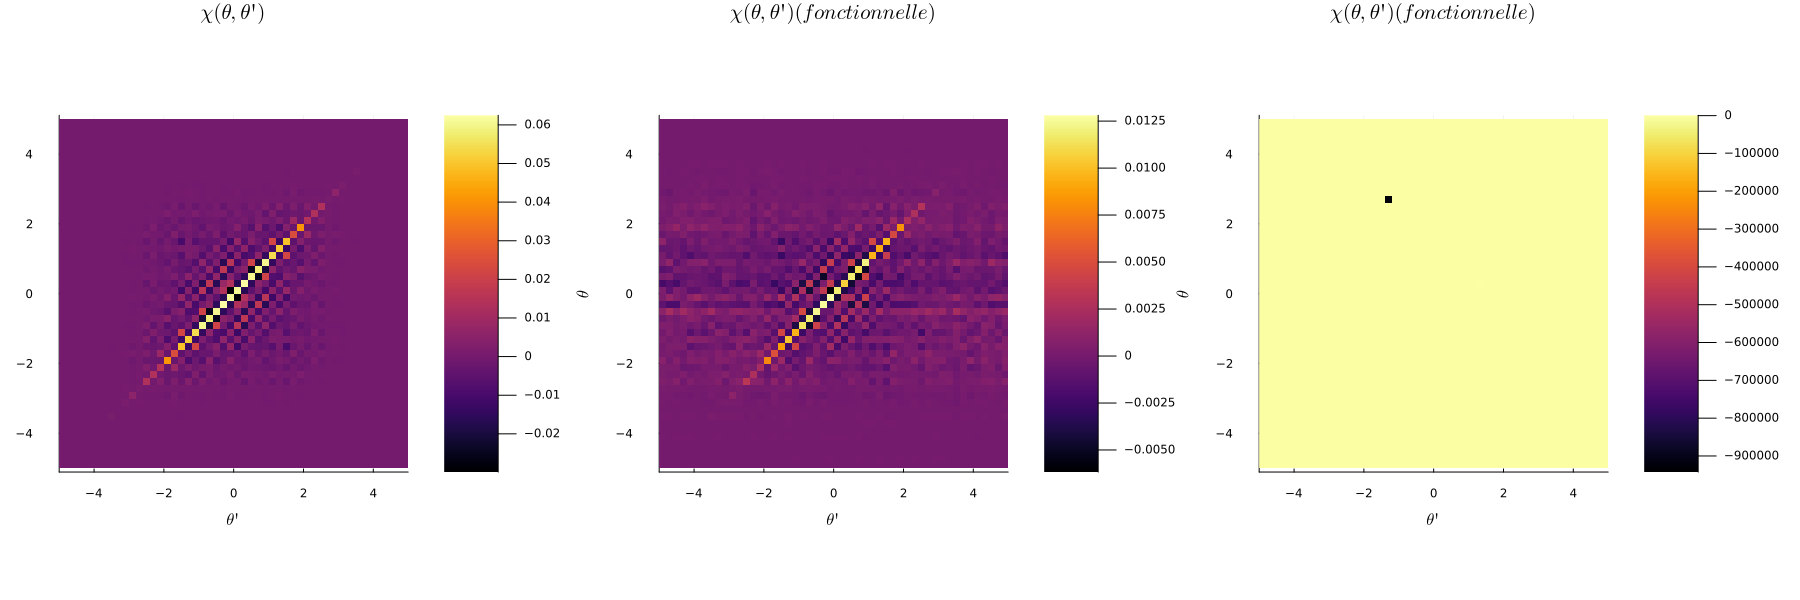
\includegraphics[width=1\textwidth]{figures/04_GGE_Fluctuation/figure_fluctuations}
    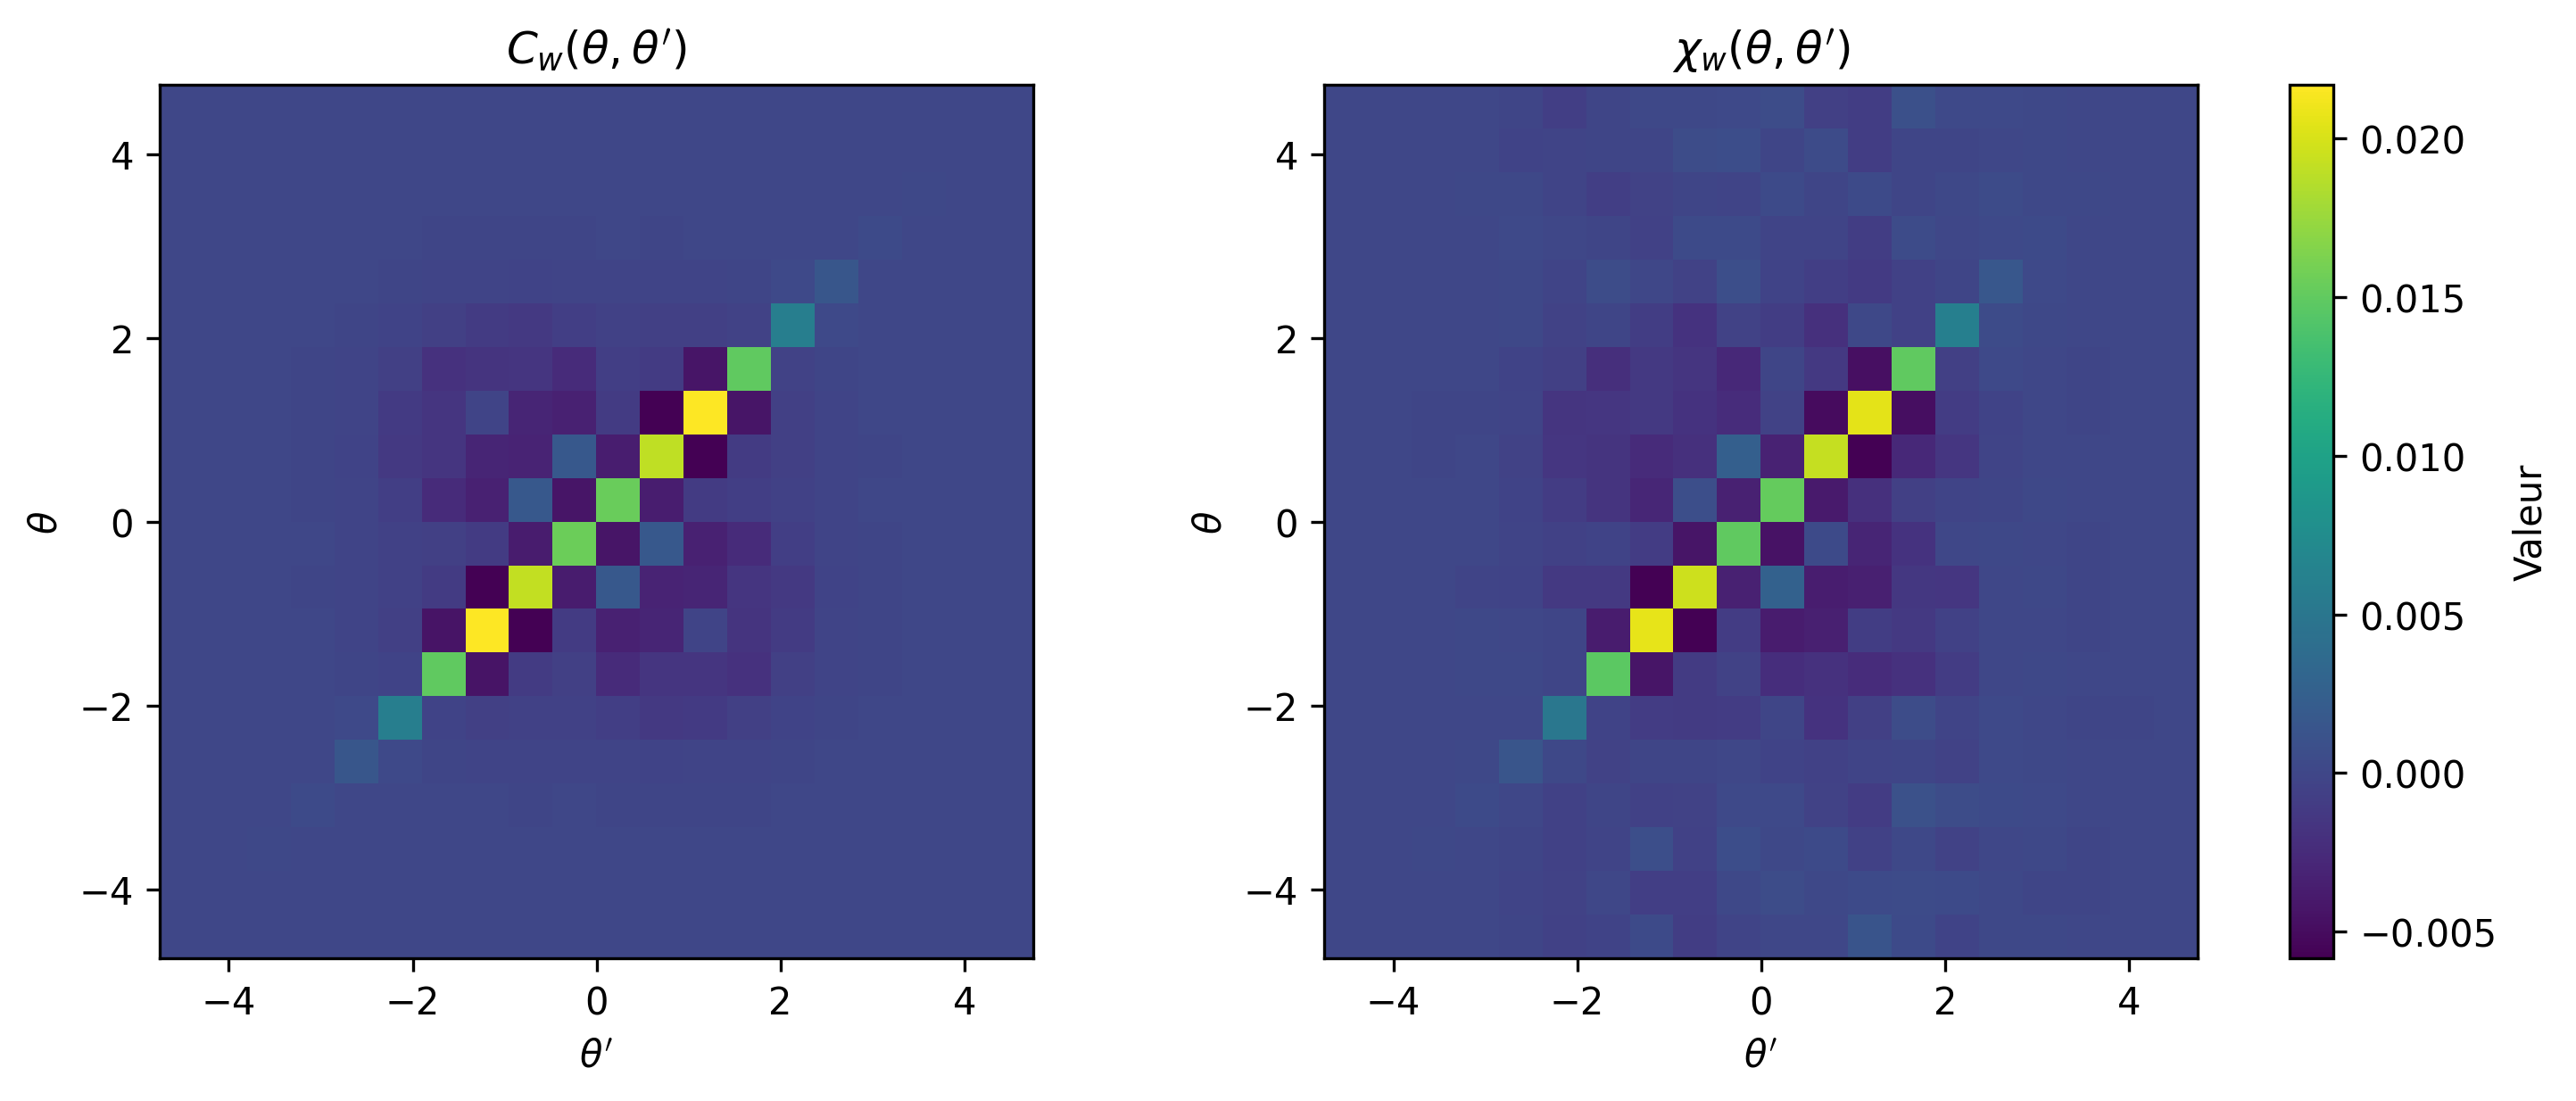
\includegraphics[width=1\textwidth]{figures/04_GGE_Fluctuation/heatmaps.png}
    \caption{Comparaison des matrices pour $\braket{\operator{\rho}(\theta)\operator{\rho}(\theta')}_w$ : à gauche la corrélation  \( C_w(\theta,\theta') \) ; à droite la susceptibilité \( \chi_w(\theta,\theta') \) obtenue par dérivée fonctionnelle pour \( N_{\rm conf} = 2 \times 10^6 \) et \( \varepsilon = 10^{-1} \).}
    \label{fig:comparison_chi_C}
\end{figure}

\paragraph{Discussion.}

Les figures montrent une concordance satisfaisante entre les deux matrices. L’écart relatif est d’environ 13,5\,\%, et provient principalement des erreurs statistiques liées à la méthode \emph{Monte Carlo} et de l’approximation par différences finies dans le calcul de la dérivée fonctionnelle.

\medskip

Le principe de fluctuation-réponse dans le cadre du \gls{GGE} étant supposé valide, l’objectif de cette analyse n’est pas de le confirmer, mais de vérifier que l’on reste en capacité d’échantillonner correctement les fluctuations à partir de \(\chi_w(\theta,\theta')\) avec un nombre fini de configurations. L’erreur relative observée est donc acceptable et reflète les limites statistiques de l’expérience numérique.

\medskip

La précision peut être améliorée en augmentant le nombre de configurations \(N_{\rm conf}\) :

% \begin{itemize}[label = $\bullet$]
% 	\item Le calcul de \(C_w(\theta, \theta')\) est en \(\mathcal{O}(N_{\rm conf})\) et celui de \(\chi_w(\theta, \theta')\) en \(\mathcal{O}(N_{\rm conf} \cdot N_{\rm cell})\), où \(N_{\rm cell}\) est le nombre de points de la grille en \(\theta\).
% 	\item Pour \(N_{\rm conf} = 2\times 10^6\) et \(N_{\rm cell} = 20\), la matrice \(C_w(\theta, \theta')\) se calcule en environ 6 minutes et \(\chi_w(\theta, \theta')\) en environ 2 heures.
% 	\item On peut envisager \(N_{\rm conf} = 10^7\) : \(C_w(\theta, \theta')\) en 30 minutes et \(\chi_w(\theta, \theta')\) en 10 heures.
% \end{itemize}

\begin{itemize}[label = $\bullet$]
    \item Dans ce point, les symboles de Landau \(\mathcal{O}(\cdot)\) désignent ici des \emph{complexités en temps de calcul}. 
    Le calcul de la matrice de corrélation \(C_w(\theta, \theta')\) s'effectue en un temps 
    de complexité \(\mathcal{O}(N_{\rm conf})\), tandis que celui de la susceptibilité 
    \(\chi_w(\theta, \theta')\) nécessite un temps de complexité 
    \(\mathcal{O}(N_{\rm conf} \cdot N_{\rm cell})\), où \(N_{\rm cell}\) est le nombre de points 
    de discrétisation de la variable \(\theta\).

    \item Pour un nombre de configurations\emph{Monte Carlo} fixé à 
    \(N_{\rm conf} = 2 \times 10^6\) et une grille de taille \(N_{\rm cell} = 20\), 
    on obtient un temps de calcul d'environ 6 minutes pour la matrice \(C_w(\theta,\theta')\), 
    tandis que le calcul de \(\chi_w(\theta,\theta')\), plus coûteux car nécessitant 
    l'évaluation d'une réponse à une perturbation sur chaque cellule, demande environ 2 heures.

    \item Si l'on augmente le nombre de configurations à 
    \(N_{\rm conf} = 10^7\), ce qui permet de réduire plus fortement le bruit statistique, 
    alors le calcul de \(C_w(\theta,\theta')\) prendrait environ 30 minutes, 
    tandis que celui de \(\chi_w(\theta,\theta')\) nécessiterait approximativement 10 heures, 
    en raison du facteur multiplicatif supplémentaire lié à la grille 
    \(\theta \mapsto \theta_i\).
\end{itemize}


\medskip

Pour de petits \(N_{\rm conf}\), la perturbation \(\varepsilon\) doit être augmentée pour que les fluctuations calculées ne soient pas noyées dans le bruit. Si \(\varepsilon\) est trop grand, on observe toujours la structure globale de \(\chi_w(\theta, \theta')\), mais avec une amplitude réduite :
\begin{eqnarray*}
	\chi_w(\theta, \theta') \approx \alpha C_w(\theta, \theta'), \quad 0 < \alpha < 1.
\end{eqnarray*}

Par exemple, pour \(N_{\rm conf} = 10^5\), la mesure \eqref{cha4:eq:std.1} est de $8\%$.  On peut utiliser \(N_{\rm cell} = 100\) et \(\varepsilon = 1\), et obtenir :
\begin{eqnarray*}
    \frac{\left\Vert  \alpha C_w - \chi_w \right\Vert_2}{\left\Vert \alpha C_w \right\Vert_2} \;\sim\; 27\%
\end{eqnarray*}
avec $\alpha = 0.078$ et pour un temps de calcul de $26~min$ (Fig~\ref{fig:comparison_chi_C_1}).
\begin{figure}[H]
    \centering
    %\includegraphics[width=0.32\textwidth]{chi_matrix.png}
    %\includegraphics[width=0.32\textwidth]{C_matrix.png}
    %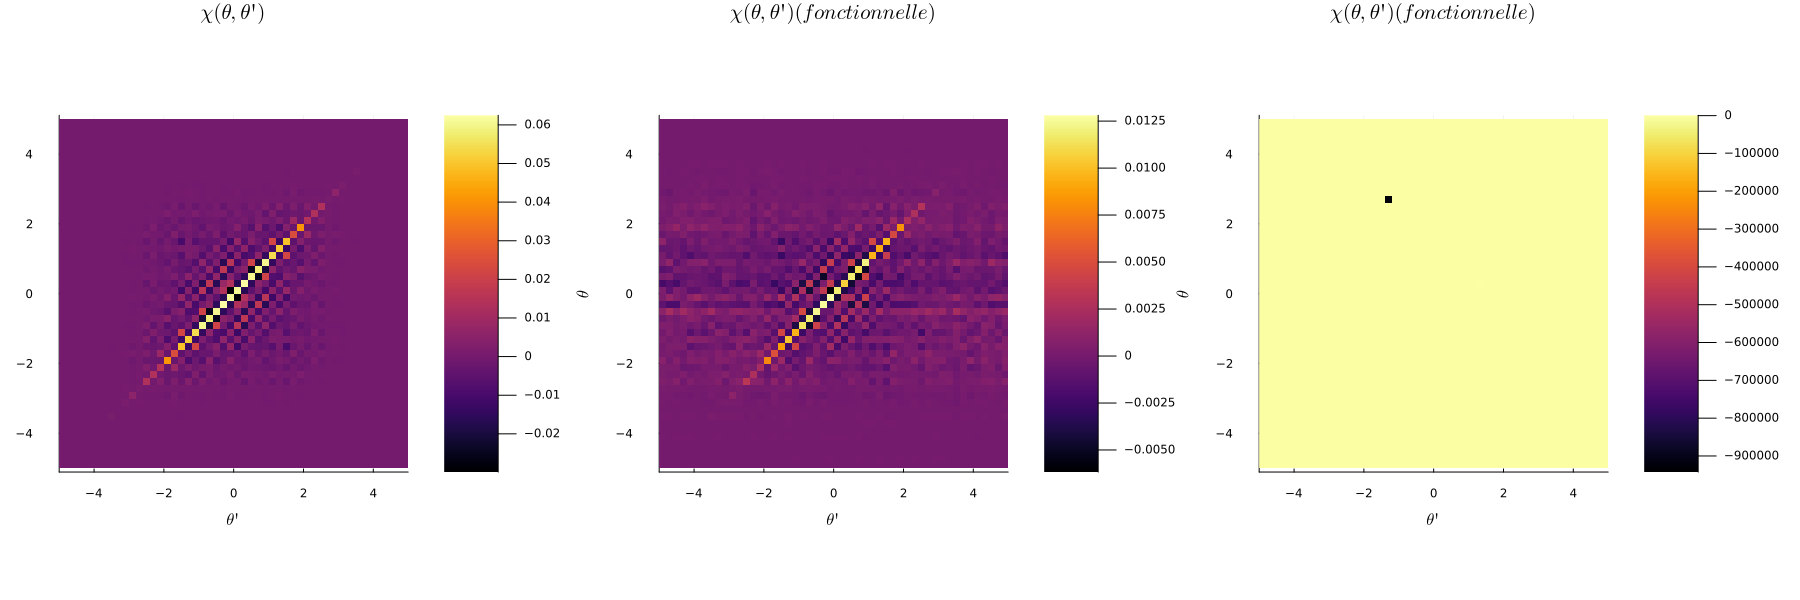
\includegraphics[width=1\textwidth]{figures/04_GGE_Fluctuation/figure_fluctuations}
    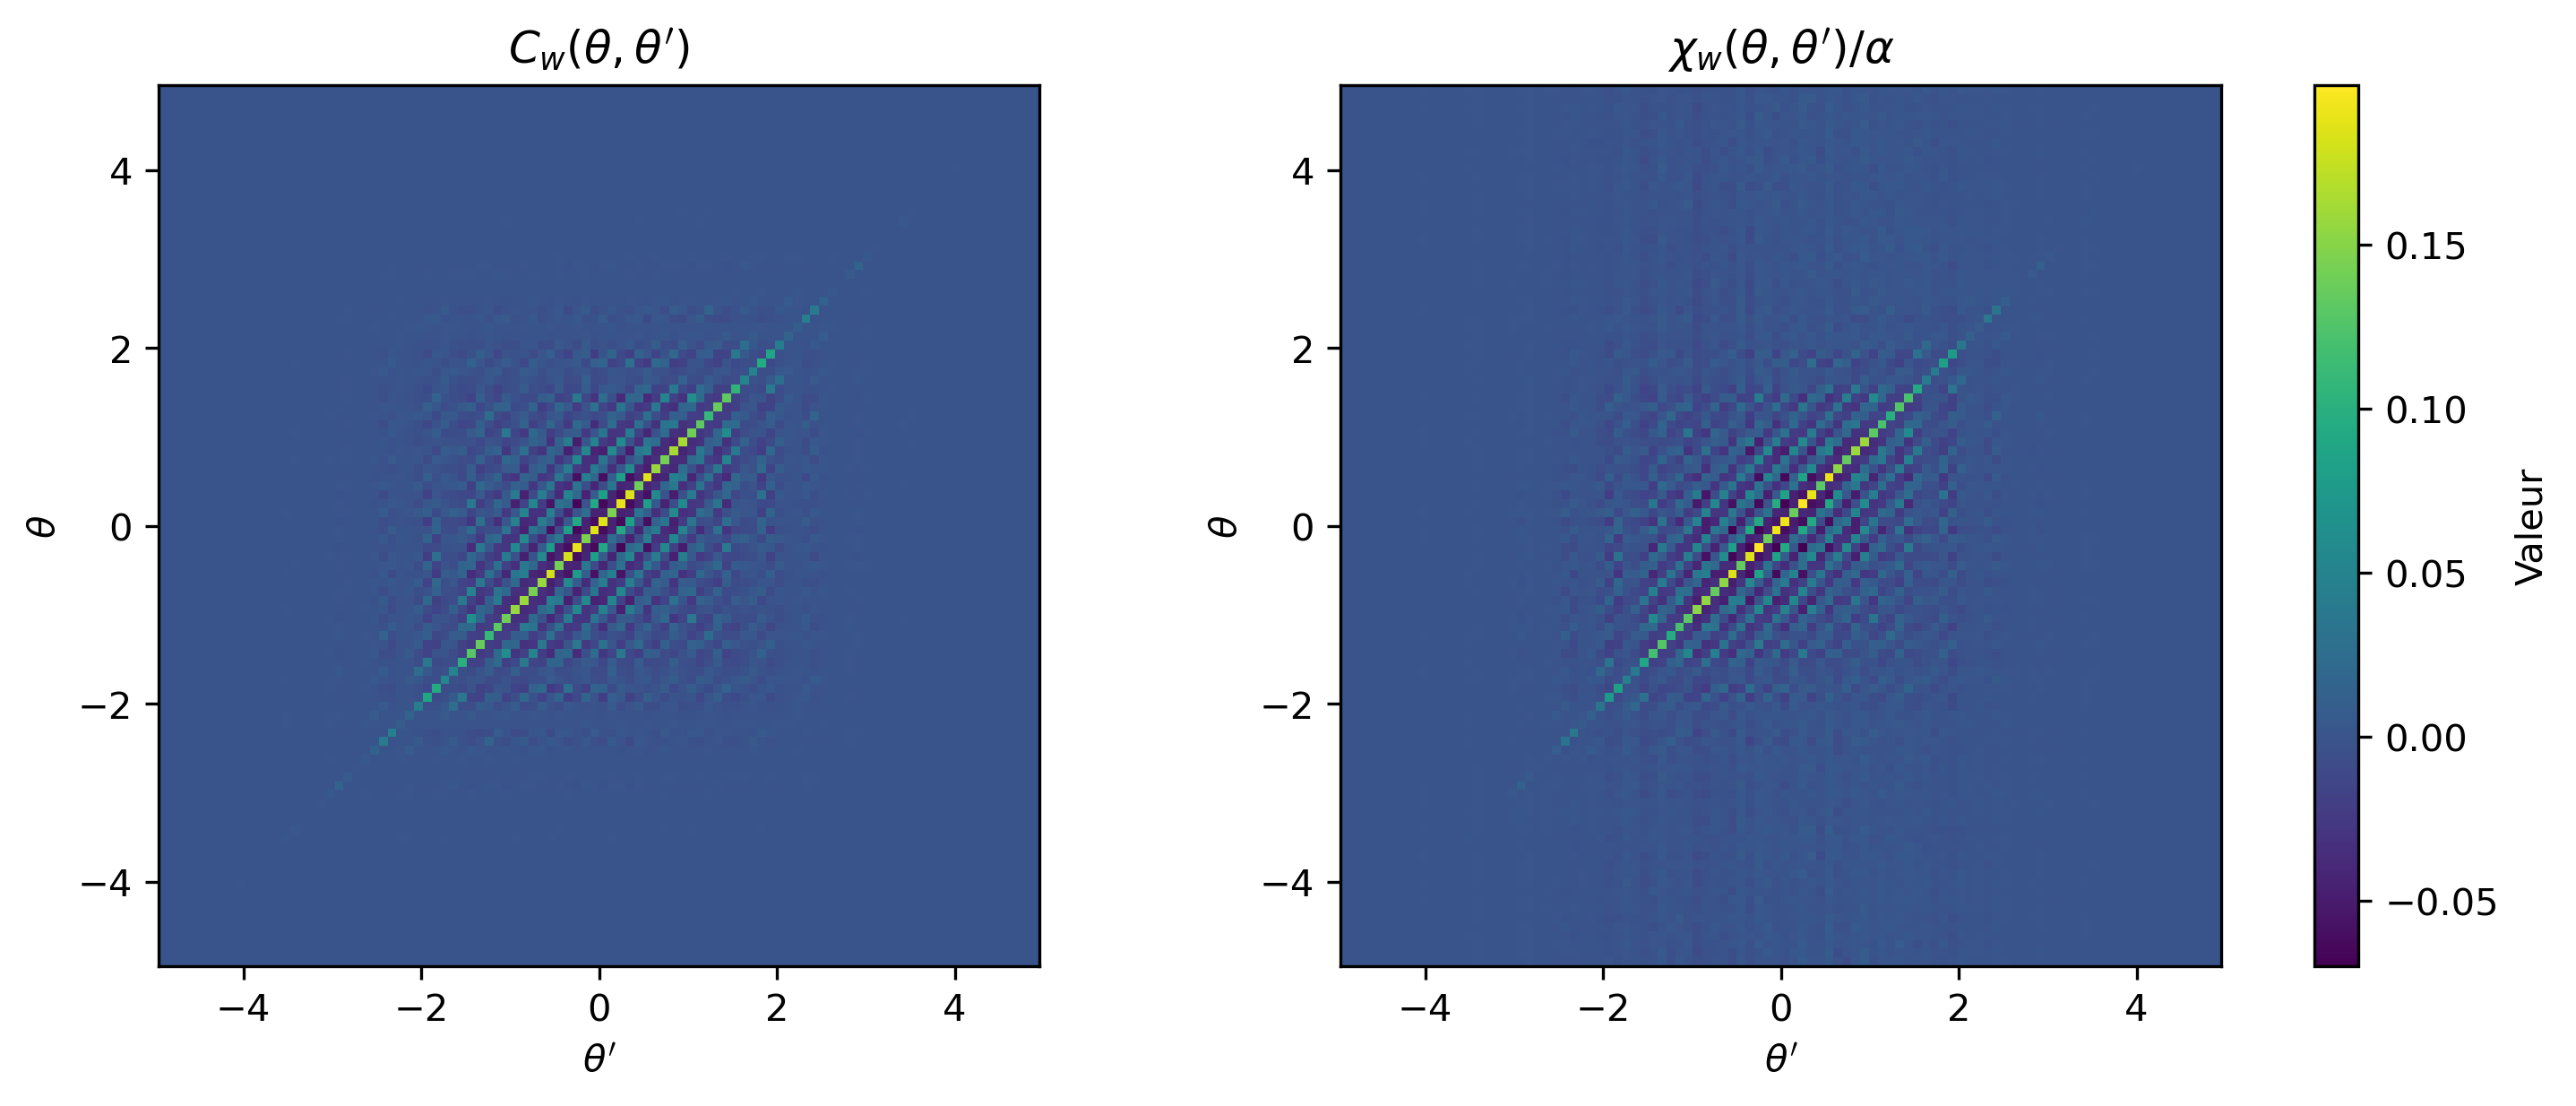
\includegraphics[width=1\textwidth]{figures/04_GGE_Fluctuation/heatmaps_1.png}
    \caption{Comparaison des matrices pour $\braket{\operator{\rho}(\theta)\operator{\rho}(\theta')}_w$ : à gauche la corrélation  \( C_w(\theta,\theta') \) ; à droite la susceptibilité \( \chi_w(\theta,\theta')/\alpha \) obtenue par dérivée fonctionnelle, pour  \(N_{\rm cell} = 100\), \(\varepsilon = 1\) et \(\alpha = 0.078\).}
    \label{fig:comparison_chi_C_1}
\end{figure}

Physiquement, \(\alpha < 1\) reflète le fait que pour un nombre limité de configurations, la réponse calculée par différences finies sous-estime légèrement l’amplitude des fluctuations par rapport à la covariance brute \(C_w\), mais la structure globale reste correcte. En augmentant \(N_{\rm conf}\), \(\alpha \to 1\) et \(\chi_w(\theta, \theta')\) converge vers \(C_w(\theta, \theta')\) dans la limite des grandes statistiques.




%On a vus dans l'equation ~\eqref{??} que pour une fonction teste quelquonque , $f \colon \mathbb{R} \to \mathbb{R}$, $\operator{\mathcal{Q}}[f]$ s'écrit de la forme integrale
%
%
%Nous avons vu que l'espérance d'une charge généralisée \( \operator{\mathcal{Q}}[f_1] \) dans cet état, notée au chapitre~(\ref{chap:relaxation}) \( \langle \operator{\mathcal{Q}}^{(\mathcal{S})}[f_1] \rangle_{\operator{\rho}_{\mathrm{GGE}}^{(\mathcal{S})}[w]} \), peut être simplifiée, dans ce chapitre, en :
%\begin{eqnarray*}
%	\langle \operator{\mathcal{Q}}[f_1] \rangle_w =  -  \left . \frac{ \delta \ln Z [w] }{ \delta f_1  } \right)_{w}  = \mathrm{Tr} \left[ \operator{\rho}_{\mathrm{GGE}}[w]\, \operator{\mathcal{Q}}[f_1] \right]
%= \frac{1}{Z[w]}\, \mathrm{Tr} \left[ e^{-\operator{\mathcal{Q}}[w]}\, \operator{\mathcal{Q}}[f_1] \right] .
%\end{eqnarray*}
%
%Par souci de lisibilité, nous omettrons les indices \((\mathcal{S})\) : le caractère local des observables étant désormais implicite.
%
%
%
%%On a vus  que l’espérance d’une observable $\operator{\mathcal{Q}}^{(\mathcal{S})}[f_1]$ dans le GGE , noté dans le chapitre \ref{} par $\langle \operator{\mathcal{Q}}^{(\mathcal{S})}[f_1] \rangle_{\operator{\rho}_{\mathrm{GGE}}^{(\mathcal{S})}[w]}$ que pour soucis d'aléger dans lé résonement on notéra $\langle \operator{\mathcal{Q}}[f_1] \rangle$, et j'enlève les $(\mathcal{S})$, le caractère locale étant maintenat inplicite , est donnée par :
%
%\medskip
%
%%La dérivée fonctionnelle de l'espérance de la charge $\operator{\mathcal{Q}}[f_1]$ par rapport au potentiel conjugué $f_2$ est donnée par :
%La dérivée fonctionnelle de l'espérance de \( \operator{\mathcal{Q}}[f_1] \) par rapport à une autre fonction test \( f_2 \), représentant un potentiel conjugué, donne la réponse linéaire croisée :
%
%\begin{eqnarray*}
%	\chi_w[f_1, f_2] \doteq   \left . \frac{ \delta^2 \ln Z [w] }{ \delta f_1 \delta f_2 } \right)_{w} =  - \left.\frac{\delta \langle \operator{\mathcal{Q}}[f_1] \rangle}{\delta f_2} \right )_w = C_w[f_1, f_2] ,
%\end{eqnarray*}
%
%avec le fonction corrélation à deux points :
%
%\begin{eqnarray*}
%	C_w[f_1, f_2] \doteq  	\langle ( \operator{\mathcal{Q}}[f_1] - \langle \operator{\mathcal{Q}}[f_1] \rangle_w ) ( \operator{\mathcal{Q}}[f_2] - \langle \operator{\mathcal{Q}}[f_f] \rangle_w  ) \rangle_w = \langle \operator{\mathcal{Q}}[f_1] \operator{\mathcal{Q}}[f_2] \rangle_w - \langle \operator{\mathcal{Q}}[f_1] \rangle_w \langle \operator{\mathcal{Q}}[f_2] \rangle_w.
%\end{eqnarray*}
%
%
%Autrement dit, la dérivée fonctionnelle seconde du logarithme de la fonction de partition fournit la covariance des charges \( \operator{\mathcal{Q}}[f_1] \) et \( \operator{\mathcal{Q}}[f_2] \), illustrant le principe de fluctuation-réponse dans ce contexte diagonal.
%
%\paragraph{Démonstration.}
%
%Pour établir le lien entre réponse linéaire et fluctuations, nous allons partir de l'expression intégrale des charges généralisées, puis montrer que la susceptibilité associée correspond bien à la fonction de corrélation des fluctuations de densité de rapidité.
%
%
%\subparagraph{Charge généralisé sous forme intégrale.}
%Pour le démontrer on écrit la charge généralisé sous forme intégrale :
%\begin{eqnarray*}
%\operator{\mathcal{Q}}[f] = L\int d\theta f(\theta) \operator{\rho}(\theta)
%\end{eqnarray*}
%où $\operator{\rho}(\theta)$ est l'opérateur densité spectal , agissant comme :
%\(
%\operator{\rho}(\theta) \ket{ \{ \theta_a \} } = \frac{1}{L} \sum \delta ( \theta - \theta_a ) \ket{ \{ \theta_a \} }.
%\)
%
%\subparagraph{Dérivée fonctionnelle.}
%On dérive cette expression par rapport à $w_2$. En utilisant la dérivée d’un rapport :
%\(
%	\left.\frac{\delta}{\delta f_2} \left( \frac{A[w]}{Z[w]} \right) \right |_{w} = \frac{1}{Z[w]}\, \left.\frac{\delta A[w]}{\delta f_2} \right|_{w} - \frac{A[w]}{Z[w]^2}\, \left.\frac{\delta Z[w]}{\delta f_2}\right|_{w} ,
%\)
%avec $A[w] \equiv \mathrm{Tr}[e^{-\operator{\mathcal{Q}}[w]} \operator{\mathcal{Q}}[f_1]]$, on obtient :
%\begin{eqnarray*}
%	\left . \frac{\delta \langle \operator{\mathcal{Q}}[f_1] \rangle_w}{\delta f_2} \right )_w
%	= \frac{1}{Z[w]}\, \frac{\delta A[w]}{\delta f_2}
%	- \langle \operator{\mathcal{Q}}[f_1] \rangle_w \cdot \frac{1}{Z[w]}\, \frac{\delta Z[w]}{\delta f_2}.
%\end{eqnarray*}
%
%\subparagraph{Dérivées explicites.}
%Utilisons la propriété démontrée précédemment :
%\(
%	\frac{\delta \operator{\mathcal{Q}}[w]}{\delta f_2} = \operator{\mathcal{Q}}[f_2]	.
%\)
%En notant que la dérivée d’une exponentielle diagonale est simple :
%\(
%\frac{\delta}{\delta f_2} e^{-\operator{\mathcal{Q}}[w]} = - \operator{\mathcal{Q}}[f_2]\, e^{-\operator{\mathcal{Q}}[w]},
%\)
%on obtient :
%\begin{eqnarray*}
%\frac{\delta A[w]}{\delta f_2} = - \mathrm{Tr}\left[ \operator{\mathcal{Q}}[f_2]\, e^{-\operator{\mathcal{Q}}[w]} \operator{\mathcal{Q}}[f_1] \right],
%\quad
%\frac{\delta Z[w]}{\delta f_2} = - \mathrm{Tr}\left[ \operator{\mathcal{Q}}[f_2]\, e^{-\operator{\mathcal{Q}}[w]} \right].
%\end{eqnarray*}
%
%\subparagraph{Regroupement.}
%En regroupant les termes, on trouve :
%\begin{eqnarray*}
%	\chi_w[f_1, f_2]&  \doteq & - \left.\frac{\delta \langle \operator{\mathcal{Q}}[f_1] \rangle_w}{\delta f_2} \right )_w  \\
%&=& \frac{1}{Z[w]}\, \mathrm{Tr}\left[ \operator{\mathcal{Q}}[w_2]\, e^{-\operator{\mathcal{Q}}[w]}\, \operator{\mathcal{Q}}[f_1] \right]
%- \langle \operator{\mathcal{Q}}[f_1] \rangle_w \cdot \frac{1}{Z[w]}\, \mathrm{Tr}\left[ \operator{\mathcal{Q}}[f_2]\, e^{-\operator{\mathcal{Q}}[w]} \right] \\
%&=& \langle \operator{\mathcal{Q}}[f_2]\, \operator{\mathcal{Q}}[f_1] \rangle_w - \langle \operator{\mathcal{Q}}[f_1] \rangle_w\, \langle \operator{\mathcal{Q}}[f_2] \rangle_w.
%\end{eqnarray*}
%
%\medskip
%
%\subparagraph{Conclusion.} Dans un état diagonal tel que le GGE, la susceptibilité est égale à la covariance entre charges généralisées, illustrant le principe de \emph{fluctuation-réponse}.
%%\paragraph{Remarques.}
%La matrice $\chi_w[f_1, f_2]$ s’interprète donc comme la covariance de la densité spectrale projetée sur les fonctions test $f_1$ et $f_2$.
%Un cas particulier d’intérêt est la susceptibilité d’une seule charge :
%\begin{eqnarray*}
%\chi_w[f] \equiv \chi_w[f, f] = \mathrm{Var}_w(\operator{\mathcal{Q}}[f]) = \langle \operator{\mathcal{Q}}[f]^2 \rangle_w - \langle \operator{\mathcal{Q}}[f] \rangle_w^2
%= L^2 \iint d\theta\, d\theta'\, f(\theta)\, C_w(\theta, \theta')\, f(\theta').
%\end{eqnarray*}
%
%
%\subsection{Corrélations spectrales et susceptibilité}
%
%%\paragraph{Corrélations spectrales et susceptibilité.}
%
%La susceptibilité fonctionnelle peut s’exprimer, dans la base des fonctions test, comme une forme bilinéaire projetée sur la fonction de corrélation spectrale :
%\begin{eqnarray*}
%\chi_w[f_1, f_2] = C_w[f_1, f_2] = L^2 \iint d\theta\, d\theta'\, f_1(\theta)\, C_w(\theta, \theta')\, f_2(\theta'),
%\end{eqnarray*}
%où la fonction de corrélation spectrale \( C_w(\theta, \theta') \) est définie comme la covariance des fluctuations de densité spectrale :
%\begin{eqnarray*}
%C_w(\theta, \theta') \doteq \langle \delta \operator{\rho}(\theta)\, \delta \operator{\rho}(\theta') \rangle_w = \langle \operator{\rho}(\theta)\, \operator{\rho}(\theta') \rangle_w - \langle \operator{\rho}(\theta) \rangle_w\, \langle \operator{\rho}(\theta') \rangle_w.
%\end{eqnarray*}
%
%Par ailleurs, l’espérance de la densité spectrale s’obtient comme une dérivée fonctionnelle du logarithme de la fonction de partition :
%\begin{eqnarray*}
%\langle \operator{\rho}(\theta) \rangle_w = - \frac{1}{L} \left. \frac{\delta \ln Z[w]}{\delta w(\theta)} \right),
%\end{eqnarray*}
%et la susceptibilité spectrale, définie comme la réponse de \( \langle \rho(\theta) \rangle_w \) à une variation de \( w(\theta') \), s’écrit :
%\begin{eqnarray*}
%\chi_w(\theta, \theta') = \left. \frac{1}{L^2} \frac{\delta^2 \ln Z[w]}{\delta w(\theta)\, \delta w(\theta')} \right) = - \left. \frac{1}{L} \frac{\delta \langle \operator{\rho}(\theta) \rangle_w}{\delta w(\theta')} \right).
%\end{eqnarray*}
%
%Ainsi, dans l’état diagonal \( \operator{\rho}_{\mathrm{GGE}}[w] \), la susceptibilité spectrale coïncide avec la fonction de corrélation \( C_w(\theta, \theta') \), illustrant le principe de \emph{fluctuation-réponse}.
%



\section{Limite thermodynamique, structure variationnelle et susceptibilité}

\subsection{Susceptibilité spectrale et structure variationnelle de l’entropie}

\begin{mdframed}[
	linewidth=0.5pt,
	backgroundcolor=gray!5,
	roundcorner=50pt,
	innerleftmargin=5pt,
    innerrightmargin=5pt,
    innertopmargin=-10pt,
    innerbottommargin=2pt,
    leftmargin=2pt,
    rightmargin=2pt
	]
\paragraph{Rappel : Approche thermodynamique (Yang–Yang et énergie généralisée).}

Dans l’approximation thermodynamique, le sous-système est décrit en termes de grandeurs macroscopiques, notamment par la distribution de rapidité $\rho(\theta)$.
Dans l’équation \eqref{chap:TBA:eq:ensemble_average}, nous avons vu que, dans la limite thermodynamique, la moyenne d’une observable s’écrit :
\begin{eqnarray}
	\langle \operator{\mathcal{O}} \rangle_{w} & = & \frac{\int \mathcal{D} \rho \; e^{L (\mathcal{S}_{YY}[\rho] - \mathcal{W}[\rho])} \, \langle\operator{\mathcal{O}}\rangle_{[\rho]}}{\int \mathcal{D} \rho \; e^{L (\mathcal{S}_{\mathrm{YY}}[\rho] - \mathcal{W}[\rho])}}. \label{chap:Fluc:eq:ensemble_average}
\end{eqnarray}
où $\mathcal{S}_{\mathrm{YY}}$ est l’entropie de \gls{YY} et $\mathcal{W}$ l’énergie généralisée, introduites respectivement dans \eqref{chap.2.entropi.int} et \eqref{chap.2.W.int}, que l'on rappelle.
\begin{eqnarray}
	\mathcal{S}_{YY}[\rho] & = & \int d \theta  \, [ \rho_s\ln \rho_s - \rho \ln \rho - ( \rho_s - \rho ) \ln ( \rho_s - \rho ) ] (\theta) , \label{chap.4.entropi.int}\\
	\mathcal{W}[\rho] & = & \int   w(\theta) \rho(\theta) \, d \theta, \label{chap.4.W.int}
\end{eqnarray}
où \(\rho_s(\theta)\) désigne la {\em densité d’états} liée à \(\rho\) par les équations de \gls{BA} \eqref{eq:TBA-rhos} :
\begin{eqnarray}
	2\pi \rho_s = 1 + \Delta \star \rho.
\end{eqnarray}

\medskip

La quantité $\langle\operator{\mathcal{O}}\rangle_{[\rho]}$ désigne la valeur propre de l’observable associée aux états caractérisés par la distribution de rapidité $\rho$.




\end{mdframed}

\medskip

\begin{mdframed}[
	linewidth=0.5pt,
	backgroundcolor=gray!5,
	roundcorner=50pt,
	innerleftmargin=5pt,
    innerrightmargin=5pt,
    innertopmargin=-10pt,
    innerbottommargin=2pt,
    leftmargin=2pt,
    rightmargin=2pt
]
\paragraph{Rappel : Condition variationnelle du GGE.}


À l’équilibre thermodynamique; dans la limite $L \to \infty$, la distribution $\rho_{\mathrm{eq}}(\theta)$ satisfait l’équation \eqref{chap.2:eq.rho.eq.1}, et coïncide alors avec la moyenne de l’opérateur de densité de rapidité :
\begin{eqnarray}
	 \rho_{\mathrm{eq}}(\theta) =  \braket{ \operator{\rho}(\theta) }_w,
\end{eqnarray}
représentant ainsi la densité continue de quasi-particules dans l’état stationnaire / d’équilibre.


\medskip

Dans le cadre du \gls{GGE} continu, l’état macroscopique est entièrement déterminé par la densité spectrale $\rho(\theta)$ qui maximise l’entropie de \acrlong{YY}, $\mathcal{S}_{\mathrm{YY}}[\rho]$, sous la contrainte de conservation des charges généralisées. Le poids spectral $w(\theta)$ est alors fixé.
Comme nous l’avons vu (au chapitre~(\ref{chap:relaxation})), la condition d’équilibre \eqref{chap:TBA:eq:stationnarite-3} peut s’écrire sous la forme variationnelle :
\begin{eqnarray}
	\left. \frac{\delta \mathcal{S}_{\mathrm{YY}}[\rho]}{\delta \rho(\theta)} \right)_{\rho = \rho_{\mathrm{eq}}} = w(\theta). \label{chap:Fluc:eq:stationnarite-3}
\end{eqnarray}

\end{mdframed}

%\begin{mdframed}[
%	linewidth=0.5pt,
%	backgroundcolor=gray!5,
%	roundcorner=50pt,
%	innerleftmargin=5pt,
%    innerrightmargin=5pt,
%    innertopmargin=-10pt,
%    innerbottommargin=2pt,
%    leftmargin=2pt,
%    rightmargin=2pt
%]
%\paragraph{Rappel : Approche thermodynamique (\gls{YY} et énergie généralisée).}
%
%Dans l’approximation thermodynamique, le système est décrit en termes de grandeurs macroscopiques, notamment par la distribution de rapidité $\rho(\theta)$.
%Dans l’équation \eqref{chap:TBA:eq:ensemble_average}, la moyenne d’un observable s’écrit, dans la limite thermodynamique :
%\begin{eqnarray}
%	\langle \operator{\mathcal{O}} \rangle_{w} & = &
%	\frac{\int \mathcal{D} \rho \; e^{L (\mathcal{S}_{YY}[\rho] - \mathcal{W}[\rho])} \,
%	\langle\operator{\mathcal{O}}\rangle_{[\rho]}}
%	{\int \mathcal{D} \rho \; e^{L (\mathcal{S}_{\mathrm{YY}}[\rho] - \mathcal{W}[\rho])}}.
%	\label{chap:Fluc:eq:ensemble_average}
%\end{eqnarray}
%où $\mathcal{S}_{\mathrm{YY}}$ est l’entropie de \gls{YY} et $\mathcal{W}$ l’énergie généralisée :
%\begin{eqnarray}
%	\mathcal{S}_{YY}[\rho] & = & \int d \theta
%	\big[ \rho_s\ln \rho_s - \rho \ln \rho - ( \rho_s - \rho ) \ln ( \rho_s - \rho ) \big] (\theta),
%	\label{chap.4.entropi.int}\\
%	\mathcal{W}[\rho] & = & \int   w(\theta) \rho(\theta) \, d \theta,
%	\label{chap.4.W.int}
%\end{eqnarray}
%avec $\rho_s(\theta)$ la densité d’états reliée à $\rho$ par les équations de \gls{BA} \eqref{eq:TBA-rhos} :
%\begin{eqnarray}
%	2\pi \rho_s = 1 + \Delta \star \rho.
%\end{eqnarray}
%\end{mdframed}
%
%\begin{mdframed}[
%	linewidth=0.5pt,
%	backgroundcolor=gray!5,
%	roundcorner=50pt,
%	innerleftmargin=5pt,
%    innerrightmargin=5pt,
%    innertopmargin=-10pt,
%    innerbottommargin=2pt,
%    leftmargin=2pt,
%    rightmargin=2pt
%]
%\paragraph{Rappel : Condition variationnelle du GGE.}
%
%À l’équilibre thermodynamique, la distribution $\rho_{\mathrm{eq}}(\theta)$ coïncide avec la moyenne de l’opérateur de densité de rapidité :
%\begin{eqnarray}
%	 \rho_{\mathrm{eq}} =  \braket{ \operator{\rho}(\theta) }_w.
%\end{eqnarray}
%
%Dans le cadre du GGE continu, l’état macroscopique est entièrement déterminé par une densité spectrale $\rho(\theta)$ qui maximise l’entropie de \gls{YY}, $\mathcal{S}_{\mathrm{YY}}[\rho]$, sous contrainte des charges généralisées. Le poids spectral $w(\theta)$ est alors fixé.
%
%La condition d’équilibre peut s’écrire sous forme variationnelle :
%\begin{eqnarray}
%	\left. \frac{\delta \mathcal{S}_{\mathrm{YY}}[\rho]}{\delta \rho(\theta)} \right|_{\rho = \rho_{\mathrm{eq}}}
%	= w(\theta).
%	\label{chap:Fluc:eq:stationnarite-3}
%\end{eqnarray}
%\end{mdframed}
%


\medskip
\paragraph{Dérivée fonctionnelle.}
On peut considérer l’équation d’équilibre comme une relation implicite définissant le poids spectral $w$ comme une fonctionnelle de la distribution de rapidité $\rho$. La dérivée fonctionnelle de cette relation s’écrit :
\begin{eqnarray}
	\left. \frac{\delta w(\theta)}{\delta \rho(\theta')} \right)_{\rho = \rho_{\mathrm{eq}}} = \left. \frac{\delta^2 \mathcal{S}_{\mathrm{YY}}[\rho]}{\delta \rho(\theta)\, \delta \rho(\theta')} \right)_{\rho = \rho_{\mathrm{eq}}}, \label{chap:Fluc:eq:susp-1}
\end{eqnarray}
où le membre de droite représente l’opérateur hessien (ou courbure fonctionnelle) de l'entropie de \gls{YY}, évalué à l’équilibre. Cet opérateur est défini négatif, conformément à l’interprétation de $\mathcal{S}_{\mathrm{YY}}$ comme une entropie à maximiser.

\paragraph{Inversion.}
On en déduit que la réponse de $\rho$ à une variation infinitésimale du poids spectral $w$ est donnée par l'inverse fonctionnel de \eqref{chap:Fluc:eq:susp-1} :
\begin{eqnarray}
	-\frac{1}{L} \left. \frac{\delta \rho(\theta)}{\delta w(\theta')} \right)_{\rho = \rho_{\mathrm{eq}}} = - \left( L \left. \frac{\delta^2 \mathcal{S}_{\mathrm{YY}}[\rho]}{\delta \rho(\theta)\, \delta \rho(\theta')} \right)_{\rho = \rho_{\mathrm{eq}}} \right)^{-1}. \label{chap:Fluc:eq:susp-2}
\end{eqnarray}
La susceptibilité fonctionnelle $\chi_w(\theta, \theta')$, définie dans \eqref{chap4:eq.susceptibilite-fonctionnelle_3}, coïncide avec cette expression.


\subsection{Fluctuations gaussiennes autour de l’équilibre thermodynamique}

Une autre approche pour accéder aux fluctuations de la distribution de rapidité $\rho = \rho_{\mathrm{eq}} + \delta \rho $  est d'étudier la structure variationnelle de l’action effective $\mathcal{S}_{YY} - \mathcal{W}$ autour du point d’équilibre $\rho_{\mathrm{eq}}$. En effet, par définition de ce point d’équilibre, toute variation infinitésimale $\delta \rho$ satisfait  \cite{Wheeler_FieldTheory_Ch5}:
\begin{eqnarray*}
	(\mathcal{S}_{YY} - \mathcal{W})[\rho_{\mathrm{eq}} + \delta \rho ]  = \exp \{\dfonc{\delta \rho }\}\left ( (\mathcal{S}_{YY} - \mathcal{W})[\rho_{\mathrm{eq}}] \right ).
\end{eqnarray*}
%Dans un état de \gls{GGE} consiste à exploiter le développement quadratique de l’action effective autour de l’équilibre thermodynamique. Cette méthode, dite \emph{gaussienne}, repose sur le fait que, dans la limite thermodynamique, l’intégrale fonctionnelle définissant le GGE est dominée par les configurations proches du point-selle $\rho_{\mathrm{eq}}$.
Dans la limite thermodynamique, l’intégrale fonctionnelle définissant le \gls{GGE} est dominée par les configurations proches de l'extremum $\rho_{\mathrm{eq}}$. Cette approximation, dite gaussienne, repose alors sur le développement quadratique de la {\em fonction thermodynamique effective} $\mathcal{S}_{YY} - \mathcal{W}$ en $\delta \rho$.

\smallskip

On peut ainsi développer la {\em fonction thermodynamique effective} $\mathcal{S}_{YY} - \mathcal{W}$  au second ordre autour de ce point d'équilibre :
%\begin{eqnarray}
%	(\mathcal{S}_{YY} - \mathcal{W})[\rho] \approx (\mathcal{S}_{YY} - \mathcal{W})[\rho_{\mathrm{eq}}]  + \underbrace{\int d\theta \left . \frac{ \delta (\mathcal{S}_{YY} - \mathcal{W})[\rho]}{\delta \rho (\theta) }  \right)_{\rho = \rho_{eq} } \delta \rho(\theta)}_{\text{= 0 par stationnarité}} - \frac{1}{2} \int d\theta d \theta' \delta \rho(\theta) \mathcal{H}(\theta, \theta' )\delta \rho(\theta') + \mathcal{O}(\delta \rho^3)
%\end{eqnarray}
\begin{eqnarray}
	(\mathcal{S}_{YY} - \mathcal{W})[\rho] \approx (\mathcal{S}_{YY} - \mathcal{W})[\rho_{\mathrm{eq}}]   - \frac{1}{2} \int d\theta d \theta' \delta \rho(\theta) \mathcal{H}(\theta, \theta' )\delta \rho(\theta') + \mathcal{O}(\delta \rho^3)
\end{eqnarray}
où
\(
\displaystyle \mathcal{H}(\theta, \theta' ) = -\left.\frac{\delta^{2}(\mathcal{S}_{YY}-\mathcal{W})[\rho]}{\delta\rho(\theta)\,\delta\rho(\theta')}\right)_{\rho = \rho_{\mathrm{eq}}}
\)
est la \emph{matrice hessienne} de la {\em fonction thermodynamique effective}.

\smallskip

Sous l’approximation gaussienne autour de l’état d’équilibre (en particulier lorsque \(L \to \infty\), cf. Fig.~\ref{fig:Act.gauss}), la covariance des fluctuations s’exprime comme suit :
\begin{eqnarray}
\langle \delta \rho(\theta) \, \delta \rho(\theta') \rangle_w &=& \frac{
 \displaystyle \int \mathcal{D} \delta \rho \; \delta \rho(\theta) \, \delta \rho(\theta')
    \, \exp \left[
        -\frac{L}{2}
        \iint  d \theta_1 d \theta_2 \;
        \delta \rho(\theta_1) \, \mathcal{H}(\theta_1, \theta_2 )  \, \delta \rho(\theta_2)
    \right]
}{
    \displaystyle \int \mathcal{D} \delta \rho \;
    \exp \left[
        -\frac{L}{2}
        \iint  d \theta_1 d \theta_2 \;
        \delta \rho(\theta_1) \, \mathcal{H}(\theta_1, \theta_2 )  \, \delta \rho(\theta_2)
    \right]
}, \nonumber \\
&=& (L \mathcal{H})^{-1}(\theta, \theta' ), \label{eq:fluctuations}
\label{chap:fluctu:eq:fluctuations}.
\end{eqnarray}
%Les corrélation $C_w(\theta, \theta')$ définie en \eqref{chap4:eq.corre.2} coïncide avec cette expression .

\medskip

Ces relations posent les bases d'une description quantifiée des fluctuations de densité de rapidité, essentielles pour tester expérimentalement la validité du \gls{GGE}, particulièrement pour la mesure des  corrélations à longue distance, et accéder aux propriétés dynamiques fines des systèmes intégrables en une dimension.

\smallskip

Ce développement quadratique justifie le caractère gaussien des fluctuations dans le régime thermodynamique, et sera à la base des extensions hydrodynamiques de type \gls{MFT}.

\paragraph{Structure de \(\mathcal{H}\).}

L’opérateur hessien de l’action effective se décompose naturellement comme la différence entre deux contributions fonctionnelles :
\begin{eqnarray}
	\mathcal{H} = \mathcal{H}^{(\mathcal{W})} - \mathcal{H}^{(\mathcal{S}_{\mathrm{YY}})},
\end{eqnarray}
\begin{eqnarray}
	\mbox{où} \quad \mathcal{H}^{(\mathcal{W})}(\theta,\theta') \doteq \left. \frac{\delta^2 \mathcal{W}[\rho]}{\delta \rho(\theta)\, \delta \rho(\theta')} \right)_{\rho = \rho_{\mathrm{eq}}}, \quad \text{et} \quad \mathcal{H}^{(\mathcal{S}_{\mathrm{YY}})}(\theta,\theta') \doteq \left. \frac{\delta^2 \mathcal{S}_{\mathrm{YY}}[\rho]}{\delta \rho(\theta)\, \delta \rho(\theta')} \right)_{\rho = \rho_{\mathrm{eq}}}.
\end{eqnarray}

\medskip


L’opérateur inverse \(\mathcal{H}^{-1}\) est défini par la relation fonctionnelle :
\begin{eqnarray}
	(\mathcal{H}^{-1} \cdot \mathcal{H})(\theta, \theta') = (\mathcal{H} \cdot \mathcal{H}^{-1})(\theta, \theta') = \int d\theta'' \; \mathcal{H}(\theta, \theta'')\, \mathcal{H}^{-1}(\theta'', \theta') = \delta(\theta - \theta'),
	\label{chap:fluctu:eq:hessienner.prod.inv}
\end{eqnarray}
où \(\delta(\theta - \theta')\) désigne la distribution de Dirac, et non une variation.

\medskip

On remarque tout d’abord que \(\mathcal{H}^{(\mathcal{W})} = 0\), car l’énergie généralisée par unité de longueur s’écrit simplement comme un couplage linéaire en \(\rho\)
%\begin{eqnarray*}
%	\mathcal{W}[\rho] = \int d\theta \, w(\theta)\, \rho(\theta),
%\end{eqnarray*}
avec un poids spectral \(w(\theta)\) fixé \eqref{chap.4.W.int}.% La seconde dérivée fonctionnelle de \(\mathcal{W}\) s’annule donc identiquement.

\medskip

La courbure fonctionnelle provient donc entièrement de l'entropie de \gls{YY}, donnée par l’expression \eqref{chap.4.entropi.int}.
%\begin{eqnarray}
%	\mathcal{S}_{\mathrm{YY}}[\rho] = \int d\theta \left[
%	\rho_s(\theta) \ln \rho_s(\theta) - \rho(\theta) \ln \rho(\theta) - (\rho_s(\theta) - \rho(\theta)) \ln(\rho_s(\theta) - \rho(\theta))
%	\right] \label{chap.4.entropi.int},
%\end{eqnarray}

\medskip

Ainsi, l’opérateur de fluctuation \(\mathcal{H}\) coïncide avec la hessienne négative de l'entropie \(\mathcal{S}_{\mathrm{YY}}\), et détermine complètement la covariance spectrale à l’équilibre.


%\paragraph{Interprétation.}
%La matrice $\chi(\theta, \theta')$ possède plusieurs interprétations équivalentes :
%\begin{itemize}[label = $\bullet$]
%  \item Elle mesure la réponse linéaire de la densité spectrale à une variation du potentiel conjugué :
%  \[
%  \chi_w(\theta, \theta') = - \frac{1}{L}\frac{\delta \rho_{\mathrm{eq}}(\theta)}{\delta w(\theta')}.
%  \]
%  \item Dans un état diagonal (comme le GGE), elle coïncide avec la matrice de corrélation, selon le principe fluctuation-réponse :
%  \[
%  \chi_w(\theta, \theta') = \langle \delta \operator{\rho}(\theta)\, \delta \operator{\rho}(\theta') \rangle_w%- \frac{1}{L}\frac{\delta \langle  \operator{\rho}(\theta) \rangle_w}{\delta w(\theta')}.
%  \]
%  \item Dans la limite thermodynamique, où $\operator{\rho}(\theta) \to \rho(\theta)$, on peut omettre les chapeaux :
%  \[
%  \chi_w(\theta, \theta') = \langle \delta \rho(\theta)\, \delta \rho(\theta') \rangle_w.
%  \]
%\end{itemize}
%
%\paragraph{Résumé.}
%L'équation variationnelle d'équilibre :
%\(
%\left.\frac{\delta \mathcal{S}_{YY}[\rho_{eq}]}{\delta \rho(\theta)} \right)_{\rho = \rho_{\mathrm{eq}}} = w(\theta)
%\)
%implique, par différentiation fonctionnelle et inversion de l’opérateur $\mathcal{H}^{(\mathcal{S}_{\mathrm{YY}})}$, que :
%\[
%\chi_w(\theta, \theta') =   - \frac{1}{L}\frac{\delta \rho_{\mathrm{eq}}(\theta)}{\delta w(\theta')} = \langle \delta \rho(\theta)\, \delta \rho(\theta') \rangle_w  = - \left( L \mathcal{H}^{(\mathcal{S}_{\mathrm{YY}})} \right)^{-1} (\theta, \theta') .
%\]
%
%\noindent
%En résumé, dans la limite thermodynamique, la matrice de susceptibilité spectrale $\chi(\theta, \theta')$ encode à la fois :
%
%\begin{itemize}[label = $\bullet$]
%  \item la réponse linéaire de la densité d'équilibre à une variation du poids spectral $w(\theta)$ ;
%  \item la covariance (ou corrélation) entre densités spectrales ;
%  \item la courbure du potentiel thermodynamique générateur du GGE.
%\end{itemize}

%\subsection*{Lien avec les susceptibilités}
%
%Le hessien \(\mathcal{H}\) est l’analogue fonctionnel
%de la matrice de susceptibilité classique :
%pour deux charges conservées linéaires
%\(Q_i=\int d\theta\,q_i(\theta)\rho(\theta)\),
%on retrouve
%\[
%  \chi_{ij}
%  =
%  \frac{\partial\langle Q_i\rangle}{\partial\mu_j}
%  =
%  -\frac{1}{L}
%  \iint d\theta\,d\theta'\;
%  q_i(\theta)\,\mathcal{H}^{-1}(\theta,\theta')\,q_j(\theta').
%\]
%Ainsi, les corrélations \eqref{eq:2point} généralisent
%la relation fluctuation–réponse :
%elles encodent la réponse linéaire (susceptibilité)
%et les fluctuations thermiques d’une même matrice
%\(\mathcal{H}^{-1}\).
%
%\medskip
%Ces résultats posent les fondations d’une description quantitative des
%fluctuations de densité de rapidité — clé pour tester expérimentalement
%la validité du GGE, analyser les corrélations à longue portée et
%caractériser les propriétés dynamiques des modèles intégrables en
%une dimension.


%\section*{Introduction}

%L’hypothèse selon laquelle, après relaxation, un système quantique intégrable est décrit par un ensemble généralisé de Gibbs (GGE) constitue un fondement majeur de notre compréhension des dynamiques hors équilibre. Cette hypothèse repose sur la conservation d’un grand nombre de charges locales et quasi-locales, et permet d’expliquer pourquoi de tels systèmes ne thermalisaient pas au sens conventionnel.

%Toutefois, la seule connaissance de la distribution de rapidité moyenne $\langle \rho(\theta) \rangle$ ne suffit pas à établir de manière univoque la nature de l’ensemble statistique sous-jacent. En effet, plusieurs ensembles distincts peuvent mener à une même valeur moyenne de $\rho$. Pour lever cette ambiguïté et sonder la structure statistique fine de l’état stationnaire, il est nécessaire d’étudier les \emph{fluctuations de densité de rapidité}, définies comme
%\begin{equation}
%\rho(\theta) = \langle \rho(\theta) \rangle + \delta \rho(\theta).
%\end{equation}

%Dans le modèle de Lieb-Liniger moyenné à grande échelle (coarse-grained), les valeurs moyennes des observables $\langle \hat{A} \rangle$ dans un ensemble statistique peuvent être formulées comme une intégrale fonctionnelle :
%\begin{eqnarray}
%\langle \hat{A} \rangle_W &=& \frac{\int \mathcal{D} \rho \; e^{L (S[\rho] - W[\rho])} \, A[\rho]}{\int \mathcal{D} \rho \; e^{L (S[\rho] - W[\rho])}}, \label{eq:ensemble_average}
%\end{eqnarray}
%où $A[\rho]$ est la valeur de l’observable dans un état propre caractérisé par la distribution de rapidité $\rho(\theta)$, $\mathcal{D}\rho$ désigne l'intégrale fonctionnelle sur toutes les distributions possibles, $L$ est la taille du système, $S[\rho]$ est l'entropie de Yang-Yang, donnée par :
%\begin{eqnarray}
%S[\rho] &=& \int d\theta \; s(\nu(\theta)) \, \rho_s(\theta), \label{eq:entropy}
%\end{eqnarray}
%et $W[\rho]$ est le poids fonctionnel définissant l'ensemble :
%\begin{eqnarray}
%W[\rho] &=& \int d\theta \; w(\theta) \, \rho(\theta). \label{eq:weight}
%\end{eqnarray}

%Dans la limite thermodynamique ($L \to \infty$), l’intégrale fonctionnelle peut être évaluée par la méthode du point col (saddle point), ce qui conduit à l’équation de Yang-Yang :
%\begin{eqnarray}
%w(\theta) &=& \frac{\delta S[\rho]}{\delta \rho(\theta)}. \label{eq:yangyang}
%\end{eqnarray}

%Cette équation fixe complètement les valeurs moyennes des observables locales (fonctions à un point). Cependant, pour accéder aux fonctions de corrélation à deux points, on s’intéresse aux corrélations des fluctuations $\delta \rho$, telles que :


%\section{Fluctuations autour de l’état typique}

%La fonction de partition des états s’exprime comme une fonctionnelle de la distribution de rapidité \( \rho \) :
%\begin{eqnarray}
%	Z & = & \sum_\rho \exp\left( -\mathcal{A}(\rho) \right).
%\end{eqnarray}

%Dans la section \textit{\textbf{Entropie de Yang-Yang}}~(\ref{??}), nous avons montré que l’action \( \mathcal{A}(\rho) \) s’écrit sous la forme :
%\begin{eqnarray}
%	\mathcal{A}(\rho) & \doteq & - L \mathcal{S}_{YY}(\rho) + L \int f(\theta)\, \rho(\theta) \, d\theta, \label{eq:action}
%\end{eqnarray}
%où \( L \) désigne la taille du système ,  \( \mathcal{S}_{YY} \) désigne la fonctionnelle d'entropie de Yang-Yang, définie en~(\ref{??}), et \( f \) la fonction génératrice associée aux charges conservées, introduite en~(\ref{??}).

%Dans cette même section, nous avons également montré que la distribution \( \rho^c \) maximisant la contribution à la fonction de partition correspond à un point stationnaire de l'action, et est entièrement déterminée par la fonction \( f \). Cette distribution \( \rho^c \) définit ainsi l’état macroscopique typique du système au sein de l’ensemble statistique considéré.



%Afin de caractériser ces fluctuations, nous développons l’action \( \mathcal{A}(\rho) \) au voisinage de \( \rho^c \). Par construction, \( \rho^c \) étant un point stationnaire, la différentielle première de \( \mathcal{A} \) en ce point est nulle : \( d\mathcal{A}_{\rho^c} = 0 \) (cf. équation~(\ref{??})). En appliquant un développement de Taylor-Young à l’ordre deux en \( \delta \rho \), on obtient :
%\begin{eqnarray}
%	\mathcal{A}(\rho^c + \delta \rho) & \underset{ \delta \rho \to 0 }{=} & \mathcal{A}(\rho^c) + \frac{1}{2} \left. \frac{\delta^2 \mathcal{A}}{{\delta \rho}^2} \right|_{\rho^c} (\delta \rho) + \mathcal{O}((\delta \rho)^3),
%\end{eqnarray}
%où \( \left. \frac{\delta^2 \mathcal{A}}{\delta \rho^2} \right|_{\rho^c} \) désigne la forme bilinéaire symétrique (a priori définie positive) associée à la hessienne de l’action. Celle-ci s’écrit également à partir de la dérivée fonctionnelle seconde de l’entropie de Yang-Yang au point \( \rho^c \) (via l’équation~\eqref{eq:action}) :
%\begin{eqnarray*}
%	\left. \frac{\delta^2 \mathcal{A}}{\delta \rho^2} \right|_{\rho^c} &=& -L \left. \frac{\delta^2 \mathcal{S}_{YY}}{{\delta \rho}^2} \right|_{\rho^c}.
%\end{eqnarray*}

%La dérivée seconde \( \left. \frac{\delta^2 \mathcal{S}_{YY}}{\delta \rho^2} \right|_{\rho^c} \) étant strictement négative, on conclut que \( \left. \frac{\delta^2 \mathcal{A}}{\delta \rho^2} \right|_{\rho^c} \) est bien définie positive. La taille \( L \) étant grande devant les autres échelles du problème , ainsi,l’action croît fortement dès que la configuration \( \rho \) s’éloigne de \( \rho^c \) (voir Fig.~\ref{fig:grap.A}).

%Cette approximation quadratique constitue la base du traitement gaussien des fluctuations autour de l’état typique, permettant d’accéder aux corrélations et à la structure fine de l’ensemble statistique effectif.


\begin{figure}[H]
	\centering
	\begin{tikzpicture}
			\begin{scope}[shift={(2,0)}]
				\begin{scope}[transform canvas={scale=0.6}]
					\input{figures/04_GGE_Fluctuation/Fonc_A_code}

				\end{scope}

				\draw[color = red , scale = 0.5 , draw = none  ] (-2 , -1) rectangle (5, 6) ;
			\end{scope}

	\end{tikzpicture}
	\caption{Représentation schématique de l’action effective $L(\mathcal{S}_{YY}[\rho] - \mathcal{W}[\rho])$ en fonction de la distribution de rapidité $\rho$. La configuration la plus probable, (associée à $\rho_{\mathrm{eq}}$) , correspond au minimum (extremum) de l’action. Les fluctuations autour de l’équilibre sont modélisées par un développement quadratique de l’action, conduisant à une approximation gaussienne des fluctuations de $\rho$. Pour faciliter la compréhension, on représente ici $\rho$ comme une variable unidimensionnelle, alors qu’en réalité il s’agit d’une fonction définie dans un espace de dimension infinie.}
	\label{fig:Act.gauss}
\end{figure}


%\begin{figure}[H]
%	\centering
%	\begin{subfigure}[b]{0.3\textwidth}
%		\begin{tikzpicture}
%			\begin{scope}[shift={(2,0)}]
%				\begin{scope}[transform canvas={scale=0.6}]
%					\input{figures/04_GGE_Fluctuation/Fonc_A_code}
%
%				\end{scope}
%
%				\draw[color = red , scale = 0.5 , draw = none  ] (-2 , -1) rectangle (5, 6) ;
%			\end{scope}
%
%		\end{tikzpicture}
%		\caption{}
%		\label{fig:grap.A}
%	\end{subfigure}
%	\hfill
%	\begin{subfigure}[b]{0.65\textwidth}
%		\begin{tikzpicture}
%
%			\begin{scope}[shift={(-11,2.7)}]
%				\begin{scope}[transform canvas={scale=0.6}]
%					\input{figures/04_GGE_Fluctuation/Occupation_theta_code}
%
%				\end{scope}
%				\begin{scope}[scale=1]
%					\draw[color = red , scale = 1 , draw = none  ] (-1 , -1) rectangle (5, 5) ;
%				\end{scope}
%			\end{scope}
%
%		\end{tikzpicture}
%		\caption{}
%		\label{fig.fluctu.A}
%	\end{subfigure}
%	\caption{}
%	\label{fig:diag_fig}
%\end{figure}
%

%\begin{figure}[H]
%	\centering
%	\begin{tikzpicture}
%		\begin{scope}[shift={(0,0)}]
%			\begin{scope}[transform canvas={scale=0.6}]
%				\input{Figures/Fonc_A_code}

%			\end{scope}

%			\draw[color = red , scale = 0.5 , draw = none  ] (-2 , -1) rectangle (5, 6) ;
%		\end{scope}

%		\begin{scope}[shift={(19,-1)}]
%			\begin{scope}[transform canvas={scale=0.6}]
%				\input{Figures/Occupation_theta_code}

%			\end{scope}
%			\begin{scope}[scale=1]
%				\draw[color = red , scale = 1 , draw = none  ] (-1 , -1) rectangle (5, 5) ;
%			\end{scope}
%		\end{scope}



%	\end{tikzpicture}
%	\captionsetup{skip=10pt} % Ajoute de l’espace après la légende
%	\label{fig.fluctu.A}
%\end{figure}

\subsection{Expression de la Hessienne}

%Dans le cadre de l'approximation gaussienne autour du point selle \( \rho = \langle \rho \rangle \), les fluctuations de la densité \( \delta \rho(\theta) = \rho(\theta) - \langle \rho(\theta) \rangle \) sont contrôlées par le développement quadratique de l'action effective \( \mathcal{S}_{YY}[\rho] - \mathcal{W}[\rho] \). %La forme quadratique associée s’écrit alors :

%\begin{equation}
%    \mathcal{S}_{\text{eff}}[\rho] \approx \mathcal{S}_{\text{eff}}[\langle \rho \rangle] + \frac{1}{2} \int d\theta \, d\theta' \; \delta \rho(\theta) \, \mathcal{H}(\theta, \theta') \, \delta \rho(\theta'),
%\end{equation}


En calculant la dérivée fonctionnelle seconde de l'entropie de \gls{YY}, définie en \eqref{chap.4.entropi.int}, dans la direction d'une variation $\delta \rho$, on obtient l'opérateur hessien $\mathcal{H}^{(\mathcal{S}_{\mathrm{YY}})}$.
L'opérateur hermien $\mathcal{H}$ est donné par $\mathcal{H} = -\mathcal{H}^{(\mathcal{S}_{\mathrm{YY}})}$, et se décompose comme suit :
\begin{eqnarray}
	\mathcal{H}(\theta, \theta') & = & \mathcal{D}(\theta, \theta') + \mathcal{V}(\theta, \theta')
	\label{chap:fluctu:eq:hessienne3}
\end{eqnarray}
La contribution diagonale locale, notée $\mathcal{D}(\theta, \theta')$, présente une singularité caractéristique d’une structure de type Fermi–Dirac. Elle reflète l’exclusion statistique effective induite par l’intégrabilité, y compris dans un système bosonique. Elle s’écrit :
\begin{eqnarray}\label{chap:fluctu:eq:irreg_0}
	\mathcal{D}(\theta, \theta') & = & \left ( \frac{1}{\rho_{\! s , eq}(\theta) \nu_{\! eq}(\theta) (1 - \nu_{\! eq}(\theta)) }\right )  \delta(\theta, \theta').
\end{eqnarray}
La partie régulière symétrique, notée $\mathcal{V}(\theta, \theta')$, regroupe quant à elle les contributions non locales issues des interactions entre quasi-particules.
\begin{eqnarray}
	\left . \begin{array}{rcl}\mathcal{V}(\theta, \theta')	 & = &  \displaystyle - \left ( \frac{1}{\rho_{\! s , eq}(\theta) (1 - \nu_{\! eq}(\theta) ) } + \frac{1}{\rho_{\! s, eq}(\theta')   (1 - \nu_{\! eq}(\theta')) }\right )\frac{\Delta(\theta - \theta')}{2\pi}\\
	&&  \displaystyle  + \int d \theta''  \frac{\nu_{\! eq}(\theta'')}{\rho_{\, s, eq}(\theta'')(1 - \nu_{\! eq}(\theta'')) } \frac{\Delta(\theta - \theta'' )}{2\pi} \frac{\Delta(\theta''  - \theta')}{2\pi}
	\end{array}\right \}
	\label{chap:fluctu:eq:reg}
\end{eqnarray}
avec $\rho_{\! eq}(\theta) = \nu_{\! eq}(\theta)\rho_{\! s, eq}(\theta)$.


%\subsection*{Forme explicite du hessien : fluctuations gaussiennes}
%
%Il est classique (cf. appendix~\ref{appendix:YYentropy}) que
%l’entropie de \gls{YY} admet un hessien diagonal en base des \(\theta\) :
%\begin{equation}
%\mathcal{H}^{(S)}(\theta,\theta') =
%\frac{\delta(\theta-\theta')}{\nu_{\!eq}(\theta)\big(1-\nu_{\!eq}(\theta)\big)}.
%\label{eq:hessian-SYY}
%\end{equation}
%
%Quant à l’énergie généralisée,
%si l’observable est extensive (fonctionnelle additive),
%le terme \(\mathcal{H}^{(W)}\) est symétrique, et typiquement local ou à noyau fini.
%
%\medskip
%Au total, les fluctuations du GGE au voisinage de \(\rho_{\mathrm{eq}}\)
%sont décrites, à l’ordre quadratique, par une théorie de champs gaussienne
%dont l’action effective est donnée par :
%\begin{equation}
%\delta^2 \Phi[\delta \rho] = \frac{1}{2} \iint d\theta\,d\theta'\; \delta \rho(\theta)\,
%\left[ \frac{\delta(\theta-\theta')}{\nu_{\!eq}(\theta)(1-\nu_{\!eq}(\theta))} - \mathcal{H}^{(W)}(\theta,\theta') \right]
%\delta \rho(\theta').
%\label{eq:action-gaussienne}
%\end{equation}
%
%Cette structure permet l’évaluation explicite des variances et corrélations
%d’observables (voir chap.~\ref{chap:observables}) ainsi que
%la dérivation des matrices de susceptibilité, au cœur de la description
%des fluctuations thermodynamiques et du transport.
%
%\subsection*{Commentaires physiques}
%
%\begin{itemize}[label = $\bullet$]
%\item L’apparition de \(\nu_{\!eq}(1-\nu_{\!eq})\) dans le hessien
%  reflète une structure de type Fermi–Dirac,
%  même dans un système bosonique,
%  conséquence de l’exclusion statistique induite par l’intégrabilité.
%\item La matrice hessienne contrôle la réponse du système à une
%  variation infinitésimale de \(\rho\) et, par là, encode les
%  fluctuations statiques du GGE.
%\item Ce développement quadratique justifie le caractère
%  gaussien des fluctuations dans le régime thermodynamique,
%  et sera à la base des extensions hydrodynamiques de type MFT
%  (Macroscopic Fluctuation Theory).
%\end{itemize}


%%%%%%%%%%%%%%%%%%%%%

%On note \( \mathcal{H}(\theta, \theta') \)  la Hessienne fonctionnelle de  \( \mathcal{S}_{YY}[\rho] - \mathcal{W}[\rho] \)
%
%%où \( \mathcal{H}(\theta, \theta') \) désigne la Hessienne fonctionnelle de l’action effective, définie par :
%
%\begin{eqnarray}
%    \mathcal{H}(\theta, \theta') = - \left. \frac{\delta^2}{\delta \rho(\theta) \, \delta \rho(\theta')} \left( \mathcal{S}_{YY}[\rho] - \mathcal{W}[\rho] \right) \right|_{\rho = \langle \rho \rangle}.
%\end{eqnarray}
%
%La fonction de corrélation à deux points des fluctuations \( \delta \rho \) est alors donnée par l’inverse de la Hessienne :
%
%\begin{eqnarray}
%    \langle \delta \rho(\theta) \, \delta \rho(\theta') \rangle = \frac{1}{L} \, \mathcal{H}^{-1}(\theta, \theta'),
%    \label{chap:fluctu:eq:fluctuations}
%\end{eqnarray}
%
%où \( \mathcal{H}^{-1} \) est défini comme le noyau de l’opérateur inverse au sens fonctionnel :
%
%\begin{eqnarray}
%     (\mathcal{H}^{-1} \cdot  \mathcal{H})(\theta, \theta')  = (\mathcal{H}\cdot  \mathcal{H}^{-1})(\theta, \theta') = \int d\theta'' \; \mathcal{H}(\theta, \theta'') \, \mathcal{H}^{-1}(\theta'', \theta') = \delta(\theta - \theta')
%     \label{chap:fluctu:eq:hessienner.prod.inv}
%\end{eqnarray}
%
%où le dernier $\delta$ ,désigne la fonction delta de Dirac, et non une différentielle.\\
%
%Dans un premier temps calculons $\mathcal{H}(\theta, \theta')$. Puisque l'énergie généralisé s'écrit
%
%\begin{eqnarray}
%	\mathcal{W}[\rho] & = & \int w(\theta) \rho(\theta) \, d \theta ,
%\end{eqnarray}
%
%alors sa différentielle seconde est nulle et la Hessienne se réécrit alors
%
%\begin{eqnarray}
%	\mathcal{H}(\theta, \theta') = - \left. \frac{\delta^2\mathcal{S}_{YY}[\rho]}{\delta \rho(\theta) \, \delta \rho(\theta')} \right|_{\rho = \langle \rho \rangle},
%\end{eqnarray}
%
%alors en injectant l'entropie de Yang-Yang que je rappelle
%
%\begin{eqnarray}
%	\mathcal{S}_{YY}[\rho] & = & \int d \theta \, \left ( \rho_s \ln \rho_s - \rho \ln \rho - ( \rho_s - \rho ) \ln ( \rho_s - \rho ) \right ) ( \theta )
%\end{eqnarray}
%
%la Hessienne se décompose alors
%
%\begin{eqnarray}
%	\mathcal{H}(\theta, \theta') & = & \mathcal{D}(\theta, \theta') + \mathcal{V}(\theta, \theta')
%	\label{chap:fluctu:eq:hessienne3}
%\end{eqnarray}
%
%avec une partie diagonale irrégulière
%
%\begin{eqnarray}
%	\mathcal{D}(\theta, \theta') & = & \left ( \frac{1}{\rho_{\! s , eq}(\theta) \langle \nu(\theta) \rangle (1 - \langle \nu(\theta) \rangle) }\right )  \delta(\theta, \theta')
%\end{eqnarray}
%
%avec une partie symétrique régulière
%
%\begin{eqnarray}
%	\mathcal{V}(\theta, \theta')	 & = & - \left ( \frac{1}{\rho_{\! s , eq}(\theta) (1 - \langle \nu(\theta) \rangle) } + \frac{1}{\langle \rho_s(\theta') \rangle  (1 - \langle \nu(\theta') \rangle) }\right )\frac{\Delta(\theta - \theta')}{2\pi}\\
%	&&  + \int d \theta''  \frac{\langle \nu(\theta'') \rangle}{\langle \rho_s(\theta'') \rangle (1 - \langle \nu(\theta'') \rangle) } \frac{\Delta(\theta - \theta'' )}{2\pi} \frac{\Delta(\theta''  - \theta')}{2\pi}
%	\label{chap:fluctu:eq:reg}
%\end{eqnarray}
%
% en notant $\langle \rho \rangle = \langle \rho_s \rangle \langle \rho \rangle$.\\

 \subsection{Fluctuations autour de la distribution moyenne et inversion de la Hessienne}

 On cherche alors \(\mathcal{H}^{-1} \) aussi sous la forme
\begin{eqnarray}
	\mathcal{H}^{-1}(\theta, \theta') & = & \mathcal{D}^{-1}(\theta, \theta') + \mathcal{B}(\theta, \theta')
	\label{chap:fluctu:eq:hessienner.inv.1}
\end{eqnarray}
avec une partie diagonale sans interaction
\begin{eqnarray}
	\mathcal{D}^{-1}(\theta, \theta') & = & (\rho_{\! s , eq}(\theta)  \nu_{\! eq}(\theta)(1 -\nu_{\! eq}(\theta)))  \delta(\theta, \theta')
	 \label{chap:fluctu:eq:irreg.inv}
\end{eqnarray}
tel que
\begin{eqnarray}
    (\mathcal{D}^{-1} \cdot  \mathcal{D})(\theta, \theta')  = (\mathcal{D}\cdot  \mathcal{D}^{-1})(\theta, \theta') =  \int d\theta'' \; \mathcal{D}(\theta, \theta'') \, \mathcal{D}^{-1}(\theta'', \theta') = \delta(\theta - \theta'),
    \label{chap:fluctu:eq:irreg.prod.inv}
\end{eqnarray}
avec une partie symétrique régulière avec interaction $\mathcal{B}$.

\medskip

À partir des équations (\ref{chap:fluctu:eq:hessienne3}) , (\ref{chap:fluctu:eq:hessienner.inv.1}) , (\ref{chap:fluctu:eq:hessienner.prod.inv}) et (\ref{chap:fluctu:eq:irreg.prod.inv}) , il vient que cette série d'équivalences
\begin{eqnarray*}
	\left \{\begin{array}{rcl} \mathcal{H}\cdot\mathcal{H}^{-1} & =& \delta \\  \mathcal{H}^{-1}\cdot \mathcal{H}& =& \delta  \end{array} \right.  \mbox{\ie}	 \left \{\begin{array}{rcl} \mathcal{H}\cdot\mathcal{B} & =& - \mathcal{V}\cdot\mathcal{D}^{-1} \\  \mathcal{B}\cdot\mathcal{H} & =& - \mathcal{D}^{-1}\cdot\mathcal{V}  \end{array} \right. \mbox{\ie} \left \{\begin{array}{rcl} \mathcal{B} & =& - \mathcal{H}^{-1}\cdot\mathcal{V}\cdot \mathcal{D}^{-1}  \\  \mathcal{B} & =& - \mathcal{D}^{-1}\cdot\mathcal{V}\cdot \mathcal{H}^{-1}  \end{array} \right.
\end{eqnarray*}
Du fait que toutes ces fonctions ($\mathcal{H}$, $\mathcal{D}$, $\mathcal{V}$ et inverse) soit symétriques, les équations ci-dessus sont tous équivalentes et $\mathcal{B}$ étant donc symétrique.
Ainsi en utilisant (\ref{chap:fluctu:eq:reg}) et (\ref{chap:fluctu:eq:irreg.inv})
\begin{eqnarray}
	\mathcal{B}(\theta , \theta ' )  & = & - (\mathcal{D}^{-1}\cdot\mathcal{V}\cdot \mathcal{H}^{-1})(\theta , \theta') 	, \label{chap:fluctu:eq:B.1}\\
	& = & 	 (\rho_{\! s , eq}(\theta) \nu_{\! eq}(\theta) (1 -  \nu_{\! eq}(\theta) )) \times  \notag\\
	&&  ~~~~~~~~~~~~~\left \{  \frac{\Delta}{2\pi} \star  \left [ \left (  \frac{1}{\rho_{\! s, eq}(\theta)  (1 - \nu_{\! eq}(\theta)  )} +  \frac{1}{\rho_{\! s, eq}(\cdot) (1 - \nu_{\! eq} (\cdot )  )}\right )  \, \mathcal{H}^{-1}( \cdot , \theta ' )   \right. \right .\notag\\
	 &&  ~~~~~~~~~~~~~~~~~~~~~~~~~\left . \left .   -  \frac{\nu_{\! eq}(\cdot)}{\rho_{\! s, eq}(\cdot) ( 1 - \nu_{\! eq}(\cdot) )}  \, \left ( \frac{\Delta}{2\pi} \star \mathcal{H}^{-1}( \cdot , \theta ' )   \right )  \right ] \right \} (\theta)   \notag,
\end{eqnarray}
où \( (f \star g)(x) \) désigne la convolution définie par \( (f \star g)(x) = \int f(x - t)\, g(t)\, dt \), l'intégration portant explicitement sur la variable \( t \).
En injectant cette dernière équation ainsi que \eqref{chap:fluctu:eq:hessienner.inv.1} dans \eqref{chap:fluctu:eq:fluctuations}, on obtient l'équation implicite suivante~:
\begin{eqnarray}
	\left . \begin{array}{rcl}
		\left( L \mathcal{H} \right)^{-1} (\theta, \theta') & = &\displaystyle (L\mathcal{D})^{-1}(\theta , \theta') + \\&& 	\frac{1}{L} (\rho_{\! s , eq}(\theta) \nu_{\! eq}(\theta) (1 -  \nu_{\! eq}(\theta) )) \times \\
		&& \displaystyle  ~~~~~~~~~~~~~\left \{  \frac{\Delta}{2\pi} \star  \left [ \left (  \frac{1}{\rho_{\! s, eq}(\theta)  (1 - \nu_{\! eq}(\theta)  )} +  \frac{1}{\rho_{\! s, eq}(\cdot) (1 - \nu_{\! eq} (\cdot )  )}\right )  \, \mathcal{H}^{-1}( \cdot , \theta ' )   \right. \right .\\
		&&  \displaystyle  ~~~~~~~~~~~~~~~~~~~~~~~~~\left . \left .   -  \frac{\nu_{\! eq}(\cdot)}{\rho_{\! s, eq}(\cdot) ( 1 - \nu_{\! eq}(\cdot) )}  \, \left ( \frac{\Delta}{2\pi} \star \mathcal{H}^{-1}( \cdot , \theta ' )   \right )  \right ] \right \} (\theta),
	\end{array}\right\}. \label{chap:fluctu:eq:fluctuations.10}
\end{eqnarray}
%\begin{eqnarray}
%	\langle \delta \rho(\theta) \delta	\rho(\theta') \rangle_w & = &\displaystyle (L\mathcal{D})^{-1}(\theta , \theta') +  \mathcal{B}(\theta , \theta ' ) / L \label{chap:fluctu:eq:fluctuations.10}
%\end{eqnarray}


Cette expression explicite des corrélations permet d'évaluer les fluctuations des grandeurs macroscopiques comme le nombre total de particules ou l'énergie, en les exprimant comme des observables linéaires de la densité \( \rho(\theta) \). Une dérivation alternative est exposée en annexe \ref{annex:Jerome}.

\subsection{Vérification numérique thermodynamique : inversion de la courbure et dérivée fonctionnelle}


%\paragraph{Principe de fluctuation-réponse.}

Dans cette sous-section, nous proposons de tester l’expression \eqref{eq:fluctuations} .%\eqref{chap:fluctu:eq:B.1}
%Dans cette équation, le membre de droite s’écrit :
%\begin{eqnarray*}
%\left( L \mathcal{H} \right)^{-1} (\theta, \theta').
%\end{eqnarray*}
%où $\mathcal{H}$ désigne l’opposé de la hessienne de l'entropie de \gls{YY}.
%Or $\left( L \mathcal{H} \right)^{-1} (\theta, \theta')$ est aussi le membre de droite de \eqref{chap:Fluc:eq:susp-2}.


%Dans cette section, nous proposons une vérification explicite de l'égalité fonctionnelle entre la susceptibilité spectrale \( \chi_w(\theta, \theta') \) par inversion de la courbure et par dérivée fonctionnelle dans le régime thermodynamique. Cette égalité exprime le principe de \emph{fluctuation-réponse} dans le cadre du GGE.

\subsubsection{Méthode.}

\paragraph{Calcul de la matrice hessienne}

%On considère un gaz de bosons unidimensionnels intégrables, décrit par l’équation de \gls{BA}, dans un état d’équilibre généralisé déterminé par une {\em taille du système} \(L\), une intensité d'interaction \(g\)   un {\em poids spectral} \( w(\theta) \) fixé . À partir de ces paramètres , on résout numériquement les {\em équations TBA} \eqref{chap:TBA:eq:e} pour déterminer les quantités thermodynamiques d'équilibre : la {\em distribution de rapidité}  \( \rho_{\mathrm{eq}}(\theta) \), la {\em densité d'états} \( \rho_{s,\mathrm{eq}}(\theta) \), et la {\em fonction d'occupation} \( \nu_{\! \mathrm{eq}}(\theta) = \rho_{\! \mathrm{eq}}(\theta) / \rho_{\! s,\mathrm{eq}}(\theta) \). Avec ces paramètres et quantités thermodynamiques nous avons $ \mathcal{D}(\theta , \theta')$ (et son inverse $ \mathcal{D}^{-1}(\theta , \theta')$) définie en \eqref{chap:fluctu:eq:irreg_0} (resp. \eqref{chap:fluctu:eq:irreg.inv})  et puis  $ \mathcal{V}(\theta , \theta')$ avec \eqref{chap:fluctu:eq:reg} et donc $ \mathcal{H}(\theta , \theta')$ avec  \eqref{chap:fluctu:eq:hessienne3} est donc la partie irrégulière (diagonale) et réguilère de   \(\left( L \mathcal{H} \right)^{-1} (\theta, \theta')\) avec \eqref{chap:fluctu:eq:fluctuations.10}

On considère un gaz de bosons unidimensionnels intégrable, décrit par l'équation de \gls{BA}, dans un état d'équilibre généralisé caractérisé par la {\em taille du sous-système} \(L\), l'{\em intensité d'interaction} \(g\), et un {\em poids spectral} fixé \(w(\theta)\).

À partir de ces paramètres, on résout numériquement les {\em équations} \gls{TBA} (cf \eqref{chap:TBA:eq:e}), ce qui permet d'obtenir les grandeurs thermodynamiques d'équilibre :
\begin{itemize}[label = $\bullet$]
	\item la {\em distribution de rapidité} \( \rho_{\mathrm{eq}}(\theta) \),
	\item la {\em densité d'états} \( \rho_{s,\mathrm{eq}}(\theta) \)
	\item et la {\em fonction d'occupation} \( \nu_{\! \mathrm{eq}}(\theta) = \rho_{\! \mathrm{eq}}(\theta) / \rho_{\! s,\mathrm{eq}}(\theta) \).
\end{itemize}


Ces quantités permettent ensuite de construire :
\begin{itemize}[label = $\bullet$]
	\item la contribution diagonale singulière \( \mathcal{D}(\theta, \theta') \), définie par \eqref{chap:fluctu:eq:irreg_0}, ainsi que son inverse \( \mathcal{D}^{-1}(\theta, \theta') \) (voir \eqref{chap:fluctu:eq:irreg.inv}) ;
	\item la contribution régulière non locale \( \mathcal{V}(\theta, \theta') \), définie par \eqref{chap:fluctu:eq:reg}.
\end{itemize}

%La matrice de fluctuation \( \mathcal{H}(\theta, \theta') \)  , définie par \eqref{chap:fluctu:eq:hessienne3}, est obtenue en combinant ces deux contributions. L’inverse \( \left(L \mathcal{H} \right)^{-1}(\theta, \theta') \) soit en enverssent directement la matrice \( L \mathcal{H}(\theta, \theta') \)  soit avec en utilisant  \eqref{chap:fluctu:eq:fluctuations.10} c'est a dire en additionnant fournie une partie sans interaction (diagonale) $(L\mathcal{D})^{-1}(\theta, \theta')$ et la partie avec intéraction $\mathcal{B}(\theta, \theta')/L$ avec \eqref{chap:fluctu:eq:B.1}.

\medskip

La matrice de fluctuations \( \mathcal{H}(\theta, \theta') \), définie par \eqref{chap:fluctu:eq:hessienne3}, est obtenue en combinant ces deux contributions. Son inverse \( \big(L \mathcal{H}\big)^{-1}(\theta, \theta') \) s’obtient en inversant directement la matrice \( L \mathcal{H}(\theta, \theta') \).

\medskip

La partie avec interaction, \( \mathcal{B}(\theta, \theta')/L \) (définie par \eqref{chap:fluctu:eq:B.1}), peut être déterminée de deux façons équivalentes : soit en soustrayant la partie sans interaction (diagonale), \((L\mathcal{D})^{-1}(\theta, \theta')\), de l’inverse \(\big(L \mathcal{H}\big)^{-1}(\theta, \theta')\), soit directement en utilisant \eqref{chap:fluctu:eq:B.1}.



%\paragraph{Calcul de la matrice hermitienne.}
%À partir de \( \nu_{\mathrm{eq}} \), on calcule la courbure fonctionnelle de l'entropie de Yang-Yang.
%
%On inverse ensuite numériquement cet opérateur discretisé pour obtenir la matrice
%\begin{eqnarray*}
%	\left( L \mathcal{H} \right)^{-1} (\theta, \theta').
%\end{eqnarray*}

\paragraph{Susceptibilité.}

Le membre de gauche de l’équation \eqref{chap:Fluc:eq:susp-2}, à savoir
\begin{eqnarray*}
\chi_w(\theta, \theta') \, \left ( =  - \frac{1}{L} \frac{\delta \rho_{\mathrm{eq}}(\theta)}{\delta w(\theta')} \right ) ,
\end{eqnarray*}
peut être évalué numériquement sans avoir à recourir à l'entropie de \gls{YY}. Il suffit en effet de calculer la variation de la {\em distribution de rapidité à l'équilibre} $\rho_{\mathrm{eq}}(\theta)$ en réponse à une petite perturbation $\varepsilon$  du {\em poids spectral} $w(\theta')$ (voir\eqref{cahp4:eq.sus.e.1}).



%En parallèle, on effectue une variation infinitésimale du poids spectral \(w(\theta)\), et on résout à nouveau numériquement les équations TBA pour obtenir la distribution de rapidité correspondante. Par différentiation, on accède alors à :
%\[
%- \frac{1}{L} \frac{\delta \rho_{\mathrm{eq}}(\theta)}{\delta w(\theta')}.
%\]
%
%Cette quantité représente la réponse directe du système à une perturbation du poids spectral, et peut être comparée à l’inverse de la matrice hessienne obtenue précédemment.

%par différentiation numérique de la solution des équations TBA. Concrètement, on introduit une perturbation locale \( \delta w(\theta') \) sur le potentiel spectral et on mesure la variation de \( \rho_{\mathrm{eq}}(\theta) \) en résolvant à nouveau l’équation de \gls{BA} pour chaque perturbation, en conservant \( g \), \( N \), et \( L \) constants.


\subsubsection{Dans un équilibre thermodynamique généralisé}

\subparagraph{Paramètres fixés.}
On fixe {\em un poids spectral} , par exemple quadratique
\begin{eqnarray}
	w(\theta) = \tfrac{1}{2} \theta^2,
\end{eqnarray}
et on fixe les paramètres physiques du sous-système : \( L = 10 \) , et \( g = 1 \).

%En ne fixant pas $N$, la contribution du nombre de particule dans $w$ n'est pas fixées contrairement pour les simulations de la partie Monte-Carlos fais dans la section prècedent.

\medskip

Le nombre de particules $N$ est fixé par ces paramètres, contrairement aux simulations de la partie \emph{Monte-Carlo} considéré dans la section précédente.

\medskip

On fait ce calcul numérique avec $\varepsilon = 10^{-10}$ suffisamment petit pour que l'approximation \eqref{cahp4:eq.sus.e.1} soit vérifiée.

\medskip




\paragraph{Comparaison.}
Nous obtenons deux matrices
\(
\left( L \mathcal{H} \right)^{-1} (\theta, \theta') \,\text{et} \, \chi_w(\theta, \theta')
\)
(Fig~\eqref{fig:chi_thermodynamique}).
Afin de tester la validité l’expression \eqref{chap:fluctu:eq:fluctuations.10}, nous quantifions leur similarité, en calculant une {\em norme relative} en utilisant la norme \(\ell^2\) :
\begin{eqnarray*}
    \frac{\left\Vert  (L\mathcal{H})^{-1}- \chi_w \right\Vert_2}{\left\Vert (L\mathcal{H})^{-1} \right\Vert_2} \;=\; 0.015 \%.
\end{eqnarray*}



%\[
%\chi_w(\theta, \theta') = C_w(\theta, \theta') = - \left( L \mathcal{H}^{(\mathcal{S}_{\mathrm{YY}})} \right)^{-1} (\theta, \theta').
%\]

\begin{figure}[H]
    \centering
    %\includegraphics[width=0.32\textwidth]{chi_thermo_inverse.png}
    %\includegraphics[width=0.32\textwidth]{chi_thermo_derivative.png}
    %\includegraphics[width=0.32\textwidth]{chi_thermo_difference.png}
    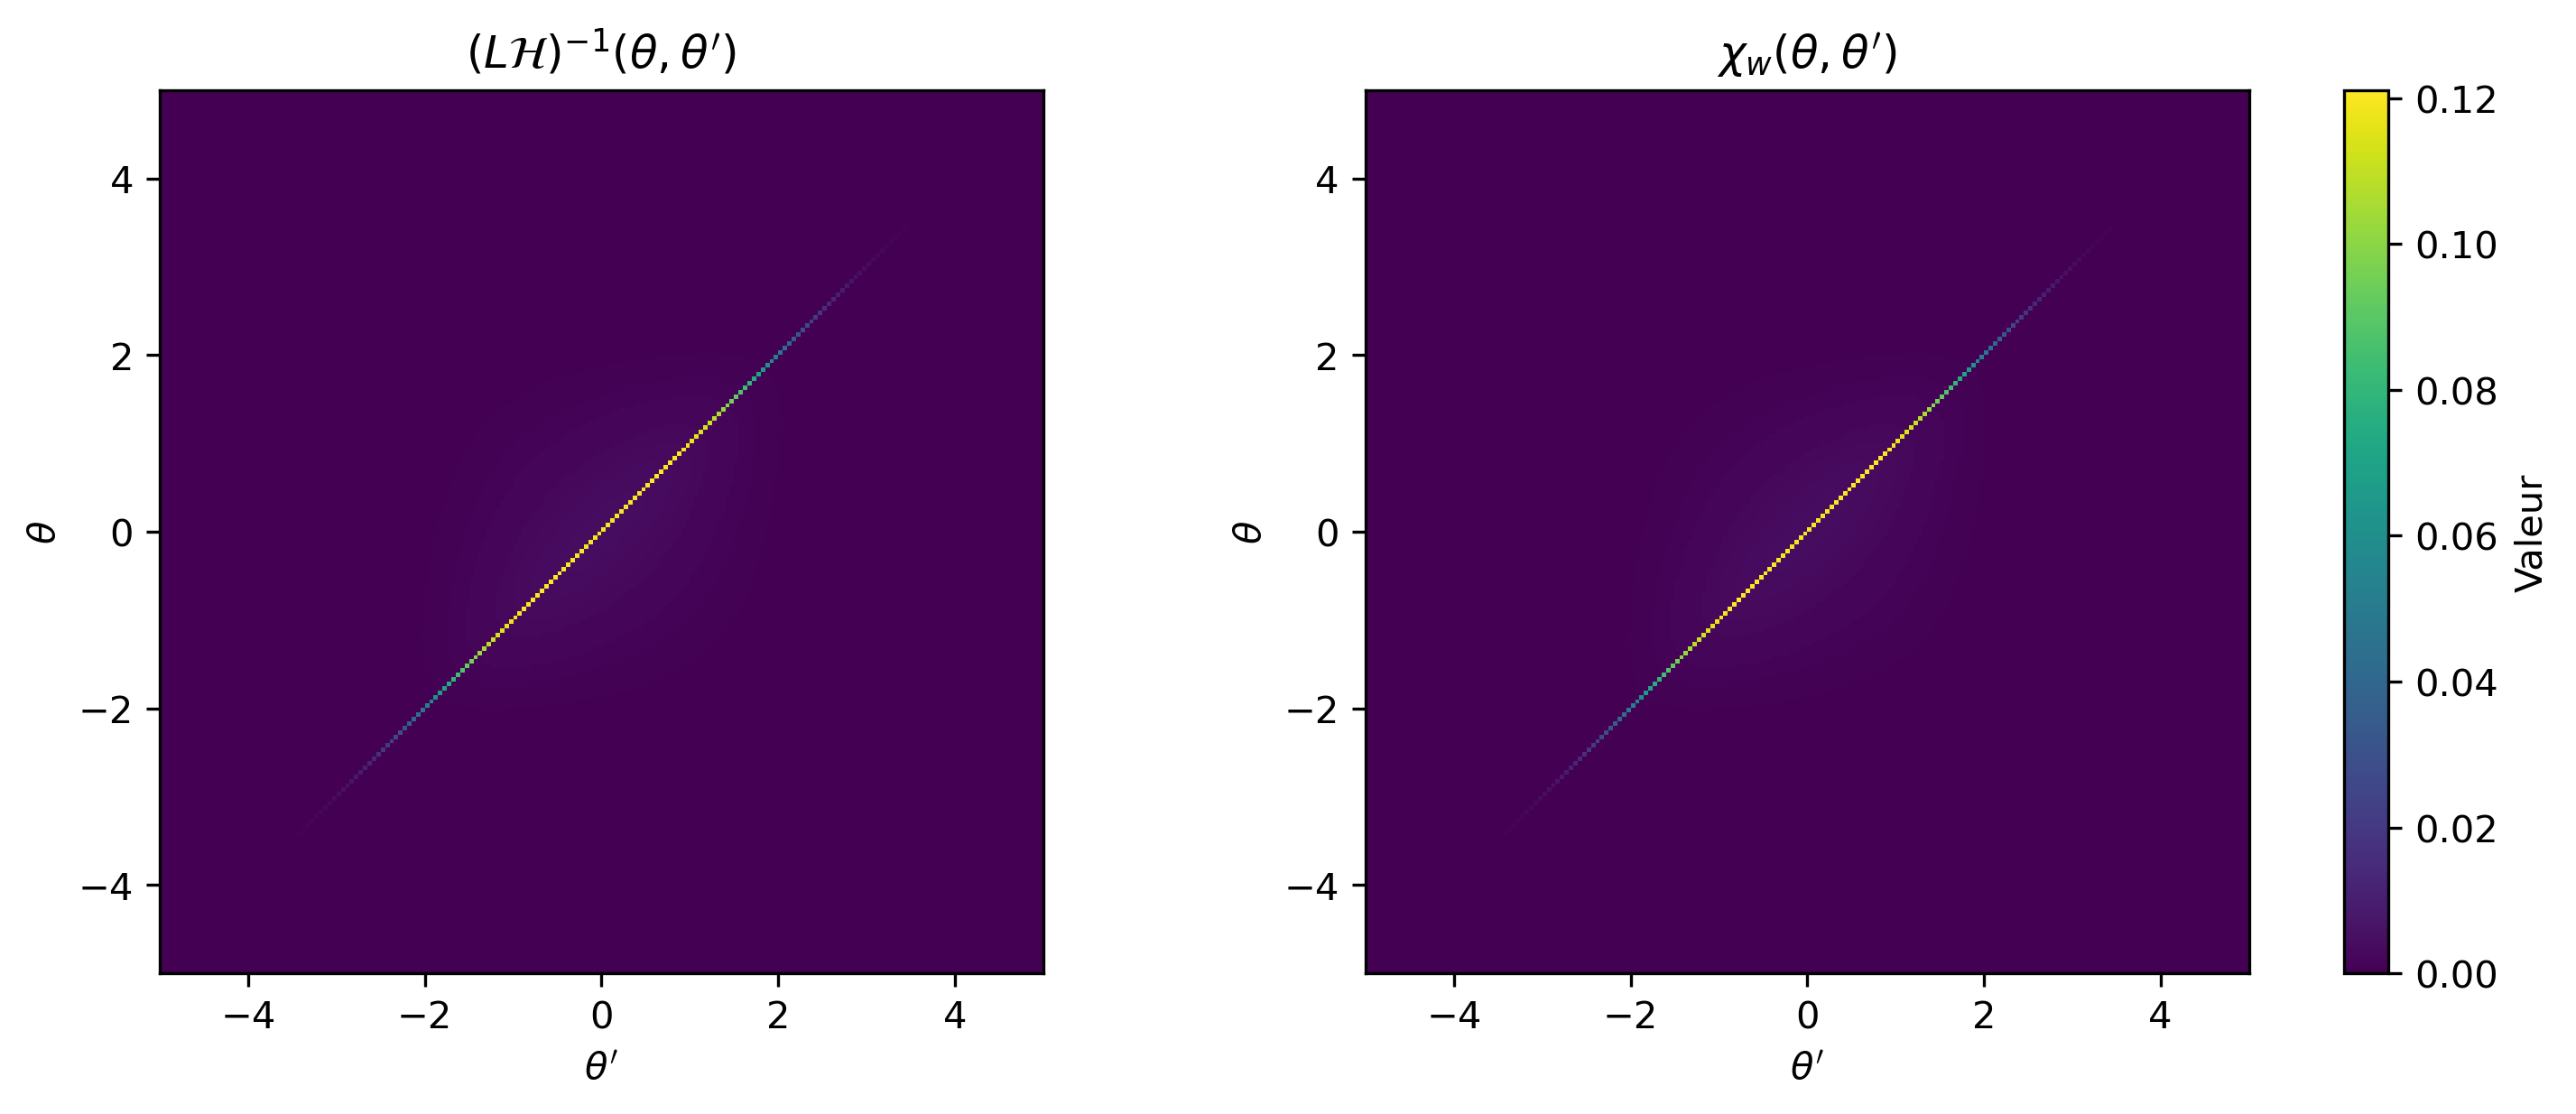
\includegraphics[width=1\textwidth]{figures/04_GGE_Fluctuation/heatmaps_2.png}
    \caption{Vérification numérique dans le régime thermodynamique. Gauche : $(L\mathcal{H})^{-1}$ par inversion de la courbure. Droite : \(\chi_w\) par dérivée fonctionnelle.}
    \label{fig:chi_thermodynamique}
\end{figure}

\paragraph{Conclusion.}

Nous avons vérifié la formule \eqref{chap:fluctu:eq:fluctuations.10} de deux manières. D’une part, en évaluant directement à un {\em poids spectral} $w$ fixé $(L\mathcal{H})^{-1}$; d’autre part, en calculant la différentielle de la distribution de rapidité par rapport au poids spectral \(\chi_w\), c’est-à-dire  en appliquant le principe de fluctuation–réponse. Pour le {\em poids spectral} et les paramètres considérés, les deux approches donnent des résultats numériques concordants, ce qui constitue une validation de la formule \eqref{chap:fluctu:eq:fluctuations.10}.

%Cette vérification confirme que, dans le régime thermodynamique, la structure variationnelle de l’entropie de \gls{YY} encode entièrement les fluctuations et les réponses spectrales du système. Il s’agit d’un test non trivial du principe de fluctuation–réponse appliqué aux systèmes intégrables.

\medskip

Dans un second temps, il est naturel de vouloir tester ce principe pour différentes formes du {\em poids spectral} $w$. Dans le cas général du \gls{GGE}, $w$ appartient à un espace de dimension infinie. Afin de réduire cette complexité, nous nous restreignons à une sous-famille à deux paramètres, en nous plaçant dans le cadre de l’équilibre thermique. Ce choix permet de comparer explicitement les fluctuations de grandeurs thermodynamiques macroscopiques, telles que le nombre total de particules et l’énergie cinétique.




%\section{Lien entre dérivée fonctionnelle et réponse linéaire aux facteurs de Lagrange}

\subsubsection{Vérification numérique thermique :  énergie et nombre de particules}

Nous testons à présent notre expression des fluctuations dans le cas particulier de l'équilibre thermique. Le sous-système est supposé en contact avec un bain à température \( T \) et potentiel chimique \( \mu \).
%Le poids spectral prend alors la forme canonique :
%\(
%w(\theta) = \beta \varepsilon(\theta) - \beta \mu,
%\)
%avec \( \beta = 1 / (k_B T) \) et \( \varepsilon(\theta) \) l’énergie (par exemple \( m\theta^2/2 \) pour des particules libres).

%\subparagraph{Paramètres fixés.}
%Dans le cas de l’équilibre thermique usuel (ensemble de Gibbs), seules deux charges sont conservées : le {\bf nombre total de particules} \( \operator{\mathcal{Q}}[f_0] \) et l’{\bf énergie totale} \( \operator{\mathcal{Q}}[f_2] \). Cela correspond au choix suivant :
%\begin{align*}
%	f_0(\theta) &= 1, \quad &&\text{(densité de particules)} \\
%	f_2(\theta) &= \frac{1}{2}m \theta^2, \quad &&\text{(densité d’énergie $\varepsilon$)}
%\end{align*}
%les coefficients de Lagrange associés sont :
%\begin{align*}
%	\beta_0 &= -\beta \mu, \quad &&\text{(potentiel chimique)} \\
%	\beta_2 &= \beta, \quad &&\text{(inverse de la température)},
%\end{align*}
%avec $\beta = 1 / ( k_B T )$ et  $k_B$ constante de Boltzmann.
%
%\medskip
%
%\paragraph{Calcul de la matrice hermitienne.}
%
%On reprend ici le formalisme de l’équation \eqref{chap4:eq.w_fi}, dans lequel le poids spectral s’écrit comme une combinaison linéaire :
%\begin{eqnarray}\label{chap4:eq.w.1}
%	w(\theta) & = & \beta_0 f_0(\theta) + \beta_2 f_2(\theta),
%\end{eqnarray}
%où \( f_0(\theta) = 1 \) et $f_2(\theta) = \frac{1}{2}m \theta^2,$ sont les densités locales associées aux charges conservées , fixeé et $\beta_0$ et $\beta_2$ en imposant une température \(T\) et un potentiel chimique \(\mu\).
%
%Dans les équations \eqref{chap2:eq:gamma.1} et \eqref{chap2:eq:t.1}, nous avons défini les grandeurs adimensionnées, le {\bf paramètre de Lieb} $\gamma$ et la {\bf température réduite} $t$, telles que :
%\begin{eqnarray*}
%	\gamma = \frac{m g}{\hbar^2 n}, \quad t = \frac{\hbar^2}{m \beta g^2}.
%\end{eqnarray*}
%
%\subparagraph{Paramètres fixes.}
%Nous travaillons avec $\hbar = m = k_B = 1$, et nous choisissons $L = 100$ et $g = 1$.
%
%\subparagraph{Paramètres variables.}
%La température $T$ est alors donnée par la température réduite $t$, et la densité linéaire $n$ est inversement proportionnelle au paramètre adimensionné $\gamma$.


%\paragraph{Calcul de la matrice hermitienne.}
%
%Les densités locales $f_i$ sont fixées. Pour spécifier le {\em poids spectral} $w$, on choisit les coefficients de Lagrange $\beta_0$ et $\beta_2$ en imposant une température \(T\) et un potentiel chimique \(\mu\).
%
%\medskip
%
%Dans les équations \eqref{chap2:eq:gamma.1} et \eqref{chap2:eq:t.1}, nous avons défini les grandeurs adimensionnées, le {\bf paramètre de Lieb} $\gamma$ et la {\bf température réduite} $t$, telles que :
%\begin{eqnarray*}
%	\gamma = \frac{m g}{\hbar^2 n}, \quad t = \frac{\hbar^2}{m \beta g^2}.
%\end{eqnarray*}



%La densité linéaire \( n \) ne paramétrise pas directement le poids spectral $w$ \eqref{chap4:eq.w.1}, mais est liée au potentiel chimique \(\mu\) via :
%\[
%	L n = \braket{\operator{\mathcal{Q}}[f_0]}_w.
%\]
%C’est ainsi que les simulations numériques seront effectuées en utilisant $\gamma$ et $t$.

%\subparagraph{Paramètres variables.}
%Avec ces conventions, la densité linéaire $n$ est reliée directement au paramètre $\gamma$, tandis que la température physique $T$ est déterminée par la température réduite $t$. Ainsi, dans l’équation~\eqref{chap4:eq.w.1}, les fonctions $f_i(\theta)$ sont fixées, et ce sont les coefficients $\beta_i$ qui s’ajustent en fonction des paramètres adimensionnés $\gamma$ et $t$, c’est-à-dire en fonction des conditions thermodynamiques imposées.



\paragraph{Calcul de la matrice hermitienne.}

Dans la section~\ref{chap4:sec:TBA}, nous avons présenté les différentes étapes de la résolution numérique de l’équation de \gls*{TBA}.
Nous reprenons ici le formalisme de l’équation~\eqref{chap4:eq.w_fi}, dans lequel le poids spectral s’écrit comme une combinaison linéaire :
\begin{equation}\label{chap4:eq.w.1}
	w(\theta) = \beta_0 f_0(\theta) + \beta_2 f_2(\theta),
\end{equation}
où $f_0(\theta) = 1$ et $f_2(\theta) = \tfrac{1}{2} m \theta^2$ correspondent aux densités locales associées aux charges conservées.
Les coefficients $\beta_0 = - \beta \mu $ et $\beta_2 = \beta (= (k_B T)^{-1})$ sont fixés de manière à imposer une température $T$ et un potentiel chimique $\mu$.

\medskip

Le \textbf{paramètre de Lieb} et la \textbf{température réduite}, définis respectivement en~\eqref{chap2:eq:gamma.1} et~\eqref{chap2:eq:t.1},
\begin{equation*}
	\gamma = \frac{m g}{\hbar^2 n},
	\qquad
	t = \frac{\hbar^2}{m \beta g^2},
\end{equation*}
permettent également de paramétrer le couple $(T,\mu)$ (voir section~\ref{chap4:sec:TBA}).

% \subparagraph{Paramètres fixes.}
% Dans toute la suite, nous travaillons avec les conventions $\hbar = m = k_B = 1$, ainsi que $L = 100$ et $g = 1$.

% \medskip

% \subparagraph{Choix des paramètres.}
% Nous considérons le point
% \begin{equation*}
% 	\gamma = 0.02,
% 	\qquad
% 	t = 70 ,
% \end{equation*}
% qui est représenté par un \textbf{point rouge} dans le diagramme de phase du modèle de \gls{LL}, présenté en figure~\ref{chap:4:fig:diagr}.

\begin{tcolorbox}[colback=blue!5!white,colframe=blue!75!black,title=Remarque]
On rappelle que le paramètre de Lieb \(\gamma\) caractérise la force d'interaction relative entre les particules, tandis que la température réduite \(t\) quantifie l'importance des effets thermiques par rapport aux interactions. En variant ces deux paramètres, on explore différents régimes physiques du système.
\end{tcolorbox}

\begin{tcolorbox}[colback=blue!5!white,colframe=blue!75!black,title=Remarque]
Dans cette continuité, nous allons définir des unités naturelles adaptées au système étudié. Ces unités facilitent l'interprétation physique des résultats numériques en les reliant directement aux grandeurs expérimentales.

\subparagraph{Conversion vers les unités réelles.}
Mais avant pour faciliter la comparaison avec les expériences, nous allons définir des unités caractéristiques:

\begin{eqnarray}
\ell_0 &= &  \frac{\hbar^2}{m g}, \quad \text{(longueur)}\\
\tau_0 &= &  \frac{m \ell_0^2}{\hbar},  \quad \text{(temps)}\\
E_0 &= & \frac{\hbar^2}{m L_0^2}, \quad \text{(énergie)}\\
T_0 &=&\frac{E_0}{k_B}, \quad \text{(température)}.
\end{eqnarray}

Mes résultats numériques sont exprimés en unités naturelles adimensionnées. Pour revenir aux valeurs réelles, il suffit de les multiplier par les unités caractéristiques définies ci-dessus.

% Ainsi, les paramètres naturels peuvent être convertis en unités réelles par
% \[
% x_\text{réel} = L_0 \, x_\text{nat}, 
% \qquad
% t_\text{réel} = T_0 \, t_\text{nat}, 
% \qquad
% T_\text{réel} = T_\text{nat} \, T_\text{nat},
% \]
% permettant de comparer directement nos résultats numériques avec les expériences.
\end{tcolorbox}	


\subparagraph{Paramètres fixes.}
Dans toute la suite, nous travaillons avec les conventions naturelles
\(\hbar = m = k_B = 1\), ainsi qu'avec
\begin{equation*}
L = 10, \qquad g = 1.
\end{equation*}

\medskip



\subparagraph{Choix des paramètres.}
Nous considérons le point
\begin{equation*}
    \gamma = 0.02,
    \qquad
    t = 70,
\end{equation*}
qui est représenté par un \textbf{point rouge} dans le diagramme de phase du modèle de \gls{LL}, présenté en figure~\ref{chap:4:fig:diagr}.


\begin{tcolorbox}[colback=blue!5!white,colframe=blue!75!black,title=Remarque]
Les paramètres choisis ne sont pas arbitraires : ils sont proches des régimes expérimentaux que nous considérons. 
La taille du sous-système \(L\) est en unité réelle de $22\,\mu m$, la densité linéaire \(n\) est de l'ordre de $23\,\mu m^{-1}$ et la température \(T\) est d'environ $81\,nK$.
\end{tcolorbox}

% \medskip

% \subparagraph{Conversion vers les unités réelles.}
% Pour relier ces valeurs aux grandeurs physiques réelles, on définit les unités naturelles :
% \[
% \begin{aligned}
% L_0 &= \frac{\hbar^2}{m g_\text{réel}}, &\text{(longueur)}\\
% T_0 &= \frac{m L_0^2}{\hbar}, &\text{(temps)}\\
% E_0 &= \frac{\hbar^2}{m L_0^2}, &\text{(énergie)}\\
% T_\text{nat} &= \frac{E_0}{k_B}, &\text{(température)}
% \end{aligned}
% \]

% Ainsi, les paramètres naturels peuvent être convertis en unités réelles par
% \[
% x_\text{réel} = L_0 \, x_\text{nat}, 
% \qquad
% t_\text{réel} = T_0 \, t_\text{nat}, 
% \qquad
% T_\text{réel} = T_\text{nat} \, T_\text{nat},
% \]
% permettant de comparer directement nos résultats numériques avec les expériences.





\medskip

À partir de ce paramètre, et suivant la même procédure numérique que dans la sous-section précédente, on obtient la distribution de rapidité à l'équilibre
\(\braket{\operator{\rho}(\theta)}_w \equiv \rho_{\mathrm{eq}}(\theta)\), ainsi que les composantes de l’inverse de l’opérateur hessien \((L\mathcal{H})^{-1}\) : la contribution diagonale sans interaction \((L\mathcal{D})^{-1}\) (Fig.~\ref{chap:4:fig:fluctu_diag}) et la contribution non locale issue des interactions \(\mathcal{B}/L\) (Fig.~\ref{chap:4:fig:fluctu_B}).

\medskip

Plus précisément, dans la figure~\ref{chap:4:fig:fluctu_diag}, on représente
\begin{eqnarray*}
	\frac{\mathcal{D}^{-1}(\theta, \theta')}{\delta(\theta - \theta')} \quad  \left( =  \rho_{s, \mathrm{eq}}(\theta) \, \nu_{\mathrm{eq}}(\theta) \, (1 - \nu_{\mathrm{eq}}(\theta)) \right),
\end{eqnarray*}
la fonction delta dans \eqref{chap:fluctu:eq:irreg.inv} étant approximée numériquement par un pas de discrétisation, la matrice \(\mathcal{D}^{-1}\) est proportionnelle à ce pas.

\medskip

Enfin, en faisant varier $t$ (\ie la température \(T\)), on répète l'ensemble des calculs précédents.
Les régimes ainsi obtenus sont indiqués par des {\bf points bleus} dans le diagramme de phase (figure~\ref{chap:4:fig:diagr}).



\paragraph{Corrélation des observables thermodynamiques.}

\medskip
Conformément à l’équation~\eqref{chap4:eq.cumulant.distr.q.10}, nous calculons les fluctuations du nombre total de particules ainsi que celles de l’énergie totale, respectivement données par :
\begin{eqnarray}
	C_w[f_0,f_0]  & = & L^2 \iint d\theta\, d\theta'\; f_0(\theta)\, (L\mathcal{H})^{-1}(\theta , \theta')\, f_0(\theta') ,\\
	C_w[f_2,f_2]  & = & L^2 \iint d\theta\, d\theta'\; f_2(\theta)\,(L\mathcal{H})^{-1}(\theta , \theta')\, f_2(\theta').
\end{eqnarray}

Pour chaque régime simulé (correspondant aux {\bf points bleus} et {\bf rouge} sur la figure~\eqref{chap:4:fig:diagr}), nous évaluons numériquement les quantités \( C_w[f_0,f_0] \) et \( C_w[f_2,f_2] \), qui représentent les fluctuations extensives des observables associées aux charges \( \operator{Q}_0 \) (nombre de particules) et \( \operator{Q}_2 \) (énergie cinétique).

\medskip

Ces résultats sont représentés par des {\bf points rouges} dans la figure~\ref{chap:4:fig.fluctu.A_com}, illustrant l’évolution des fluctuations en fonction du régime thermodynamique du sous-système.


\paragraph{Susceptibilité des observables thermodynamiques.}

\medskip
En parallèle, pour chaque régime simulé (correspondant aux {\bf points bleus} et {\bf rouge} de la figure~\eqref{chap:4:fig:diagr}), et conformément à l’équation~\eqref{chap4:eq.moment.distr.q.10}, nous calculons les moyennes des charges associées au nombre total de particules et à l’énergie cinétique totale, données respectivement par :
\begin{eqnarray}
	\braket{\operator{\mathcal{Q}}[f_0]}_w & = & L \int d\theta\; f_0(\theta)\, \braket{\operator{\rho}(\theta)}_w,\\
	\braket{\operator{\mathcal{Q}}[f_2]}_w & = & L \int d\theta\; f_2(\theta)\, \braket{\operator{\rho}(\theta)}_w.
\end{eqnarray}

\medskip

Nous souhaitons ensuite évaluer les susceptibilités thermodynamiques définies par :
\begin{eqnarray}
	\chi_w[f_i, f_i] & = & - \left. \frac{\partial \braket{\operator{\mathcal{Q}}[f_i]}_w}{\partial \beta_i} \right)_{\beta_{j \neq i} \text{ fixés}}.
\end{eqnarray}

Pour cela, nous procédons à une variation infinitésimale du poids spectral $w$ :

\begin{itemize}[label =$\bullet$]
	\item Une variation infinitésimale $\epsilon_\mu$ du potentiel chimique $\mu$ correspond à une perturbation du poids spectral de la forme :
	\[
	w \rightarrow w - \beta \epsilon_\mu f_0.
	\]
	On résout alors numériquement les équations \gls{TBA} pour ce nouveau poids, afin de calculer :
	\[
	\braket{\operator{\mathcal{Q}}[f_0]}_{w - \beta \epsilon_\mu f_0}.
	\]

	\item On effectue ensuite une variation infinitésimale $\epsilon_\beta$ de l’inverse de la température, de sorte que la combinaison \( (\beta + \epsilon_\beta)(\mu + \epsilon_\mu) = \beta \mu \) reste constante, maintenant ainsi $\beta_0$ fixe. Cela conduit à une variation du poids spectral de la forme :
	\[
	w \rightarrow w + (\beta + \epsilon_\beta)(- \epsilon_\mu f_0 + f_2).
	\]
	On résout à nouveau les équations TBA pour obtenir :
	\[
	\braket{\operator{\mathcal{Q}}[f_2]}_{w + (\beta + \epsilon_\beta)(- \epsilon_\mu f_0 + f_2)}.
	\]
\end{itemize}

\medskip

Ces simulations permettent d’estimer numériquement les susceptibilités :
\begin{eqnarray}
	\chi_w[f_0, f_0]	 & \approx & \frac{\braket{\operator{\mathcal{Q}}[f_0]}_{w - \beta \epsilon_\mu f_0} - \braket{\operator{\mathcal{Q}}[f_0]}_w}{\beta \epsilon_\mu},	\\
	\chi_w[f_2, f_2]	 & \approx & - \frac{\braket{\operator{\mathcal{Q}}[f_2]}_{w + (\beta + \epsilon_\beta)(- \epsilon_\mu f_0 + f_2)} - \braket{\operator{\mathcal{Q}}[f_2]}_w}{\epsilon_\beta}.
\end{eqnarray}

\medskip

Ces approximations numériques sont représentées par des {\bf points bleus} dans la figure~\eqref{chap:4:fig.fluctu.A_com}, et permettent de comparer les résultats issus de la dérivée fonctionnelle avec ceux provenant de la réponse directe à une perturbation du poids spectral.



%Conformément à l'équation \eqref{chap4:eq.moment.distr.q.10} la densité linéaire $n$

%Pour explorer différents  zone du diagramme de phase du modèle de Lieb-Liniger



%\paragraph{Cas du nombre de particules.}
%On choisit la fonction test \( f_{\operator{Q}}(\theta) = 1 \), ce qui définit la charge associée :
%\[
%\operator{Q} = \operator{\mathcal{Q}}[1] = L \int d\theta\, \operator{\rho}(\theta).
%\]
%Son facteur de Lagrange / potentiel conjugué dans \( w(\theta) \) est simplement :
%\[
%w(\theta) \supset -\beta \mu \cdot 1.
%\]
%La susceptibilité  et les corrélations associée sont égaux:
%\[
%\chi_w[{\operator{Q},\operator{Q}}] \doteq \left . \frac{\partial \langle \operator{Q} \rangle_w}{\partial (\beta \mu)} \right)_\beta  = L^2 \iint d\theta\, d\theta'\, C_w(\theta, \theta') \doteq C_w(f_{\operator{Q}}, f_{\operator{Q}}).
%\]
%
%\paragraph{Cas de l’énergie.}
%On prend maintenant \( f_{\operator{H}}(\theta) = \varepsilon(\theta) \), l’énergie spectrale (ici par ex. \( \theta^2/2 \) pour des particules libres), ce qui donne :
%\[
%\operator{H} = \operator{\mathcal{Q}}[\varepsilon] = L \int d\theta\, \varepsilon(\theta)\, \operator{\rho}(\theta),
%\]
%et facteur de Lagrange / potentiel conjugué  est simplement \( \beta \varepsilon(\theta) \), avec :
%\[
%w(\theta) \supset \beta \varepsilon(\theta).
%\]
%On en déduit la susceptibilité thermique :
%\[
%\chi_{\operator{H},\operator{H}} \doteq -\left.\frac{\partial \langle \operator{H} \rangle_w}{\partial \beta} \right)_{\beta \mu}  = L^2 \iint d\theta\, d\theta'\, \varepsilon(\theta)\, C_w(\theta, \theta')\, \varepsilon(\theta') \doteq C_w(f_{\operator{H}}, f_{\operator{H}}).
%\]

%\paragraph{Évaluation numérique.}

%On fais les calcule des correlation pour $\gamma = g/n $ fixé à ?? et $t = 1/(\beta g^2)$ entre ?? et ??.Les points correspondants sont représentés en bleu sur un diagramme de phase du modèle de Lieb-Liniger (voir Fig.~\ref{fig:diag}).

%Ce même diagramme contient également un point rouge correspondant à \( t = ?? \). Les fluctuations associées à ce point sont représentées en niveaux de couleur sur un graphique 2D (voir Fig.~\ref{fig.fluctu.A})

%Les corrélations de \( \rho(\theta) \) sont calculées numériquement pour un couplage \(\gamma = g/n\) fixé, et une température réduite \( t = 1 / (\beta g^2) \) variant dans un intervalle donné. Les points correspondants sont indiqués en \textbf{bleu} dans le diagramme de phase du modèle de Lieb-Liniger (Fig.~\ref{fig:diag}).
%
%Dans ce même diagramme, un \textbf{point rouge} correspond à des conditions fixes (\(T = 60~\mathrm{nK}\), \( \mu = 27~\mathrm{nK} \)), pour lesquelles la carte des fluctuations \( \delta \rho \) est représentée en niveaux de couleur (Fig.~\ref{fig.fluctu.A}).


%\begin{figure}[H]
%	\centering
%	\begin{subfigure}[b]{0.25\textwidth}
%		
\includegraphics[width=\textwidth]{Figures/04_GGE_Fluctuation/diagram.png}
%		\caption{Diagramme de phase du modèle de Lieb-Liniger.}
%		\label{chap:4:fig:diagr}
%	\end{subfigure}
%	\hfill
%	\begin{subfigure}[b]{0.3\textwidth}
%		
\includegraphics[width=\textwidth]{Figures/04_GGE_Fluctuation/diag_fluctu_1.png}
%		\caption{ \( \mathcal{D}^{-1}(\theta, \theta)/\delta(\theta, \theta) \).}
%		\label{chap:4:fig.fluctu.A}
%	\end{subfigure}
%	\hfill
%	\begin{subfigure}[b]{0.4\textwidth}
%		
\includegraphics[width=\textwidth]{Figures/04_GGE_Fluctuation/fluctu_1.png}
%		\caption{ \( \mathcal{B}(\theta, \theta') \).}
%		\label{chap:4:fig.fluctu.A}
%	\end{subfigure}
%	\caption{(a) Diagramme de phase du modèle de Lieb-Liniger à l’équilibre thermique. Différents régimes asymptotiques sont séparés par des transitions progressives. Les points bleus représentent les fluctuations calculées numériquement pour différentes températures. Les coordonnées sont données par \( \gamma = \frac{m g}{\hbar^2 n} \) et \( t = \frac{k_B T}{m g^2/\hbar^2} \). On Représenter les régimes choisir pour les simulation en point blue ( à \( \gamma = 10^{-1.7} \) constant et en rouge pour \( t = 89.125 \) un point représenté en (b) et (c). (b) Representation de diagolale $\mathcal{D}^{-1}(\theta, \theta)/\delta(\theta, \theta)$ et (c) Représentation en niveaux de couleur de la partie régulière $\mathcal{B}$ des fluctuations \( \delta \rho \) pour \( t = 89.125 \) et \( \gamma = 10^{-1.7} \) (point rouge dans (a)).}
%	\label{chap:4:fig:diag_fig}
%\end{figure}
%
%\begin{figure}[H]
%    \centering
%    \begin{subfigure}[b]{0.25\textwidth}
%        
\includegraphics[width=\textwidth]{Figures/04_GGE_Fluctuation/diagram.png}
%        \caption{Diagramme de phase du modèle de Lieb-Liniger à l’équilibre thermique.}
%        \label{chap:4:fig:diagr}
%    \end{subfigure}
%    \hfill
%    \begin{subfigure}[b]{0.3\textwidth}
%        
\includegraphics[width=\textwidth]{Figures/04_GGE_Fluctuation/diag_fluctu_1.png}
%        \caption{Diagonale \( \mathcal{D}^{-1}(\theta, \theta)/\delta(\theta, \theta) \) des fluctuations.}
%        \label{chap:4:fig:fluctu_diag}
%    \end{subfigure}
%    \hfill
%    \begin{subfigure}[b]{0.4\textwidth}
%        
\includegraphics[width=\textwidth]{Figures/04_GGE_Fluctuation/fluctu_1.png}
%        \caption{Représentation en niveaux de couleur de la partie régulière \( \mathcal{B}(\theta, \theta') \) des fluctuations \( \delta \rho \) pour \( t = 89.125 \) et \( \gamma = 10^{-1.7} \).}
%        \label{chap:4:fig:fluctu_B}
%    \end{subfigure}
%    \caption{(a) Diagramme de phase du modèle de Lieb-Liniger, avec les différents régimes asymptotiques séparés par des transitions progressives. Les points bleus indiquent les valeurs des fluctuations calculées numériquement pour différentes températures. Les coordonnées sont données par \( \gamma = \frac{m g}{\hbar^2 n} \) et \( t = \frac{k_B T}{m g^2/\hbar^2} \). Le point rouge correspond aux paramètres utilisés pour les sous-figures (b) et (c). (b) Diagonale de \( \mathcal{D}^{-1}(\theta, \theta)/\delta(\theta, \theta) \). (c) Partie régulière \( \mathcal{B}(\theta, \theta') \) des fluctuations \( \delta \rho \).}
%    \label{chap:4:fig:diag_fig}
%\end{figure}

\begin{figure}[H]
    \centering
    \begin{subfigure}[b]{0.25\textwidth}
        
\includegraphics[width=\textwidth]{Figures/04_GGE_Fluctuation/diagram.png}
        \caption{Diagramme de phase du modèle de Lieb-Liniger.}
        \label{chap:4:fig:diagr}
    \end{subfigure}
    \hfill
    \begin{subfigure}[b]{0.3\textwidth}
        
\includegraphics[width=\textwidth]{Figures/04_GGE_Fluctuation/diag_fluctu_1.png}
        \caption{\( \mathcal{D}^{-1}(\theta, \theta)/\delta(\theta, \theta) \).}
        \label{chap:4:fig:fluctu_diag}
    \end{subfigure}
    \hfill
    \begin{subfigure}[b]{0.4\textwidth}
        
\includegraphics[width=\textwidth]{Figures/04_GGE_Fluctuation/fluctu_1.png}
        \caption{\( \mathcal{B}(\theta, \theta') \).}
        \label{chap:4:fig:fluctu_B}
    \end{subfigure}
    \caption{
    (a) Diagramme de phase du modèle de \acrlong{LL} à l’équilibre thermique. Différents régimes asymptotiques sont séparés par des transitions progressives. Les points bleus représentent les fluctuations calculées numériquement pour différentes températures. Les coordonnées sont données par \( \gamma = \frac{m g}{\hbar^2 n} \) et \( t = \frac{k_B T}{m g^2/\hbar^2} \). Les régimes choisis pour les simulations sont indiqués par les points bleus (\( \gamma = 0.02 \) constant) et le point rouge correspond à \( t = 70 \), utilisé dans les sous-figures (b) et (c).
    (b) Représentation de la diagonale \( \mathcal{D}^{-1}(\theta, \theta)/\delta(\theta, \theta) \).
    (c) Représentation en niveaux de couleur de la partie régulière \( \mathcal{B} \) des fluctuations de\( \delta \rho \) pour \( t = 70 \) et \( \gamma = 0.02 \) (point rouge dans (a)).
    }
    \label{chap:4:fig:diag_fig}
\end{figure}



\paragraph{Comparaison avec les dérivées thermodynamiques.}

Les résultats obtenus à partir de l’analyse quadratique de l’action (fluctuations de \( \rho \)) sont comparés aux fluctuations extraites directement par différentiation des observables thermodynamiques \( \langle \operator{Q} \rangle_w \) et \( \langle \operator{H} \rangle_w \). Ces comparaisons sont présentées dans la Fig.~\ref{chap:4:fig.fluctu.A_com} et révèlent une excellente concordance. On le quantifie avec :
\begin{eqnarray*}
	\left \vert \frac{C_w[f_0,f_0] -  \chi_w[f_0,f_0]}{C_w[f_0,f_0]} \right \vert < 0.004\% , \quad \left \vert \frac{C_w[f_2,f_2] -  \chi_w[f_2,f_2]}{C_w[f_2,f_2]} \right \vert < 0.14 \%.
\end{eqnarray*}

%Les résultats obtenus à l’aide de cette méthode thermodynamique sont comparés à ceux issus du calcul direct des fluctuations de \( \rho \). Ces comparaisons sont représentées sur la Fig.~\ref{fig.fluctu.A_com}, et montrent une excellente concordance entre les deux approches.

\begin{figure}[H]
	\centering
	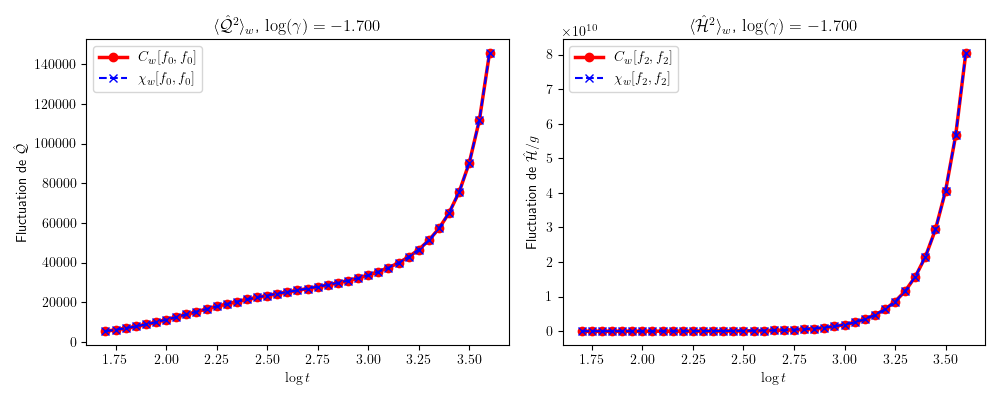
\includegraphics[width=1\textwidth]{figures/04_GGE_Fluctuation/fluctuations_plot_log_gamma=-1.700.png}
	%
\includegraphics[width=1\textwidth]{Figures/04_GGE_Fluctuation/fluctuations_relativ_plot_log_gamma=-1.342.png}
	\caption{Comparaison numérique entre  $C_w[f_0,f_0]$ et $\chi_w[f_0,f_0]$ et entre $C_w[f_2,f_2]$ et $\chi_w[f_2,f_2]$.}
	\label{chap:4:fig.fluctu.A_com}
\end{figure}



\section*{Conclusion}

Dans ce chapitre, nous avons étudié les fluctuations de la distribution de rapidité dans les états \gls{GGE}, en mettant en lumière le lien fondamental entre corrélations et réponse linéaire.

\medskip

Nous avons d’abord introduit le formalisme général des \gls{GGE}, dans lequel les observables macroscopiques sont dérivées fonctionnellement du potentiel conjugué $w(\theta)$. Dans ce cadre, nous avons montré que la matrice de susceptibilité spectrale $\chi_w(\theta , \theta')$ décrit à la fois la réponse linéaire de la densité spectrale moyenne à une perturbation infinitésimale du potentiel et les corrélations entre fluctuations de la densité, conformément au principe de \emph{fluctuation-réponse}. En utilisant ce lien, nous avons vu que nous pouvons  \emph{échantillonner \gls{GGE}}.

\medskip

Nous avons ensuite approfondi l’étude de la limite thermodynamique, où les fluctuations autour de l’état d’équilibre deviennent gaussiennes. Dans cette approximation, les susceptibilités s’expriment comme l’inverse de la courbure fonctionnelle de l’entropie de Yang-Yang, formalisée par l’opérateur hessien $\mathcal{H}^{(\mathcal{S}_{YY})}$. Nous avons donné une formulation explicite de cet opérateur, ainsi que de sa matrice inverse.

\medskip

Enfin, nous avons relié ces objets locaux à des susceptibilités globales via une projection sur les fonctions test $f_i(\theta)$, en considérant le poids spectral $w(\theta)$ comme une combinaison linéaire des charges $\operator{Q}_i$ . Ce formalisme nous a permis d’interpréter la dérivée de l’observable $\langle \operator{Q}_i \rangle_w$ par rapport au multiplicateur de Lagrange $\beta_i$ comme une dérivée fonctionnelle projetée de la matrice $\chi_w(\theta , \theta')$, et d’en valider la structure par une comparaison numérique explicite pour l’énergie et le nombre de particules.

\medskip

Nous avons vérifié numériquement la validité de notre formule des fluctuations (eq~\eqref{chap:fluctu:eq:fluctuations.10}), ce qui confirme son exactitude et sa pertinence dans le cadre du formalisme développé.


%\paragraph{🔸 Remarque sur les corrélations globales.}
%Dans les deux cas, les fluctuations totales \( \langle \delta N^2 \rangle \), \( \langle \delta E^2 \rangle \), ou croisées \( \langle \delta E\, \delta N \rangle \), sont données par les projections :
%\[
%\langle \delta Q_i\, \delta Q_j \rangle = \chi_{ij} = L^2 \iint d\theta\, d\theta'\, f_i(\theta)\, \chi(\theta, \theta')\, f_j(\theta').
%\]
%Cela généralise l’idée de la **formule de fluctuation-réponse** : la réponse à un potentiel conjugué est gouvernée par les corrélations spontanées du système au point d’équilibre.
%
%\paragraph{✅ Conclusion.}
%Pour toute charge \( \mathcal{Q}[f] = L \int f(\theta)\, \operator{\rho}(\theta)\, d\theta \), on a :
%\[
%\boxed{
%\chi_{f,f} = -\frac{\partial \langle \mathcal{Q}[f] \rangle}{\partial \lambda} = L^2 \iint d\theta\, d\theta'\, f(\theta)\, \chi(\theta, \theta')\, f(\theta'),
%}
%\]
%où \( \lambda \) est le coefficient dans \( w(\theta) = \lambda f(\theta) \).
%




%------------------------
%
%
%\section{Fonction correlation du nombre d'atomes et de l'énergie}
%
%
%Il est maintenant pertinent de tester notre expression des fluctuations. On fait l'hypothèset que le système est en équilibre thermique caractérisé par la températeur $T$ et le potentiel chimoque $\mu$.
%
%La valeur propre $\mathcal{N}[\rho]$ (resp $\mathcal{E}[\rho]$) de opérateur nombre d'atomes $\operator{\mathcal{N}}$ (resp énergie. $\operator{\mathcal{E}}$) et assiciés aux configuration liès à la distribution de rapidité $\rho$ s'écrit (avec comme combention la masse des atomes $k_B = \hbar = m =1$)
%
%\begin{eqnarray*}
%	\mathcal{N}[\rho] & = & L \int d \theta \rho(\theta),\\
%	\mathcal{E}[\rho] & = & 	\frac{L}2 \int d \theta  \theta^2 \rho(\theta).
%\end{eqnarray*}
%
%Les corrélation associèes s'est
%\begin{eqnarray*}
%	C_{\operator{\mathcal{N}},\operator{\mathcal{N}}} & = &  L^2 \int d\theta_a \int d\theta_b \, \langle \delta \rho(\theta_a) \delta \rho(\theta_b) \rangle, \\
%	C_{\operator{\mathcal{E}},\operator{\mathcal{E}}} & = &  	\left(\frac{L}2\right)^2 \int d\theta_a \int d\theta_b \,  \theta_a^2 \theta_b^2 \, \langle \delta \rho(\theta_a) \delta \rho(\theta_b) \rangle, \\
%\end{eqnarray*}
%
%
%
%%Les fluctuations des observables "nombre d’atomes" \( \operator{\mathcal{N}} \) et "énergie" \( \operator{\mathcal{E}} \) peuvent être exprimées à l’aide des fluctuations de \( \rho \) :
%
%%\begin{eqnarray*}
%%    \left \langle  \left( \operator{\mathcal{N}} - \langle \operator{\mathcal{N}} \rangle \right)^2 \right \rangle &=& L^2 \int d\theta_a \int d\theta_b \, \langle \delta \rho(\theta_a) \delta \rho(\theta_b) \rangle, \\
%%    \left \langle \left( \operator{\mathcal{E}} - \mu \operator{\mathcal{N}} - \langle \operator{\mathcal{E}} - \mu \operator{\mathcal{N}} \rangle \right)^2 \right \rangle &=& L^2 \int d\theta_a \int d\theta_b \, \left( -\mu + \frac{1}{2} m \theta_a^2 \right) \left( -\mu + \frac{1}{2} m \theta_b^2 \right) \langle \delta \rho(\theta_a) \delta \rho(\theta_b) \rangle,
%%\end{eqnarray*}
%
%%où \( \langle \operator{\mathcal{O}}_i \rangle \) désigne la moyenne de l’observable \( \operator{\mathcal{O}}_i \), \( m \) la masse des atomes et \( \mu \) le potentiel chimique.\\
%
%Dans la section \{??\}, nous avons vu que la variance d’une observable \( \operator{\mathcal{O}}_i \), autrement dit ses fluctuations, peut également s’exprimer comme une dérivée thermodynamique de sa moyenne :
%
%\begin{eqnarray*}
%    C_{\operator{\mathcal{O}}_i,\operator{\mathcal{O}}_i} = \Delta_{\operator{\mathcal{O}}_i}^2 = - \left. \frac{\partial \langle \operator{\mathcal{O}}_i \rangle}{\partial \beta_i} \right|_{\beta_{j \neq i}},
%\end{eqnarray*}
%
%où \( \beta_i \) est la variable conjuguée à \( \langle \operator{\mathcal{O}}_i \rangle \). En particulier, les fluctuations du nombre d’atomes et de l’énergie peuvent s’écrire :
%
%\begin{eqnarray*}
%    \Delta_{\operator{\mathcal{N}}}^2 &=& \frac{1}{\beta} \left. \frac{\partial \langle \operator{\mathcal{N}} \rangle}{\partial \mu} \right|_T, \\
%    \Delta_{\operator{\mathcal{E}}}^2 &=& \Delta_{\operator{\mathcal{E}} - \mu \operator{\mathcal{N}}}^2 + \mu \Delta_{\operator{\mathcal{N}}}^2 =   - \left. \frac{\partial \langle \operator{\mathcal{E}} - \mu \operator{\mathcal{N}} \rangle}{\partial \beta} \right|_\mu - \frac{\mu}{\beta} \left. \frac{\partial \langle \operator{\mathcal{N}} \rangle}{\partial \mu} \right|_T,
%\end{eqnarray*}
%
%avec \( \beta =T^{-1} \).
%
%Les quantités \( C_{\operator{\mathcal{N}},\operator{\mathcal{N}}} \) et \( \Delta_{\operator{\mathcal{N}}}^2 \) sont analytiquement équivalentes, de même que \( C_{\operator{\mathcal{E}},\operator{\mathcal{E}}} \) et \( \Delta_{\operator{\mathcal{E}}}^2 \).
%
%Nous souhaitons maintenant effectuer une comparaison numérique entre ces deux approches. Pour ce faire, nous avons d'abord résolu numériquement l’équation \{??\} avec \( f(\theta) = \beta \epsilon(\theta) - \beta\mu \), ce qui nous a permis d’obtenir \( \rho(\theta) \) et \( \rho_s(\theta) \) (Il y auras plus de détaille dans le chapitre ??) .
%
%%Nous avons ensuite calculé les fluctuations de \( \rho \) pour une densité spatiale fixée à \( n = 10~\mu \mathrm{m}^{-1} \), et pour différentes températures \( T \) allant de \( 5.7~\mathrm{K} \) à \( 53.5~\mathrm{nK} \). Le potentiel chimique \( \mu \) est ici une fonction de \( T \) et de \( n \). Les points correspondants sont représentés en bleu sur un diagramme de phase du modèle de Lieb-Liniger. En abscisse, nous avons le logarithme décimal du paramètre d’interaction de Lieb-Liniger \( \gamma = \frac{m g}{\hbar^2 n} \), et en ordonnée le logarithme décimal de \( t = \frac{\hbar^2}{\beta m g^2} \) (voir Fig.~\ref{fig:diag}).
%
%On fais les calcule des correlation pour $\gamma = g/n $ fixé à ?? et $t = 1/(\beta g^2)$ entre ?? et ??.Les points correspondants sont représentés en bleu sur un diagramme de phase du modèle de Lieb-Liniger (voir Fig.~\ref{fig:diag}).
%
%%Ce même diagramme contient également un point rouge correspondant à \( T = 60~\mathrm{nK} \) et \( \mu = 27~\mathrm{nK} \). Les fluctuations associées à ce point sont représentées en niveaux de couleur sur un graphique 2D (voir Fig.~\ref{fig.fluctu.A}).
%
%Ce même diagramme contient également un point rouge correspondant à \( t = ?? \). Les fluctuations associées à ce point sont représentées en niveaux de couleur sur un graphique 2D (voir Fig.~\ref{fig.fluctu.A})
%
%\begin{figure}[H]
%	\centering
%	\begin{subfigure}[b]{0.45\textwidth}
%		
\includegraphics[width=\textwidth]{Figures/diagram.png}
%		\caption{}
%		\label{fig:diag}
%	\end{subfigure}
%	\hfill
%	\begin{subfigure}[b]{0.45\textwidth}
%		
\includegraphics[width=\textwidth]{Figures/fluctu.png}
%		\caption{Fluctuations mesurées}
%		\label{fig.fluctu.A}
%	\end{subfigure}
%	\caption{(a) Diagramme de phase du modèle de Lieb-Liniger à l’équilibre thermique. Différents régimes asymptotiques sont séparés par des transitions progressives. Les points bleus représentent les fluctuations calculées numériquement pour différentes températures. Les coordonnées sont données par \( \gamma = \frac{m g}{\hbar^2 n} \) et \( t = \frac{k_B T}{m g^2/\hbar^2} \). (b) Représentation en niveaux de couleur des fluctuations \( \delta \rho \) pour \( T = 60~\mathrm{nK} \) et \( \mu = 27~\mathrm{nK} \) (point rouge dans (a)).}
%	\label{fig:diag_fig}
%\end{figure}
%
%%Nous calculons ensuite les moyennes des observables :
%
%%\begin{eqnarray*}
%%    \langle \operator{\mathcal{N}} \rangle &=& L \int \rho(\theta) \, d\theta, \\
%%    \langle \operator{\mathcal{E}} - \mu \operator{\mathcal{N}} \rangle &=& L \int \left( - \mu + \frac{1}{2} m \theta^2 \right) \rho(\theta) \, d\theta,
%%\end{eqnarray*}
%
%%pour chaque point du diagramme (Fig.~\ref{fig:diag}). En faisant varier leur variable conjuguée, nous accédons alors aux fluctuations $\Delta_{\operator{\mathcal{N}}}^2 $ et $\Delta_{\operator{\mathcal{E}} - \mu \operator{\mathcal{N}}}^2$.
%
%%\[
%%\Delta_{\operator{\mathcal{N}}}^2 = \frac{1}{\beta} \left. \frac{\partial \langle \operator{\mathcal{N}} \rangle}{\partial \mu} \right|_T, \quad
%%\Delta_{\operator{\mathcal{E}} - \mu \operator{\mathcal{N}}}^2 = - \left. \frac{\partial \langle \operator{\mathcal{E}} - \mu \operator{\mathcal{N}} \rangle}{\partial \beta} \right|_\mu.
%%\]
%
%Les résultats obtenus à l’aide de cette méthode thermodynamique sont comparés à ceux issus du calcul direct des fluctuations de \( \rho \). Ces comparaisons sont représentées sur la Fig.~\ref{fig.fluctu.A_com}, et montrent une excellente concordance entre les deux approches.
%
%\begin{figure}[H]
%	\centering
%	
\includegraphics[width=1\textwidth]{Figures/fluctuations_plot_log_gamma=-1.342.png}
%	%
\includegraphics[width=1\textwidth]{Figures/fluctuations_relativ_plot_log_gamma=-1.342.png}
%	\caption{Comparaison numérique entre les fluctuations calculées à partir de l’analyse quadratique de l’action (fluctuations de \( \rho \)) et celles obtenues par dérivées thermodynamiques des observables moyennes.}
%	\label{fig.fluctu.A_com}
%\end{figure}
%
%{\color{blue}
%%Dans ce chapitre, nous nous intéressons aux fluctuations de la distribution de rapidité \( \delta \rho \) autour d'une distribution de référence \( \rho^c \), qui maximise la contribution à la fonction de partition des états, exprimée comme une fonctionnelle de la distribution \( \rho \) :
%
%%La fonction de partition des états, s'exprime comme une fonctionnelle de la distribution \( \rho \) :
%
%%\begin{eqnarray*}\Xi & = & \sum_\rho \exp \left( -\mathcal{A}(\rho) \right).\end{eqnarray*}
%
%%Dans la section {\em \bf Entropie de Yang-Yang} (\ref{??}), l'action \( \mathcal{A}(\rho) \) s'écrit sous la forme :
%
%%\begin{eqnarray*}\mathcal{A}(\rho) & \doteq & - L\mathcal{S}_{YY}(\rho) + L\int f(\theta) \rho (\theta) \, d\theta,		\end{eqnarray*}
%
%%où \( \mathcal{S}_{YY} \) est la fonctionnelle d'entropie de Yang-Yang, définie dans (\ref{??}), et \( f \) est la fonction paramétrant les charges, introduite dans (\ref{??}).
%}
%{\color{blue}
%%Dans cette même section {\em \bf Entropie de Yang-Yang} (\ref{??}), nous avons établi un lien entre \( f \) et distribution de référence \( \rho^c \), qui maximise la contribution à la fonction de partition des états .\\
%
%}
%
%{\color{blue}
%
%%L'hypothèse qui après relaxation le système est décrit pas un GGE, est fondamantale dans notre compréhention, et a énormément d'implication. Et donc il est ittéressent de tester cette hyphotèse experimentalement.La distribution de rapidité moyenne $\rho^c$ ne permet pas de verifier que le GGE est bien l'enssemeble statistique adequa. En effet plein d'autre enssemble statistique donne la meme distribution de rapidité moyenne. Il faut donc aller au dela. Il faut regarder les fluctuation de distribution de rapidité \( \delta \rho \) autour \( \rho^c \)
%
%%L'hypothèse selon laquelle, après relaxation, le système est décrit par un ensemble généralisé de Gibbs (GGE) constitue un pilier fondamental de notre compréhension des dynamiques hors équilibre dans les systèmes intégrables. Cette hypothèse a des implications théoriques majeures, et il est donc essentiel de la confronter à l'expérience. Cependant, la seule connaissance de la distribution de rapidité moyenne $\rho^c$ ne permet pas de valider cette description. En effet, plusieurs ensembles statistiques peuvent conduire à une même distribution moyenne. Pour distinguer le GGE des autres candidats, il est nécessaire d’aller au-delà et d’analyser les fluctuations de la distribution de rapidité, notées \( \delta \rho \), autour de la valeur moyenne \( \rho^c \).
%
%
%%On veux tester si nos experience est décrit pas un GGE. Pour cela nous nous intéressons aux fluctuations de la distribution de rapidité \( \delta \rho \) autour \( \rho^c \).
%
%%Nous poursuivons à présent avec cette définition de l'action de classe $\mathcal{C}^2$ et admetant une distribution critique $\rho^c$ tel que sa différentielle en ce point critique soit nulle $d\mathcal{A}_{\rho^c} = 0 $ (\ref{??}) de sorte que d'aprés la formule de Taylor-Youg %afin de déterminer les fluctuations autour de \( \Pi^c \). Pour cela, nous réécrivons l'action sous la forme :
%
%%Nous poursuivons en développant l'action autour de la  distribution  $\rho^c$. La différentielle de l'action en ce point  est nulle ($d\mathcal{A}_{\rho^c} = 0 $ (\ref{??})).D'aprés la formule de Taylor-Youg , à l'ordre 2 en $\delta \rho$,  l'action s'écrit avec une forme quadratique : % tel que sa différentielle en ce point critique soit nulle ,  de sorte que d'aprés la formulle de Taylor-Youg %afin de déterminer les fluctuations autour de \( \Pi^c \). Pour cela, nous réécrivons l'action sous la forme :
%
%%\begin{eqnarray*}  \mathcal{A}(\rho^c + \delta \rho) & \underset{ \delta \rho \to 0 }{=} & \mathcal{A}(\rho^c)  + \frac{1}{2} \left. \frac{\delta^2 \mathcal{A}}{\delta \rho^2} \right|_{\rho^c} (\delta \rho) + \mathcal{O}((\delta \rho)^3),  \end{eqnarray*}
%
%%une expression quadratique pour l'action à l'ordre dominant en \( \delta \Pi \) avec $\left. \frac{\delta^2 \mathcal{A}}{\delta \rho^2} \right|_{\rho^c}$ la forme quadratique définie positive (Fig (\ref{fig.fluctu.A})).
%
%}
%
%{\color{blue}
%%On discrétise l'axe des rapidités en  petite cellule de rapidité $[\theta, \theta+\delta\theta]$, qui contient $L\rho(\theta) \delta \theta$ rapidités.
%
%
%
%
%%Avec ces petites tranches, la forme quadratique s’écrit :
%
%%\begin{eqnarray*}
%%    \left. \frac{\delta^2 \mathcal{A}}{{\delta \rho}^2} \right|_{\rho^c}(\delta \rho ) &=&  \sum_{a,b \mid \text{tranche}}
%%    \delta \rho(\theta_a)  \frac{\partial^2 \mathcal{A}}{\partial \delta \rho(\theta_a) \partial \delta \rho(\theta_b) } (\rho^c)  \delta \rho(\theta_b).
%%\end{eqnarray*}
%%Les fluctuations s’écrivent donc :
%
%%\begin{eqnarray*}
%%    \langle \delta \rho ( \theta) \delta \rho ( \theta') \rangle &=&
%%    \frac{ \int d\delta \rho \, \delta \rho(\theta) \delta \rho ( \theta')
%%    \exp \left( - \frac{1}{2} \sum_{a,b \mid \text{tranche}}
%%    \delta \rho(\theta_a) \frac{\partial^2 \mathcal{A}}{\partial \delta \rho(\theta_a) \partial \delta \rho(\theta_b) } (\rho^c)  \delta \rho(\theta_b) \right) }
%%    { \int d\delta \Pi
%%    \exp \left( - \frac{1}{2} \sum_{a,b \mid \text{tranche}}
%%    \delta \rho(\theta_a) \frac{\partial^2 \mathcal{A}}{\partial \delta \rho(\theta_a) \partial \delta \rho(\theta_b) } (\rho^c)  \delta \rho(\theta_b) \right) } \\
%%    &=& \left( \mathbf{A}^{-1} \right)_{\theta , \theta'}
%%\end{eqnarray*}
%
%
%%\begin{aff}
%
%%\begin{eqnarray*}\langle \delta \rho ( \theta) \delta \rho ( \theta') \rangle &=& 	\left( \mathbf{A}^{-1} \right)_{\theta , \theta'}\end{eqnarray*}
%
%
%%avec la  {\em matrice hessienne} $\mathbf{A}_{\theta , \theta'} \equiv \frac{\partial^2 \mathcal{A}}{\partial \delta \rho(\theta) \partial \delta \rho(\theta') }(\rho^c)$, au point critique/ qui maximise la probabilité  $\rho^c=\rho^c_s \nu^c $, s'écrit
%
%%avec la  matrice $\mathbf{A}_{\theta , \theta'} \equiv \frac{\partial^2 \mathcal{A}}{\partial \delta \rho(\theta) \partial \delta \rho(\theta') }(\rho^c)$, qui maximise la probabilité  $\rho^c=\rho^c_s \nu^c $, s'écrit
%
%%\begin{eqnarray*}
%%	\operator{A} & = & \operator{A}^{(0)} + \delta \theta \operator{V}
%%\end{eqnarray*}
%
%%avec
%
%%\begin{eqnarray*}
%%	A^{(0)}_{\theta , \theta'}  & = &  L\delta \theta \left ( \frac{ 1}{\rho^c_s ( 1  - \nu^c ) \nu^c } \right )(\theta)    \delta({\theta - \theta '})	,\\
%%	V_{\theta , \theta'}  &= & L \delta \theta \left \{ - \left [ \left ( \frac{1}{\rho^c_s( 1 - \nu^c) } \right ) ( \theta)  +  \left ( \frac{1}{\rho^c_s( 1 - \nu^c) } \right ) ( \theta' )\right ] \frac{ \Delta( \theta'- \theta )}{ 2 \pi } + \int d\theta''  \left ( \frac{\nu^c}{\rho^c_s( 1 - \nu^c) } \right )(\theta'') \frac{\Delta(\theta''- \theta)}{2 \pi}\frac{\Delta(\theta''- \theta')}{2 \pi}   \right \} 
%%\end{eqnarray*}
%
%%\end{aff}
%
%}
%
%
%{\color{blue}
%%Maintenant il est interressent de tester notre expression des fluctuation.\\
%%Dans la section {??} nous avons vus que la variance d'un observable $\operator{\mathcal{O}}_i$ s'écrit :
%
%%\begin{eqnarray*}
%%	\Delta_{\operator{\mathcal{O}}_i}^2 & = & -  \left . \frac{ \partial \langle \operator{\mathcal{O}}_i \rangle }{ \partial \beta_i } 	 \right )_{\beta_{j \neq i } }
%%\end{eqnarray*}
%
%%avec la moyenne $\langle \operator{\mathcal{O}}_i \rangle $ de  $\operator{\mathcal{O}}_i$ et $\beta_i$ la variable conjuguais de $\langle \operator{\mathcal{O}}_i \rangle $. Si on note les observables nombre d'atomes $\operator{\mathcal{N}}$ et énergie $\operator{\mathcal{E}}$, alors leur variance s'écrit
%
%
%%\begin{eqnarray*}
%%	\Delta_{\operator{\mathcal{N}}}^2  & = &  \frac{1}{\beta} \left . \frac{\partial \langle \operator{\mathcal{N}} \rangle}{\partial \mu} \right )_T \\
%%	\Delta_{\operator{\mathcal{E}}-\mu \operator{\mathcal{N}}}^2  & = &  - \left . \frac{\partial \langle \operator{\mathcal{E}}-\mu \operator{\mathcal{N}} \rangle}{\partial \beta} \right )_\mu
%%\end{eqnarray*}
%
%%avec $\beta = (k_B T)^{-1}$, la temperature $T$ et  le potentielle chimique $\mu$.\\
%
%%Et écrit à l'aide des fluctuation de $\rho$
%
%%\begin{eqnarray*}
%%	\tilde{\Delta}_{\operator{\mathcal{N}}}^2  &= & L^2 \int d\theta_a \int d \theta_b \, \langle \delta \rho(\theta_a) \delta \rho(\theta_b) \rangle \\
%%	\tilde{\Delta}_{\operator{\mathcal{E}}-\mu \operator{\mathcal{N}}}^2  & = & L^2 \int d\theta_a \int d \theta_b \, \left ( - \mu + \frac{1}2 m \theta_a^2  \right  )\left ( - \mu + \frac{1}2 m \theta_b^2  \right  )  \langle \delta \rho(\theta_a) \delta \rho(\theta_b) \rangle
%%\end{eqnarray*}
%
%%On veux comparer $\Delta_{\operator{\mathcal{N}}}^2$ à $\tilde{\Delta}_{\operator{\mathcal{N}}}^2$ et $\Delta_{\operator{\mathcal{E}}-\mu \operator{\mathcal{N}}}^2$ à $\tilde{\Delta}_{\operator{\mathcal{E}}-\mu \operator{\mathcal{N}}}^2 $. Pour ce faire, nous avons d'abord résolu numériquement l'équation {??} avec \( f(\theta) = \frac{\epsilon(\theta) - \mu}{T} \),  ce qui nous a permis d'obtenir \( \rho(\theta) \) et \( \rho_s(\theta) \). Si on fixe le couple $T$ et $\mu$. On peux donc deterniner les moyenne
%
%%\begin{eqnarray*}
%%	\langle \operator{\mathcal{N}} \rangle & = & L \int \, \rho(\theta) d \theta ,\\
%%	\langle \operator{\mathcal{E}} - \mu \operator{\mathcal{N}}\rangle & = & L \int \, \left (\frac{1}2 m \theta^2 - \mu  \right ) \rho(\theta) d\theta .
%%\end{eqnarray*}
%
%
%
%%Il est maintenant intéressant de tester notre expression des fluctuations.
%
%%Les fluctuations des observables nombre d'atomes $\operator{\mathcal{N}}$ et énergie $\operator{\mathcal{E}}$ peuvent s'écrire à l'aide de des fluctuation de $\rho$  :
%
%%\begin{eqnarray*}
%%    \left \langle  \left ( \operator{\mathcal{N}} - \langle \operator{\mathcal{N}}  \rangle  \right )^2 \right \rangle  &=& L^2 \int d\theta_a \int d\theta_b \, \langle \delta \rho(\theta_a) \delta \rho(\theta_b) \rangle, \\
%%    \left \langle  \left (  \operator{\mathcal{E}} - \mu \operator{\mathcal{N}}   -  \langle\operator{\mathcal{E}} - \mu \operator{\mathcal{N}}  \rangle  \right )^2  \right \rangle  &=& L^2 \int d\theta_a \int d\theta_b \, \left( - \mu + \frac{1}{2} m \theta_a^2 \right) \left( - \mu + \frac{1}{2} m \theta_b^2 \right) \langle \delta \rho(\theta_a) \delta \rho(\theta_b) \rangle,
%%\end{eqnarray*}
%
%%où \( \langle \operator{\mathcal{O}}_i \rangle \) est la moyenne de l'oservable  \( \operator{\mathcal{O}}_i \) ,  $m$ est la masse des atomes et $\mu$ est le potentielle chimique.\\
%
%%Dans la section {??}, nous avons vu que la variance d'un observable \( \operator{\mathcal{O}}_i \) autrement dit les fluctuation de \( \operator{\mathcal{O}}_i \) peuvent d'ecrire avec  derievés de leur moyenne  :
%
%%\begin{eqnarray*}
%%    \Delta_{\operator{\mathcal{O}}_i}^2 &=& - \left. \frac{\partial \langle \operator{\mathcal{O}}_i \rangle}{\partial \beta_i} \right|_{\beta_{j \neq i}}.
%%\end{eqnarray*}
%
%% où \( \beta_i \) est la variable conjuguée de \( \langle \operator{\mathcal{O}}_i \rangle \). Soit les fluctuation des observables nombre d'atome et énergie peuvent aussi s'écrire avec une dérivé de leur moyenne :
%
%%\begin{eqnarray*}
%%    \Delta_{\operator{\mathcal{N}}}^2 &=& \frac{1}{\beta} \left. \frac{\partial \langle \operator{\mathcal{N}} \rangle}{\partial \mu} \right|_T, \\
%%    \Delta_{\operator{\mathcal{E}} - \mu \operator{\mathcal{N}}}^2 &=& - \left. \frac{\partial \langle \operator{\mathcal{E}} - \mu \operator{\mathcal{N}} \rangle}{\partial \beta} \right|_\mu.
%%\end{eqnarray*}
%
%%avec \( \beta = (k_B T)^{-1} \), la température \( T \).
%
%%Les fluctuation \( \left \langle  \left ( \operator{\mathcal{N}} - \langle \operator{\mathcal{N}}  \rangle  \right )^2 \right \rangle  \) et  \( \Delta_{\operator{\mathcal{N}}}^2 \) sont analitiquement égaux et de meme pour  \( \left \langle  \left (  \operator{\mathcal{E}} - \mu \operator{\mathcal{N}}   -  \langle\operator{\mathcal{E}} - \mu \operator{\mathcal{N}}  \rangle  \right )^2  \right \rangle\) et  \( \tilde{\Delta}_{\operator{\mathcal{E}} - \mu \operator{\mathcal{N}}}^2 \).
%
%%Nous souhaitons faire une comparaisont numérique . Pour ce faire, nous avons d'abord résolu numériquement l'équation {??} avec \( f(\theta) = \frac{\epsilon(\theta) - \mu}{T} \), ce qui nous a permis d'obtenir \( \rho(\theta) \) et \( \rho_s(\theta) \). \\
%
%%J'ai calculer les fluctuation de $\rho$, à densité spatial $n = 10 \mu m^{-1}$  fixées et pour different température $T$ , allant de $5.7 ~K $ à $53,5~ nK$. Le potentiel chimique est ici ine fonction de $T$ et de $n$. J'ai représenter en blue ces points sur un Diagramme de phase du modèle de LL. En abscises on a le logarythmes en base 10 du facteur de LL $\gamma$, qui je rappelle $\gamma = \frac{m g}{\hbar^2 n } $ et en ordonné le logarythme en base 10 de $t = \frac{\hbar^2  }{ \beta m g^2} $ (voir Fig \ref{fig:diag}) . Ce ce diagrammme se trouve aussi une point rouge pour $T = 60 ~nK$ et $\mu = 27~ nK$. J'ai representer les flctuations coresponds sur une graph 2D en niveau de couleur (voir Fig \ref{fig.fluctu.A}).
%
%%\begin{figure}[H]
%%	\centering
%%	\begin{subfigure}[b]{0.45\textwidth}
%%		
\includegraphics[width=\textwidth]{Figures/diagram.png}
%%		\caption{}
%%		\label{fig:diag}
%%	\end{subfigure}
%%	\hfill
%%	\begin{subfigure}[b]{0.45\textwidth}
%%		
\includegraphics[width=\textwidth]{Figures/fluctu.png}
%%		\caption{Fluctuations mesurées}
%%		\label{fig.fluctu.A}
%%	\end{subfigure}
%%	\caption{(a) Diagramme de phase du modèle de Lieb-Liniger à l'équilibre thermique. Différents régimes asymptotiques sont séparés par des transitions progressives. %Le passage entre le régime de gaz de Bose idéal et le régime de quasi-condensat a lieu pour \( t \sim \gamma^{-3/2} \), celui entre le régime de quasi-condensat et le régime de bosons impenetrables (hard-core) a lieu pour \( \gamma \sim 1 \), et celui entre le régime hard-core et le gaz de Bose idéal se produit pour \( t \sim 1 \). La ligne en pointillés représente la condition de dégénérescence quantique, qui s’écrit \( t \sim \gamma^{-2} \).% Il est à noter que l'équilibre thermique n’est pas garanti dans le modèle de Lieb-Liniger, en raison de son intégrabilité.
%%	Le point bleu reprensentent les fluctuation calculer avec $\gamma = m g/\hbar^2 n $ et $t = k_B T/(m g^2/\hbar^2)$. (b) Reprenstation en nuande de couleur des fluctuations $\delta \rho$ avec $T = 60 ~nK$ et $\mu = 27~ nK$ (point rouge dans (b)
%%}
%%	\label{fig:diag_fig}
%%\end{figure}
%
%
%%Maintenant on calcule les moyenne des observables :
%
%%\begin{eqnarray*}
%%    \langle \operator{\mathcal{N}} \rangle &=& L \int \, \rho(\theta) \, d\theta, \\
%%    \langle \operator{\mathcal{E}} - \mu \operator{\mathcal{N}} \rangle &=& L \int \, \left( - \mu + \frac{1}{2} m \theta^2  \right) \rho(\theta) \, d\theta,
%%\end{eqnarray*}
%
%%pour chaque point du diagrame (\ref{fig:diag}) et en faisant variers leur variable conjugué arrive au fluctuation  $\frac{1}{\beta} \left. \frac{\partial \langle \operator{\mathcal{N}} \rangle}{\partial \mu} \right|_T$ et $- \left. \frac{\partial \langle \operator{\mathcal{E}} - \mu \operator{\mathcal{N}} \rangle}{\partial \beta} \right|_\mu.$
%
%%J'ai repésenter sur le graphe \ref{fig.fluctu.A_com} les different résultat eu acec des deux methode de calcule de fluctuation. Ils ont bien égaux numériquement. %Pour de petite valeur de la temperature les deux méthode donne des
%%On veux comparer les deux calcule de simulation. On commence par fixer la densité spatial de particule $n$ et on fais fais fluctuer la temperature $T$ et on calcule les fluctuation de densité de rapidité (voir Fig \ref{fig:diag_fig})
%
%
%
%%Et on peux
%
%
%%\begin{figure}[H]
%%%	\centering
%%	
\includegraphics[width=1\textwidth]{Figures/fluctuations_plot_log_gamma=-1.342.png}
%%	
\includegraphics[width=1\textwidth]{Figures/fluctuations_relativ_plot_log_gamma=-1.342.png}
%%	\captionsetup{skip=10pt} % Ajoute de l’espace après la légende
%%	\label{fig.fluctu.A_com}
%%\end{figure}
%
%
%
%%
\includegraphics[width=1\textwidth]{Figures/test}
%
%%\begin{aff}
%%Donc une a l'ordre un en $\delta \theta (\operator{A}^{(0)})^{-1} %\operator{V}$
%
%%\begin{eqnarray*}
%%	\langle \delta \Pi ( \theta) \delta \Pi ( \theta') \rangle & = &  ( (\Pi^c_s - \Pi^c)\Pi^c/\Pi^c_s ) ( \theta ) \delta_{\theta, \theta'}/\delta \theta + \mathscr{F}(\theta , \theta' ) ,
%%\end{eqnarray*}
%
%%avec
%
%%\begin{eqnarray*}
%%	\mathscr{F}(\theta , \theta' ) & = & \left [ (\Pi^c_s - \Pi^c )( \theta)  +  (\Pi^c_s - \Pi^c ) ( \theta' )\right ] \frac{\Pi^c}{\Pi^c_s}(\theta)\frac{\Pi^c}{\Pi^c_s}(\theta') \frac{ \Delta( \theta'- \theta )}{ 2 \pi }\\
%%	&&  - \left [ (\Pi^c_s - \Pi^c )( \theta)   (\Pi^c_s - \Pi^c ) ( \theta' )\right ] \frac{\Pi^c}{\Pi^c_s}(\theta)\frac{\Pi^c}{\Pi^c_s}(\theta')\int d\theta'' \left (   \frac{ \Pi^c/\Pi^c_s}{\Pi^c_s - \Pi^c} \right )(\theta'') \frac{\Delta(\theta''- \theta)}{2 \pi}\frac{\Delta(\theta''- \theta')}{2 \pi}
%%\end{eqnarray*}
%%\end{aff}
%
%
%
%
%}
%
%
%%\subsection{Approximation des fluctuation de $\rho$}
%
%%On est confient sur notre formule des fluctuation de $rho$. Mais là pour l'instant on a une formule analytique pour l'inverce des fluctuation. On aimerais avoir une formule analytique pour les fluctuation. On vas cherche une approxiamation. En voyant la forme de $\operator{A}$  l'inverce des fluctuaution (ref ??) il est tantant de d'aplique une théorie des perturtion. D'apres Neuman :
%%\begin{eqnarray*}
%%	\operator{A}^{-1} & = & \sum_{k = 0 } (- \delta \theta )^{k} \left ( \left (  \operator{A}^{(0)} \right ) ^{-1}	 \operator{V} \right )^k  \operator{A}^{(0)}
%%\end{eqnarray*}
%%avec $ \left \Vert  \delta \theta  \left (  \operator{A}^{(0)} \right ) ^{-1}	 \operator{V} \right  \Vert  < 1 $. Pour satisfère ce critais on peut se dire d'ajuster $\delta \theta$, puis que l'on veux de faire tendre $\delta \theta$ vers 0. Mais $\delta \theta  \left (  \operator{A}^{(0)} \right ) ^{-1}	 \operator{V}$ est indépendant de $\delta \theta$ et sa norme est superieur de 1 . On on ne peut pas utiliser de thèorie des pertubation.\\
%
%%Une autre idée est d'écrire
%
%%\begin{eqnarray*}
%%	\langle \delta \rho(\theta) 	 \delta \rho(\theta') \rangle & = & \operator{B}_{\theta , \theta'}
%%\end{eqnarray*}
%
%%avec $\operator{B}$ une matrice $2 \times 2$.\\
%
%%Si on note $E$ l'espace où se trouve les $\delta \rho (\theta)$ , et $F$ est sous espace de $F$ tel que $E= F \oplus F^\perp $ de sorte que l'on peut écrire la matrice $\operator{A}$ par bloc
%%\begin{eqnarray*}
%%	\operator{A} & = & \left (  \begin{array}{cc}\operator{A}_{ \vert F } & \operator{A}_{ \vert F , F^\perp } \\ \operator{A}_{ \vert F^\perp  , F } & \operator{A}_{ \vert F^\perp  } \end{array}\right )
%%\end{eqnarray*}
%
%%De plus $\operator{A}$ est inversible et symétrique donc d'apres le complement de Schur
%
%%\begin{eqnarray*}
%%	\left (\operator{A}^{-1} \right )_{\vert F} & =& \left ( \operator{A}_{\vert F } - \operator{A}_{\vert F , F^\perp  } \left ( \operator{A}_{\vert F^\perp } \right )^{-1} \operator{A}_{\vert F^\perp , F  }\right )^{-1} 	,\\
%%	& = & 	\left ( \operator{A}_{\vert F }\right )^{-1} + \left ( \operator{A}_{\vert F }\right )^{-1} \operator{A}_{\vert F , F^\perp }\left (\operator{A}^{-1} \right )_{\vert F^\perp}  \operator{A}_{\vert F^\perp , F } \left ( \operator{A}_{\vert F }\right )^{-1}.
%%\end{eqnarray*}
%
%%Quite a échanger $F$ et $F^\perp$, on peut écrire de la meme manière $\left (\operator{A}^{-1} \right )_{\vert F^\perp}$ et réinjecter , $\left (\operator{A}^{-1} \right )_{\vert F}$ est un point fixe tel que
%
%%\begin{eqnarray*}
%%	\left (\operator{A}^{-1} \right )_{\vert F} & = & 	\left ( \operator{A}_{\vert F }\right )^{-1} + \left ( \operator{A}_{\vert F }\right )^{-1} \operator{A}_{\vert F , F^\perp }\left (\operator{A}_{\vert F^\perp} \right )^{-1}  \operator{A}_{\vert F^\perp , F } \left ( \operator{A}_{\vert F }\right )^{-1} + \\
%%	& +  & 	\left ( \operator{A}_{\vert F }\right )^{-1} \operator{A}_{\vert F , F^\perp }\left (\operator{A}_{\vert F^\perp} \right )^{-1}\operator{A}_{\vert F^\perp , F } \left (\operator{A}^{-1} \right )_{\vert F} \operator{A}_{\vert F , F^\perp }  \left (\operator{A}_{\vert F^\perp} \right )^{-1} \operator{A}_{\vert F^\perp , F } \left ( \operator{A}_{\vert F }\right )^{-1}.
%%\end{eqnarray*}
%
%%Et si on réinjecte de maniere iterative il vien que
%
%%\begin{eqnarray*}
%%	\left (\operator{A}^{-1} \right )_{\vert F} & = & \sum_{k = 1 }^\infty \left [  \left ( \left ( \operator{A}_{\vert F }\right )^{-1} \operator{A}_{\vert F , F^\perp }\left (\operator{A}_{\vert F^\perp} \right )^{-1}\operator{A}_{\vert F^\perp , F } \right )^k  \right .\\
%%	&& \left . \times \left \{  \left ( \operator{A}_{\vert F }\right )^{-1} + \left ( \operator{A}_{\vert F }\right )^{-1} \operator{A}_{\vert F , F^\perp }\left (\operator{A}_{\vert F^\perp} \right )^{-1}  \operator{A}_{\vert F^\perp , F } \left ( \operator{A}_{\vert F }\right )^{-1} \right \} \left (  \operator{A}_{\vert F , F^\perp }  \left (\operator{A}_{\vert F^\perp} \right )^{-1} \operator{A}_{\vert F^\perp , F } \left ( \operator{A}_{\vert F }\right )^{-1} \right )^{k} \right ]  + \\
%%	 & + & \underset{ k \to \infty }{\lim} \left ( \left ( \operator{A}_{\vert F }\right )^{-1} \operator{A}_{\vert F , F^\perp }\left (\operator{A}_{\vert F^\perp} \right )^{-1}\operator{A}_{\vert F^\perp , F } \right )^k \left (\operator{A}^{-1} \right )_{\vert F}  \left (  \operator{A}_{\vert F , F^\perp }  \left (\operator{A}_{\vert F^\perp} \right )^{-1} \operator{A}_{\vert F^\perp , F } \left ( \operator{A}_{\vert F }\right )^{-1} \right )^{k}
%%\end{eqnarray*}
%













